\documentclass[Master,ngerman,UKenglish, palatino, biblatex = true]{scrbook}
%------------------------------------------------------------------------------
% This file contains a skeleton thesis for
% a Physics or Astronomy Institute in the University of Bonn

% Specify the thesis type as an option: PhD, Master, Diplom, Bachelor
% Specify the thesis stage as an option: Draft (default), Submit, Final, PILibrary

% Specify the language(s) in the class and then use babel.
% If you need more than one language, give the default language last,
% e.g. ngerman,UKenglish for a thesis in British (UK) English where you want
% to be able to set the language to German for some part of it.

%------------------------------------------------------------------------------
% Pass TeX Live version to the package
% Use command pdflatex --version to find out which version you are running
% Add option backref=false when your thesis is ready to turn off back-referencing
% in your bibliography
\usepackage[texlive=2014]{ubonn-thesis}
% Adjustments to standard biblatex style
\usepackage{ubonn-biblatex}
\usepackage{todonotes}
\usepackage[cal=txupr,calscaled=.96]{mathalfa}


% Glossary package
% \usepackage[acronym,toc,nosuper]{glossaries}
% TikZ packages and libraries
% \usepackage{tikz}
% \usepackage{tikz-3dplot}
% \usepackage{pgfplots}
% \usetikzlibrary{positioning,shapes,arrows}
% \usetikzlibrary{decorations.pathmorphing}
% \usetikzlibrary{decorations.markings}
\usepackage{thesis_defs}
\usepackage{siunitx}
\usepackage{hepnicenames}
\usepackage{hyperref}
\usepackage{subcaption}

%------------------------------------------------------------------------------
% Instead of colouring  links, cites, table of contents etc.
% put them in a coloured box for the screen version.
% This is probably a good idea when you print your thesis.
% \hypersetup{colorlinks=false,
%   linkbordercolor=blue,citebordercolor=magenta,urlbordercolor=darkgreen
% }

%------------------------------------------------------------------------------
% When writing your thesis it is often helpful to have the date and
% time in the output file. Comment this out for the final version.
\ifoot[\today{} \thistime]{\today{} \thistime}

% In order to check if your labels are referenced try the refcheck package
% \usepackage{refcheck}

%------------------------------------------------------------------------------
% biblatex is included by ubonn-thesis. Look there for the settings used.
% See the options for settings that can be changed easily.
% For further changes copy the \RequirePackage[...]{biblatex} here
% and include ubonn-thesis with the option biblatex=false.

% Specify the bibliography files here and not at the end!
% Use standard_refs-bibtex if you use bibtex or bibtex8
% and standard_refs-biber  if you use biber
\addbibresource{thesis_refs.bib}
\addbibresource{ml_refs.bib}
\addbibresource{atlas_refs.bib}
\addbibresource{sm_refs.bib}
\addbibresource{montecarlo_refs.bib}
\addbibresource{intro_refs.bib}
%\addbibresource{../refs/standard_refs-biber.bib}

%------------------------------------------------------------------------------
% The following definitions are used to produce the title pages
% needed at various stages
\newcommand{\thesistitle}{Hyperparameter Optimisation of an Adversarial Neural Network in the \tW channel at  \SI{13}{\tera \electronvolt} with ATLAS}
\newcommand*{\thesisauthor}{Christian Kirfel}
\newcommand*{\thesistown}{Mechernich}
\renewcommand*{\InstituteName}{\PI}
\renewcommand*{\inInstitute}{\inPI}
\renewcommand*{\InstituteAddress}{\PIaddress}
% Adjust \thesisreferee...text depending on male/female referee
\newcommand*{\thesisrefereeonetext}{1.\ Gutachter}
\newcommand*{\thesisrefereeone}{Prof.\ Dr.\ Ian {C.} Brock}
\newcommand*{\thesisrefereetwotext}{2.\ Gutachter}
\newcommand*{\thesisrefereetwo}{Prof.\ Dr.\ Klaus Desch}
% Date when thesis was submitted (Master/Diplom)
% Year or Month, Year when thesis was submitted (PhD)
\newcommand*{\thesissubmit}{05.04.2019}
% \newcommand*{\thesissubmit}{Month 2016}
% Date of thesis examination (PhD)
\newcommand*{\thesispromotion}{XX.YY.2016}
% Month and year of the final printed version of the thesis
\newcommand*{\thesismonth}{April}
\newcommand*{\thesisyear}{2019}
\newcommand*{\thesisnumber}{BONN-IR-2016-XXX}


%------------------------------------------------------------------------------
% The abstract is only needed for the printed version and should be in
% English regardless of the language of the thesis
\newcommand{\thesisabstract}{%
  \begin{otherlanguage}{UKenglish}
    This is your thesis abstract. It may be in a language that is
    different from the rest of your thesis.
  \end{otherlanguage}
}

%------------------------------------------------------------------------------
% \includeonly can be used to select which chapters you want to process
% A simple \include command just inserts a \clearpage before and after the file
% Note that \includeonly can be quite picky! Do not forget to put a
% comma after the filename, otherwise it will simply be ignored!
%\includeonly{%
%	lhc_atlas,
%	standard_model,
%	machine_learning,
%	simple_NN
%   thesis_intro,
%   thesis_appendix,
%   thesis_acknowledge
%	tW_channel
%}

%------------------------------------------------------------------------------
% Give a list of directories where figures can be found. Do not leave
% any spaces in the list and end the directory name with a /
\graphicspath{%
  {../figs/}%
  {../figs/cover/}%
  {../figs/graphics/}%
  {../feynmf/}%
}

%------------------------------------------------------------------------------
% Make a glossary and a list of acronyms
% \makeglossaries

% Glossary entries
% \input{thesis_glossary}

% Draft version - add the word DRAFT on the cover pages
\ifthenelse{\equal{\ThesisVersion}{Draft}}{%
  \usepackage{background}
  \ifthenelse{\texlive < 2013}{%
    \SetBgContents{DRAFT}
    \SetBgColor{blue!30}
  }{%
    \backgroundsetup{contents=DRAFT, color=blue!30}
  }
}

%------------------------------------------------------------------------------
\begin{document}

% Cover page of thesis - this is only needed for the printed final
% version to be submitted to the department library
% Do not use this page for thesis submission to the Prüfungsamt or Promotionsbüro!
\ifthenelse{\equal{\ThesisVersion}{PILibrary}}{%
  \typeout{Document \jobname, Info: PI library version of thesis}
  \input{../cover/\ThesisType_Cover}
}{}

% Start counting pages from the title page
\frontmatter
% Dedication has to come before \maketitle
% \dedication{For ...}

% Select the correct title page(s)
\ifthenelse{\equal{\ThesisType}{Unknown}}{%
  \typeout{Document \jobname, Error: Unknown thesis type - no title page printed}
}{%
  % Bachelor thesis only has one title page
  \ifthenelse{\equal{\ThesisType}{Bachelor}}{%
    \typeout{Document \jobname, Info: Bachelor thesis}
    \input{../cover/\ThesisType_Title}
  }{%
    \ifthenelse{\equal{\ThesisVersion}{Final} \OR \equal{\ThesisVersion}{PILibrary}}{%
      % Final and PI library versions
      \typeout{Document \jobname, Info: Final version of a \ThesisType  thesis}
      \input{../cover/\ThesisType_Final_Title}
    }{% Submission and draft versions
      \input{../cover/\ThesisType_Submit_Title}
      \typeout{Document \jobname, Info: Draft/submission version of a \ThesisType  thesis}
    }
  }
}

\pagestyle{scrplain}

%------------------------------------------------------------------------------
% You can add your acknowledgements here - don't forget to also add
% them to \includeonly above


\tableofcontents

\mainmatter
\pagestyle{scrheadings}

% Turn off DRAFT for the following pages
\ifthenelse{\equal{\ThesisVersion}{Draft}}{%
  \ifthenelse{\texlive < 2013}{%
    \SetBgContents{}
  }{%
    \backgroundsetup{contents={}}
  }
}{}

%------------------------------------------------------------------------------
% Add your chapters here - don't forget to also add them to \includeonly above
%==============================================================================
%This chapter should motivate why I did this work
%This chapter should introduce PP and ML and connect them
%It should outline what I do in this thesis and why


\chapter{Introduction}
\epigraph{Good tests kill flawed theories; we remain alive to guess again.}{Karl Popper}
\label{chp:intro}

One of my most influencing childhood experiences is {Lego\textsuperscript{\textregistered}}~\cite{lego}. Lego is a system of interlocking plastic bricks allowing to build a nearly unlimited variety of structures ranging from medieval castles to models of particle detectors~\cite{atlas_lego}. Although the set of differently shaped bricks available to the player has greatly increased over the years, I still see Lego's appeal and charm in the originally simple concept of a limited set of elemental pieces, enabling an inspired user to construct almost anything he or she could think of.

This fascination for an elegant concept of elementary pieces that form everything has stayed with me through my life and education. I found it again in the Standard Model of Particle Physics (SMPP)~\cite{thomson}.
The SMPP summarizes the set of elementary particles currently known and their interactions. They represent all the tools necessary to explain our world at least to a great extent.
Carried by this inspiration I found my way into high energy collider physics and eventually, with this thesis, had the great opportunity of working with the ATLAS collaboration and taking part in an experiment extending the frontiers of modern physics.

When it comes to particle physics research, a conventional approach is to collide common particles at energies high enough to create new particles. Additionally, in order to filter collisions for event of interest, one needs to have a high rate of events to generate a sufficient sample size.
It suggests itself to apply machine learning techniques on the task of filtering events at collider experiments.
In this work, an adversarial neural network~\cite{Louppe:2016ylz} is introduced. It adds the promise of minimising the sensitivity of a selection model for systematic uncertainties to the network's classification task.

At first, an introduction to the state of the art for particle physics is given. The SMPP is introduced and further information on physics incorporating top-quarks is presented thereby motivating the difficulties in separating the Standard Model process from its background and reducing its systematic uncertainties.
Secondly the Large Hadron Collider and the ATLAS detector are introduced to explain how events are generated and reconstructed in the detector and how simulations for the experiment are generated.
Then the concept of machine learning is described with a focus on neural networks and adversarial neural networks including their hyper-parameters.
Finally, the setup and training of a classifying neural network is described and then used as basis for the setup of an adversarial neural network.
The results using an adversarial neural network are discussed based on the promises it might offer for an analysis highly dependent on systematic uncertainties.




%------------------------------------------------------------------------------
\chapter*{Danksagung}
\label{sec:ack}
%------------------------------------------------------------------------------

Ich möchte mich bei meinem Vater bedanken, dass er seine Faszination für die Wissenschaft mit mir geteilt hat.
Ich bedanke mich bei Ian {C.} Brock für die Möglichkeit, diese Arbeit zu verfassen, für seine Ermutigung zu neuen Projekten und für die Fähigkeit, seiner Arbeitsgruppe ein Gefühl von Zusammenhalt zu geben

Meiner Familie und meinen Freunden danke ich, dass sie die Stütze für mich waren, ohne die ich diese Arbeit nie hätten schreiben können.
Für all die Hilfe, für ermutigende Worte, für die Brettspiel-Abende und Kaffeepausen und nicht zuletzt für all die angeregten Diskussionen kann ich allen anderen Mitgliedern der Arbeitsgruppe nicht genug danken.


%%% Local Variables: 
%%% mode: latex
%%% TeX-master: "../mythesis"
%%% End: 

\section{The Standard Model of Particle Physics}

Originally in an attempt do unify the electromagnetic, weak and strong force under one theory the standard model of particle physics summarizes the status quo of elementary particles and their interactions. Although the model has several weaknesses it stands very strong to tests so far and 

Das STandardmodell ist nicht ohne Schwächen, hält aber experimentellen Tests in vielen Bereiche mit beeindruckneder Genauigkit stand. It is in no way a perfect and complete theoretical model but nontheless a very powerful basis for experimental predicitons.

\subsection{Interactions}

\subsection{Particles}

\subsection{Open questions}
%The LHC and ATLAS are explained
%MC needs to be explained, how are systematics displayed
%DR and DS needs to be explained in the context of ATLAS


\chapter{The LHC and the ATLAS detector}
\label{lhc_atlas}


For most researches in modern particle physics there are two main constraints. The first one arises from the statistical nature of decay and creation processes in particle physics. Many of the most interesting events occur extremely rarely and call for large amount of data or more precisely high luminosity, to achieve statistically significant results. Secondly the energy scale of particle physics is enormously high and therefore the energy needed to allow breaking the structure of particles below the nuclear scale. 

This work was carried out using simulations based on the ATLAS~\cite{atlas} detector at the Large Hadron Collider (LHC)~\cite{lhc_machine} which offers both a record breaking center-of-mass energy and luminosity. This chapter summarises both machines and provides the knowledge necessary to understand the simulations used. First of all, a summary of the machines' parts and their technical details is given, followed by a description of how the detector detects particles and how their properties are measured. Simulations of detector events are explained and the event selection for this work is covered.

\section{Large Hadron Collider}

The Large Hadron Collider, located at the facilities of the European Organization of Nuclear Research (CERN) close to Geneva, was built to extend the frontiers of modern particle physics by delivering high luminosities and reaching unprecedented high energies thereby providing the data benefitting multiple particle physics experiments.

The LHC is a circular particle collider with a circumference of \SI{26.7}{\kilo \metre} designed to  accelerate and collide two counter-rotating proton beams. The protons are accelerated in bunches of up to \num{d11} protons at  energies up to \SI{6.5}{\tera \electronvolt} and a luminosity of \SI{d34}{\per\square\cm \per\s}, achieving the record center-of-mass energy of up to \SI{13}{\tera \electronvolt}. The bunches are pre-accelerated by a number of accelerators before being inserted in the last, so called, storage ring. An overview of the acceleration system is given in figure \ref{fig:accelerator_complex} and for more detailed information one can refer to the LHC design report.~\cite{lhc_machine}. 
The four main interaction points, at which the beams are brought to collision, contain the main experiments of the LHC. Two of them are general purpose detectors, namely ATLAS~\cite{atlas} and CMS.~\cite{cms} The third is the LHCb~\cite{lhcb} which focuses on bottom-quark physics. Lastly, ALICE~\cite{alice} is used for investigating heavy ion collisions. Figure \ref{fig:LHC} shows a sketch of the LHC's location and the positions of the four main experiments.

\begin{figure}[htbp]
\centering
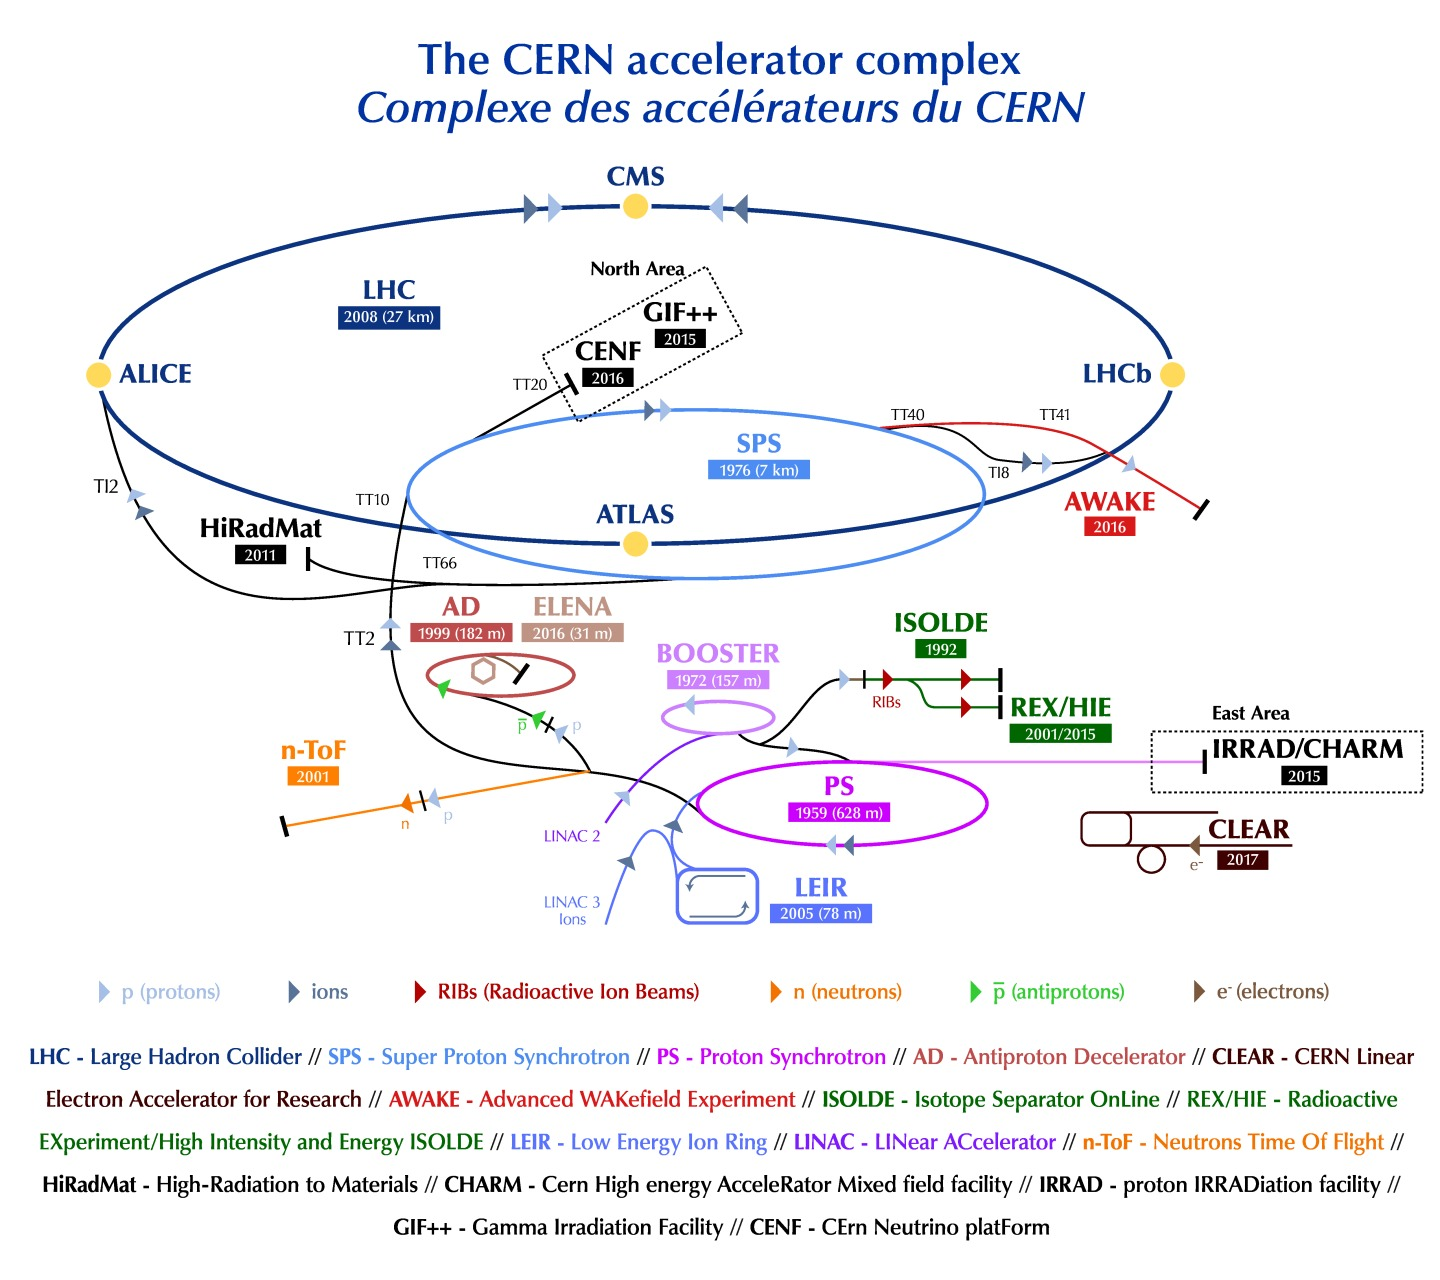
\includegraphics[width=\figwidth]{figures_LHC/CCC-v2018-print-v2.jpg}
\caption[Sketch of the LHC accelerator complex]{Sketch of the LHC accelerator complex showing the acceleration systems and the main storage ring with its experiments.~\cite{Mobs:2636343}}
\label{fig:accelerator_complex}
\end{figure}

\begin{figure}[htbp]
  \centering
  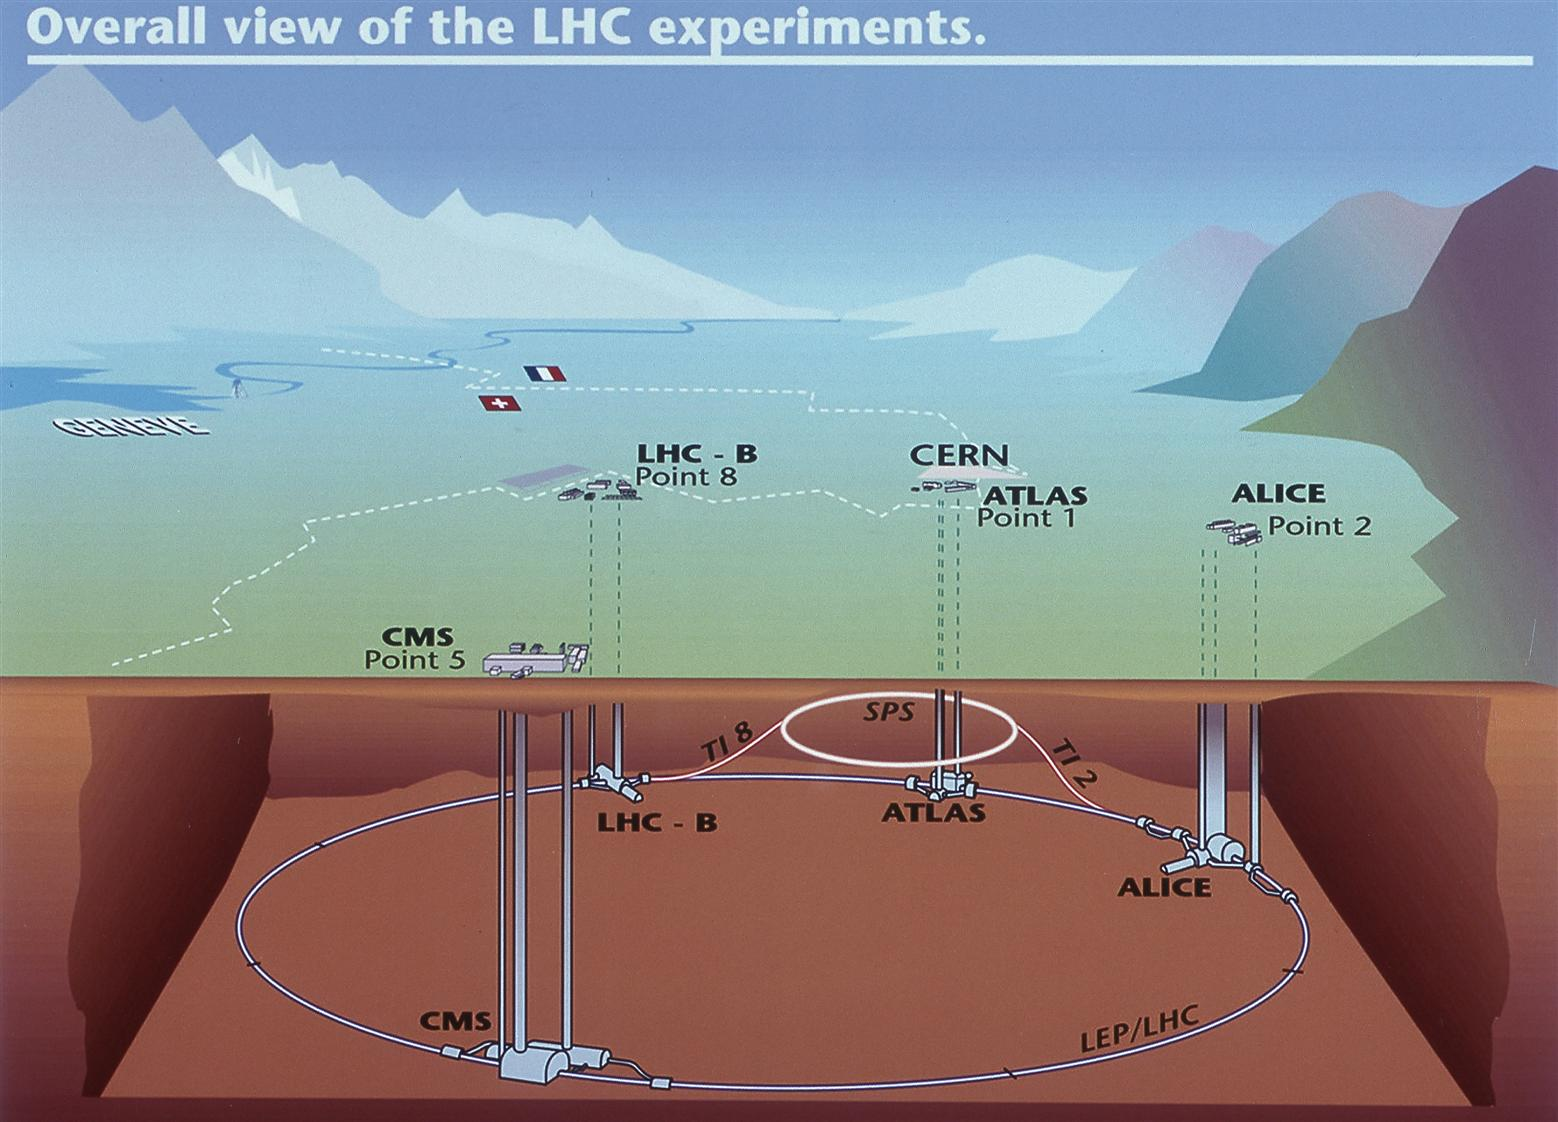
\includegraphics[scale=0.4]{figures_LHC/CERN-all-experiments.jpg}
  \caption[Sketch of the LHC ring.]{Sketch of the LHC ring, the position
    of the experiments and the surrounding countryside. The four big
    LHC experiments are indicated (ATLAS, CMS, LHC-B and ALICE) along with their injection lines (Point 1, 2, 4, 8).~\cite{Jean-Luc:841555}}
  \label{fig:LHC}
\end{figure}


\section{The ATLAS detector}

The ATLAS detector is a general purpose detector meaning it aims at covering a maximum number of final states, enabling reasearchers in may topics of particle physics to use its data.

ATLAS, \enquote{A Toroidal LHC Apparatus} has the distinguishing structure of a general purpose detector, its innermost part formed by tracking detectors directly surrounding the interaction point, followed by calorimeters, and a final layer for muon tracking. All the components are visualized in figure~\ref{fig:atlas} including two humans to give an impression of the detector's size.

The innermost tracking detectors are summarized under the name Inner Detector (ID) and consist of two silicon detectors namely the Pixel Detector and the Semi Conductor Tracker as well as a straw detector named Transition Radiation Tracker. The Inner Detector allows for precise measurement of not only charged particles' position, and thus vertex information, but also for their charge and momentum.

The calorimeter system is divided into two components, being the electromagnetic calorimeter and the hadronic calorimeter, allow to measure the energy of particles by stopping them in the detector material.

The Muon Spectrometer is the last tracking detector which identifies particles crossing it as muons, as all other charged particles are usually stopped in the calorimeter system.

In the following the concept of each detector component is briefly introduced~\cite{wermes} to then summarize how particles can be detected and distinguished. The reconstruction of objects from the detector response is explained and an event selection for \tW candidates introduced.



\begin{figure}[htbp]
  \centering
  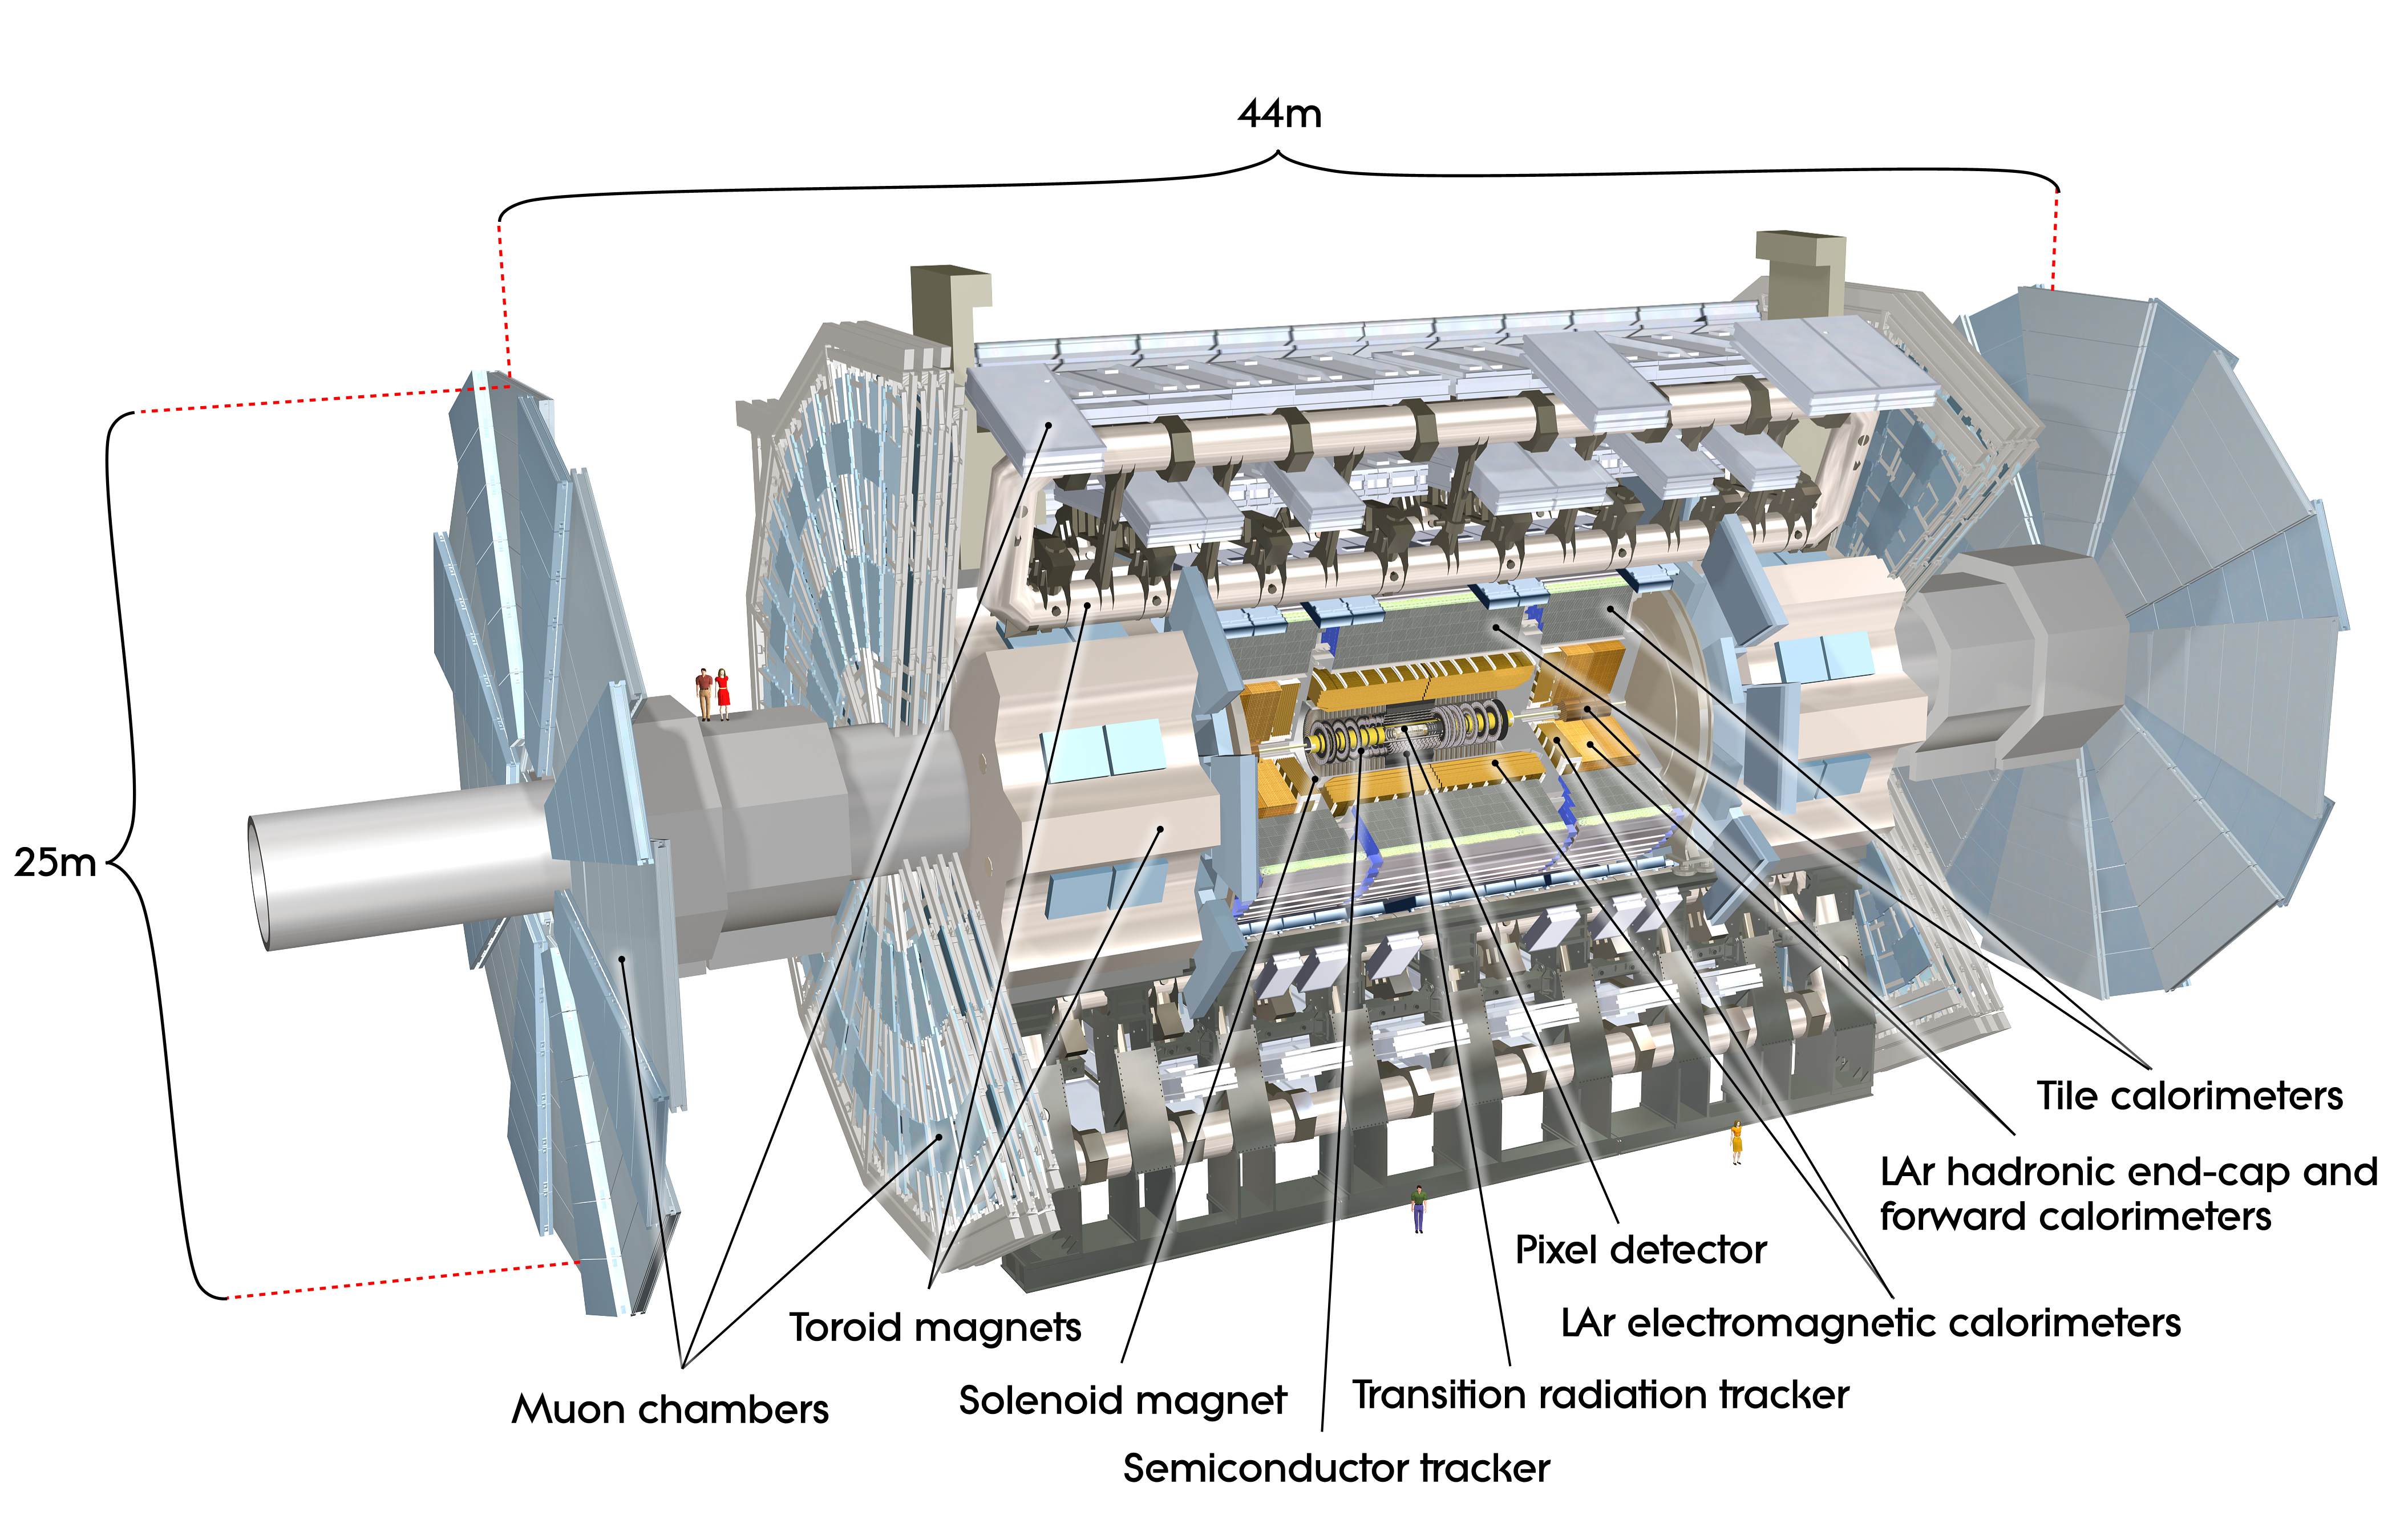
\includegraphics[scale=0.15]{figures_LHC/atlas-detector}
  \caption[Sketch of the ATLAS detector]{Sketch of the ATLAS detector and all its components including two average humans for scale.~\cite{Pequenao:1095924}}
  \label{fig:atlas}
\end{figure}


\subsection{Tracking detectors}

Tracking detectors are used to measure a charged particle's trajectory, momentum and charge value, of which two types are used in the ID of the ATLAS detector. The Pixel detector and the Semi Conductor Tracker (SCT) are silicon detectors and the Transition Radiation Tracker (TRT) is a straw-based tracking detector. For all detectors it holds true that they are surrounded by a magnetic field and cover a pseudorapidity range of $|\eta| < 2.5$. The magnetic field results in curved trajectories enabling an estimate of momentum and charge.\cite{leo}

Pixel detectors are based on ionisation of charged particles in the semiconductor material. The induced charge is picked up by the detector's pixels providing a position information. To provide a 3-dimensional trajectory the pixel-chips are ordered in 4 layers around the beam pipe where the layer closest to the point of interaction, called Insertable B-Layer (IBL), was added in 2015. It is located only \SI{3.3}{\centi \metre} from the beam pipe and allows to detect vertices very close to the interaction point mainly originating from \Pbottom-quarks giving the layer its name.~\cite{pixel_run2}

The SCT as a silicon microstrip detector is the second silicon-based tracker immediately following on the pixel detector. It consists of modules of four silicon strip sensors organised in four barrel layers and eighteen planar endcap disks.

The TRT is structured in straw tubes each tube being an individual drift chamber with a strong potential difference due to negatively charged walls. The tubes are filled with a gas mixture (\ce{Xe} or \ce{Ar}) causing transversing charged particles to ionize and then by accelerated to the walls. A cascade is initiated and a measurable signal in the potential difference is measured. 
Between the tubes material is inserted resulting in transition radiation. This radiation has a cross section way higher for electrons than for other particles over a wide range of energy thus adding particle information to the track information provided by the TRT.

A particle being detected in a layer of the ID is called a hit. The record of hits gives an estimate on the particle's trajectory and can thereby also provide information on the vertex the particle originates from. This vertex information is worth mentioning as for a an experiment with an event count as large as the ATLAS experiment's events interfere and information from so called pileup events can affect the event's information. As pileup originates from different events it can be separated from the event of interest by separating the vertices.

\subsection{The ATLAS calorimeter system}

The ATLAS calorimeter system is divided into three main parts. The electromagnetic (EM) calorimeter, comprising a barrel and two end-caps, and the hadron calorimeter, built by a tile calorimeter, consisting of a a barrel and two so called "extended barrels", and the hadron end-caps. The third part is the forward calorimeter which additionally focuses on electromagnetic interaction. The tile calorimeter is scintillator-based apart from that the main part of the calorimeter system is based on liquid argon. The components cover a pseudorapidity range of $|\eta| < 4.9$

Calorimeters determine a traversing particle's energy by exploiting the formation of particle showers.~\cite{wermes} Due to inelastic collisions in the detector's material, the energy of the original particle is distributed on a cascade of secondary particles finally stopped by ionization. The resulting charge or photons can be measured as an estimate of the initial energy.

Electromagnetic calorimeters exploit the energy loss of electromagnetically interacting particles in matter. Mainly photons and electrons loose their energy based on pair production and Bremsstrahlung respectively. The energy loss initializes a cascade of particle decays called an electromagnetic shower. The decay stops when the shower particles do not hold sufficient energy for a decay anymore. The energy of the final state shower particles is picked up by the detector representing the initial particle's energy.
The ATLAS ECAL is a sampling calorimeter, built of two alternating layers of absorber and detection material. In the absorber the showers are induced to subsequently be detected in the detection layers.


As the ECAL uses electromagnetic showers the hadronic calorimeter depends on hadronic shower evolution. Hadronic showers are initialized due to ionisation or strong interaction with the material's nuclei. If the resulting particles still interact with the material a shower evolves.
The hadronic tile calorimeter is made of alternating layers of steel absorbents and scintillators covering a pseudorapidity range of $|\eta| < 1.6$.
The hadronic endcap calorimter (HEC) is liquid argon-based and covers $1.4 < |\eta| < 3.1$
Due to the larger size of hadronic showers the HCAL occupies more detector space than the ECAL.


\subsection{The Muon spectrometer}

The second tracking detector of ATLAS is the muon spectrometer which is the outermost part of the detector. The task of the spectrometer is to detect charged particles traversing the calorimeter without being stopped or deploying their complete energy, and to do both collect trigger information and information on trajectory and momentum. Due to these two tasks the spectrometer is bifid with the first part being the trigger chamber covering a range of $|\eta|<2.4$, followed by the high-precision chamber with a range of $|\eta|<2.7$. The main detector's support feet cause a further gap at about $\phi = \ang{300}$ and $\phi = \ang{270}$.

Normally the only charged particles left to be detected in the muon spectrometer are muons giving the component its name and allowing to provide good trigger information for researches interested in muons in the final event topology.




\subsection{The ATLAS coordinate system}

The ATLAS coordinate system is a right-handed and right-angled coordinate system with the $z$-axis pointing along the LHC's beam pipe. The corresponding transverse plane is defined by the $x$-axis pointing towards the ring's centre while the $y$-axis points upwards. The origin of the system is defined by the nominal point of interaction. The polar angle $\theta$ is the angle between the $z$-axis and the $x$-$y$-plane and the azimuthal angle $\phi$ is the angle between the $x$- and the $y$-axis.

Alternatively, as in this work, an event's topology is described by the azimuthal angle $\phi$, the pseudo-rapidity $\eta$, and the transverse momentum \pT. The pseudo-rapidity replaces the polar angle and is defined as

\begin{equation}
\eta = \frac{1}{2} ln\left[ tan\left(\frac{\theta}{2}\right)\right].
\end{equation}

The transverse momentum is defined by

\begin{equation}
\pT = \sqrt{p_x^2 + p_y^2}
\end{equation}
where $p_x$ and $p_y$ are the momenta along the corresponding axes. 

The angular variables are defined within

\begin{equation}
\eta \in [-\infty,\infty],\,
\phi \in [-\pi,\pi].
\end{equation}

This cylindrical system makes use of the shape of the ATLAS detector and the momentum conversation of the transverse plane due to it being perpendicular to all initial beam momenta.

\subsection{Particle Detection in the ATLAS detector}

This section focuses on the detection and distinction of different particle types in the ATLAS detector. The capability and combined information of the detector components is introduced giving an explanation of the general working principle and also of the characteristics defining the events in this work. Figure \ref{fig:atlas_sketch} gives an overview of typical particle interactions and detections.

In order to reconstruct the particles in an event low level information is gathered using the direct detector output and then associated to the higher level particle information.

The information from the ID is called a track and contains not only the trajectory but also tells how consistently a track holds hits in every layer. A track offers momentum and charge information and can be associated with a vertex and a possible energy deposition in a calorimeter. 
The vertex reconstruction arising from the track information allows to define a primary vertex defined by the highest sum of squared transverse momenta while additional vertices are identified as pileup vertices.
Secondary vertices originating from tracks connected to the original vertex can be collected to identify short-lived particles.

The calorimeter data is summarised in clusters. Clusters are neighboring calorimeter cells with energy depositions significantly higher than the expected noise. A cluster is formed around a high energy deposition and can be associated to hadrons or jets or even to a corresponding track.

In the following the higher order objects reconstructed from this basic information are introduced to then explain the decisions made in the event selection for the \tW channel.

\begin{description}
\item[Electrons] 
are constructed from energy deposits in the EM associated with ID tracks.
To improve the decision rule, a likelihood object quantity is constructed from the shape and the ratio of the calorimeter to tracker response, and a set of further variables suitable for a better discriminant. There are three settings for the likelihood object namely tight medium and loose depending on how restrictive the analysis is.
Lastly an isolation quantity is defined based on cones around the track and the EM deposit to further decimate background and fake electrons.~\cite{ATLAS-CONF-2016-024}
\item[Jets] are cones of particles originating from the common hadronisation of a quark or gluon. In the detector they are reconstructed using 3-dimensional topological clusters of calorimeter energy.~\cite{Aad:2016upy} In addition to this there is further information that can be associated to jets, {i.e.}, an ID track or a vertex using a jet-vertex-tagger to minimize the impact of pile-up events and to associate to secondary vertices. For reconstruction the \antikt algorithm was used.~\cite{Cacciari:2008gp}
\item[Muon] reconstruction uses MS hits matched with ID tracks. The choice can be further specified by applying an identification cut based on MS/ID agreement and integrity of MS hit response. As for electrons isolation can be required.~\cite{Aad:2016jkr}
\item[\Pbottom-jets] are jets originating from the decay of a \Pbottom-quark and therefor a strong discriminant for events containing a \Ptop decay. The process of identifying a \Pbottom-jet is called \Pbottom-tagging and uses a multivariate discriminant. The topology of \Pbottom-jets is distinguishable from other jets due to for example clear secondary vertices, vertex alignment of a primary, a secondary \Pbottom-vertex and a tertiary \Pcharm-vertex, the decay length, and the characteristic energy scale.~\cite{Aad:2110203, ATL-PHYS-PUB-2016-012}
\item[Missing transverse momentum]
arises from momentum imbalance in the transverse plane. Momentum in the transverse plane should be preserved due to it being perpendicular to the beam axis and imbalance is an indicator for neutrinos escaping the detector. It is calculated using two contributions, one being signals from fully reconstructed and calibrated particles and the other one is information from reconstructed charged particle tracks. ~\cite{Aaboud:2018tkc}  
\end{description}

In addition to this the ATLAS trigger system has to be mentioned. Although potentially deserving a chapter of its own for this work it is sufficient to just state  and briefly explain trigger information.

Triggers are used to filter events before the actual event selection is taken into account. Given the incredible luminosity of the LHC such a preselection is important to minimize the data actually processed by the more complicated analysis algorithms and selection schemes.
The ATLAS trigger system consists of three triggers, namely the Level 1 (L1), Level 2 (L2), and the Event Filter (EF) where L2 and EF are generally referred to as the High-Level Trigger (HLT).

The L1 is is completely hardware-based and its decision making process is motly based on information from the calorimeter and the muon trigger chambers. The decision step relies on high-\pT objects and their multiplicity in an event while also considering missing transverse momentum and the beam condition to provide a first and very broad event selection.

The HLT is based on software and takes the L1 events as input. L2 defines so called regions of interest (ROI) as those regions in the angular plane where the trigger objects for L1 were detected and applies further trgger cuts to these objetcs.
The EF fully analyzes the event based on the complete information available.

This trigger information can be used for event selection making sure that certain final state objects are dominant in the topology and also to just apply a first, broad selection.



\begin{figure}[htbp]
  \centering
  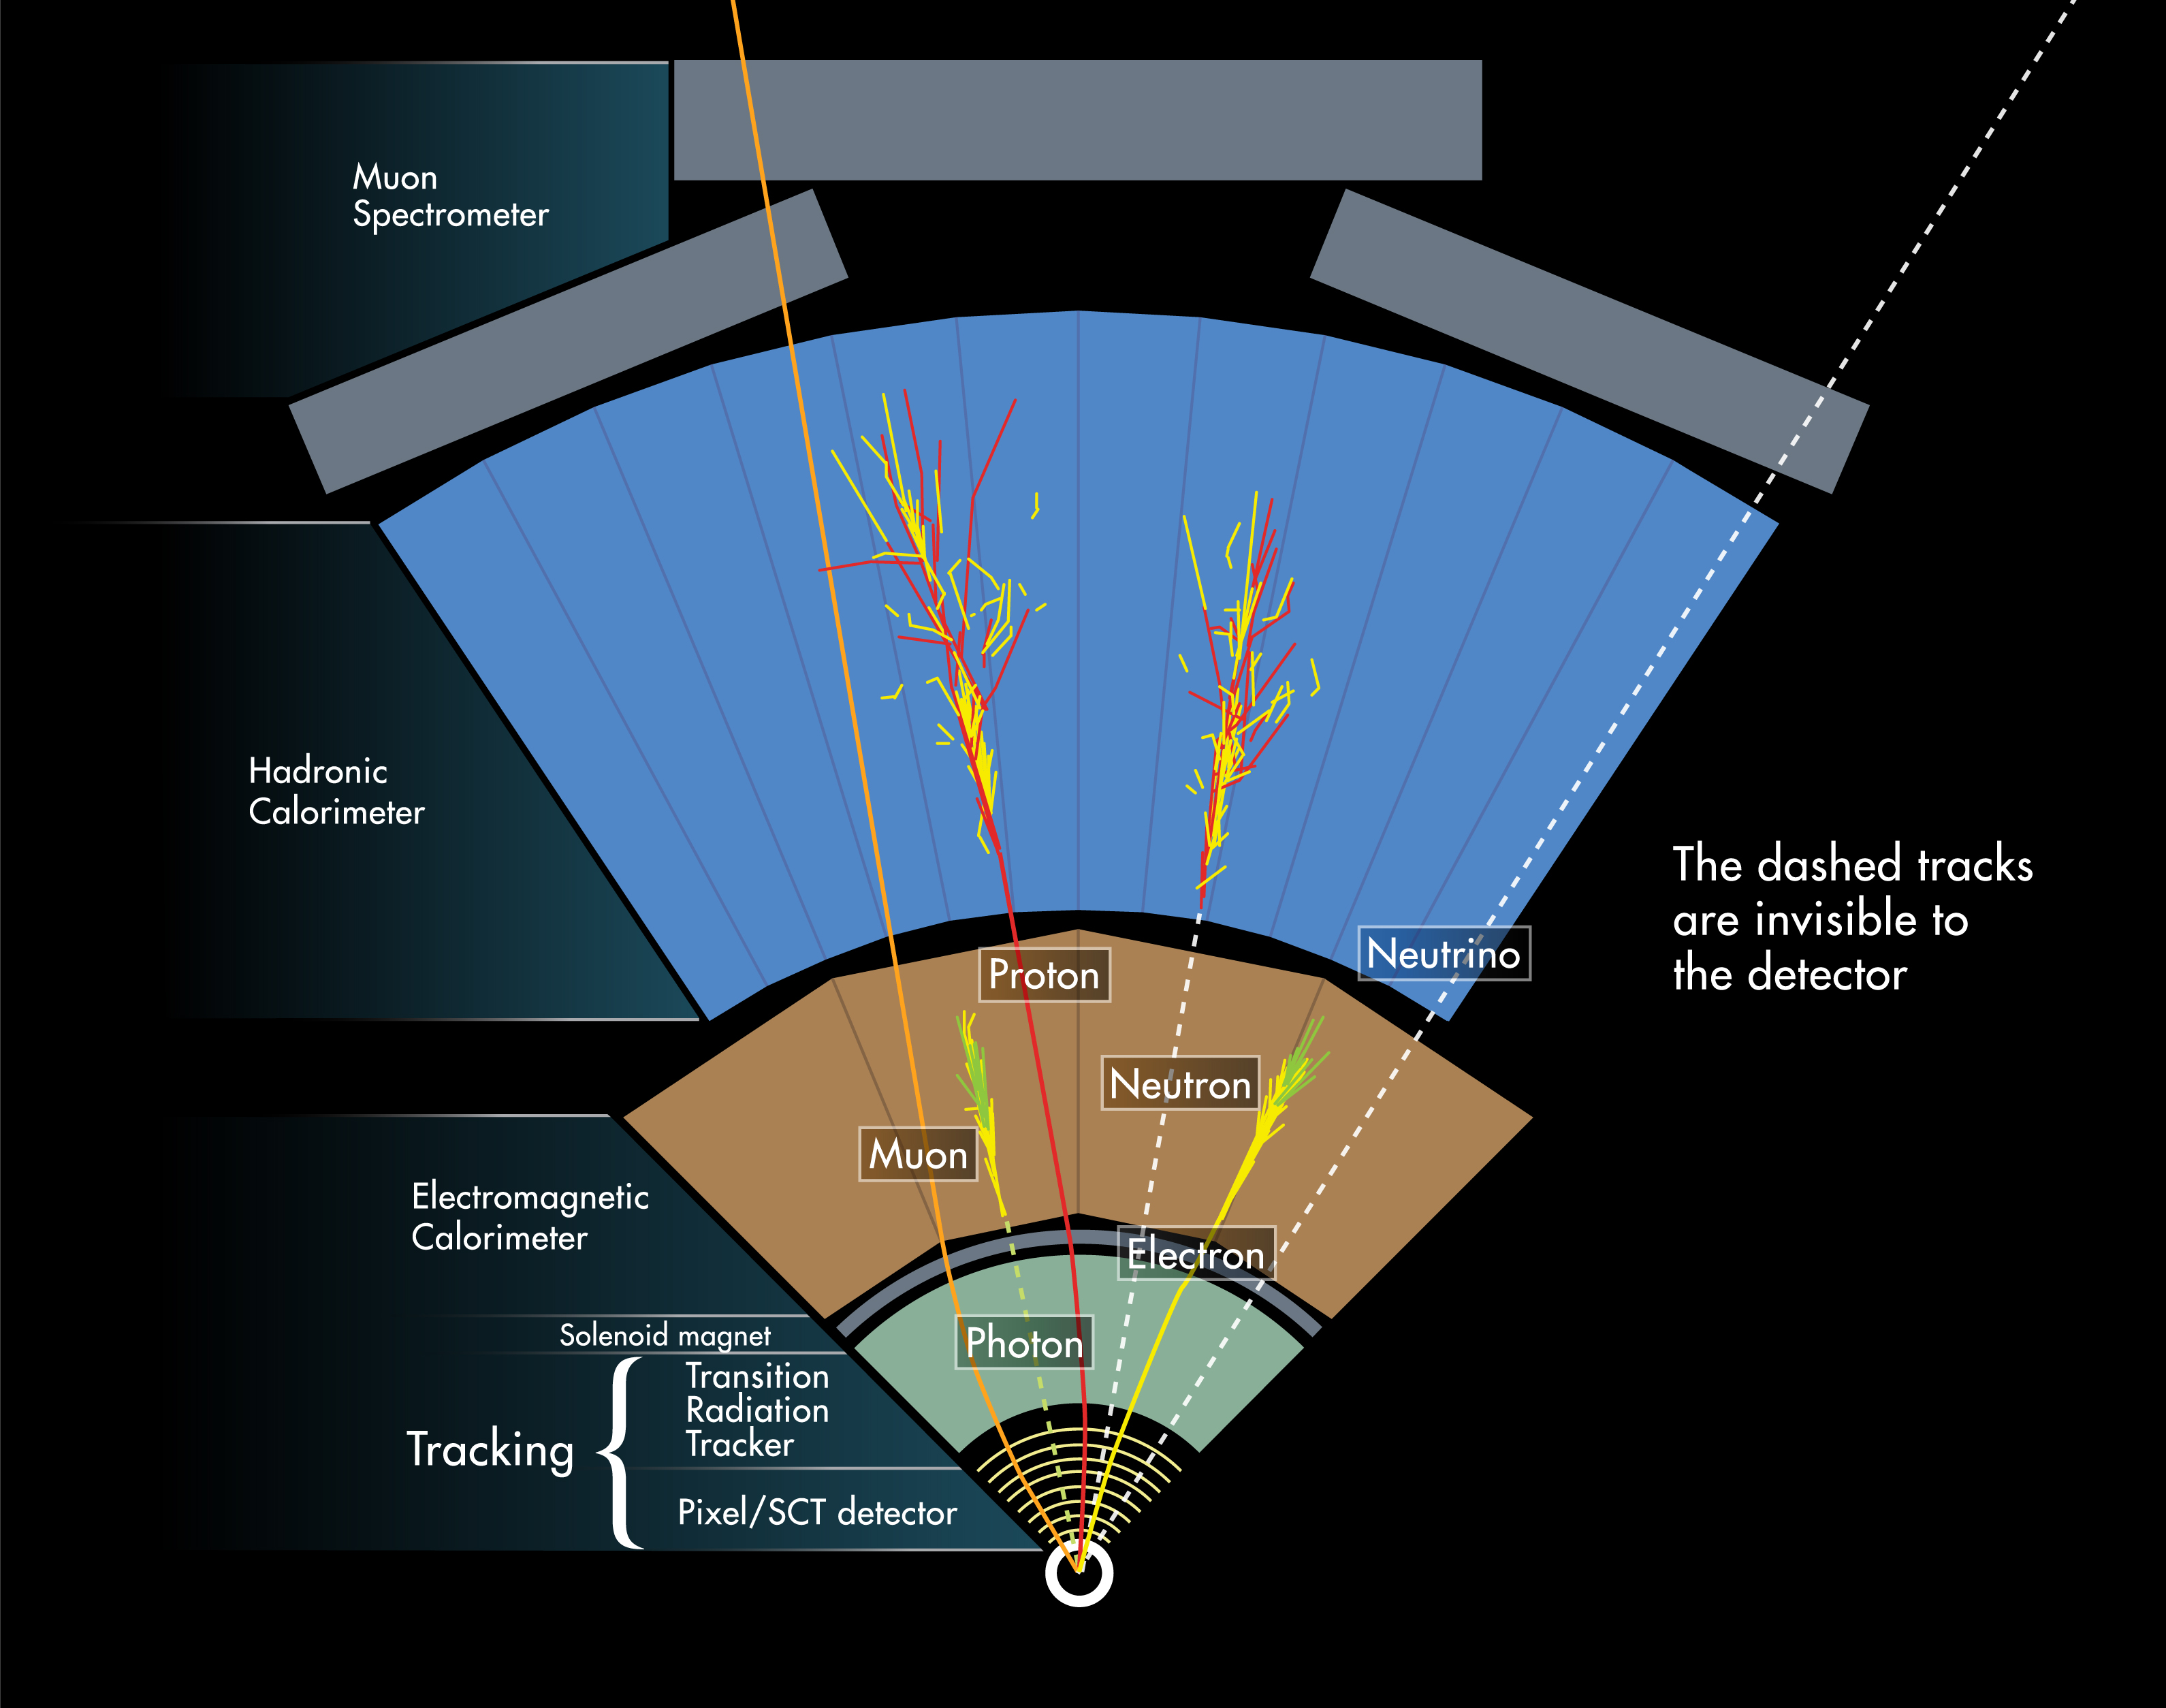
\includegraphics[scale=0.6]{figures_LHC/atlas-abstract}
  \caption[Scheme of the ATLAS-detector's detection procedure]{Scheme of the ATLAS-detector showing examples of typical particle detections. \cite{Pequenao:1095924}}
  \label{fig:atlas_sketch}
\end{figure}


%A Monte Carlo simulation is a statistical simulation of a possibly deterministic system. 

%detector simulation runs on top of Monte Carlo simulation

%Simulations are based on cross sections which can be calculated and measured in units of \textsc{barn} where \SI{1}{\barn} = \SI{1e-28}{\square \metre}

%Simulations heavily rely on quantities than can both be calculated and measured in an experiment thus allowing for predictions and also for  controlling the theoretical values.
%In high energy particle physics there are mainly two such quantities cross section and branching ratio0

%In collisions not only the valence quarks but also the sea quarks are relevant which can be explained by the valence quarks radiating gluons and quark antiquark pairs with no net flavour change.also explains the mass

\section{tW event selection}

The process separation of interest for this work is \tW \ttbar. Other backgrounds for the \tW channel are reduced by applying an event selection:


\begin{itemize}
\item A single electron or muon trigger
\item Electrons: tightly identified, isolated, \ET > \SI{26}{\giga \electronvolt}
\item Muons: tight isolation, \pT > \SI{26}{\giga \electronvolt}
\item Opposite-charge lepton pair
\item Leading lepton \pT > \SI{27}{\giga \electronvolt}
\item Veto for a third lepton \pT > \SI{20}{\giga \electronvolt}
\item A lepton must match the trigger
\item At least one jet with: \pT > \SI{25}{\giga \electronvolt}, $|\eta|$ < \num{2.5}, tagged at \num{77} \% working point
\end{itemize}

After this preselection the events are categorized in regions based on the jet and \Pbottom-jet multiplicities. For this work the region with exactly two \Pbottom-tagged jets was used denoted as \texttt{2j2b}. This region has especially high impact from the NLO interference with a \Ptop\APtop final state.

\section{Monte Carlo simulation}

A Monte Carlo simulation is a computer based stochastic calculation of a process that in principle could be deterministic but the problem and the amount of statistics suggest a stochastic approach.

Monte Carlo for the ATLAS detector is the simulation of detector events to calibrate the performance and generate an estimator to compare model and measurement. As for for this work the classifying tools and event selection rules are tested and tuned based on simulations to achieve a better understanding of what efficiencies are to be expected in a data analysis. This provides the truth information to an event that is needed for supervised learning, see section \ref{chp:ml}, and cannot be provided by data.

A simulation has to be based on quantities that can not only be calculated from theoretical models but also measured during the experiment because an interplay between simulation and actual data is needed to adjust the simulation to the experimental circumstances. In collider physics predictions are mainly based on  the cross-section of an interaction stating how high the probability for certain interaction is. In addition to that the decay width of a particle is needed to describe how particles generated in an interaction behave in the detector system.

A proton-proton collision is modeled by describing the protons as a sea of partons, {i.e.}, the gluons and quarks their momentum is carried by, and then calculating the cross-sections for these partons to interact individually. The technique of seeing the collision as an interaction of two individual partons while decoupling these interactions from the parton interactions in the individual protons is called factorization.
For a parton carrying the fraction $x$ of the proton's momentum for a center-of-mass energy of $\hat{s}$  the cross-section $\sigma(p_1 p_2 \rightarrow X)$ to create a final state $X$ can be described as:


\noindent\begin{minipage}{.5\linewidth}
\begin{equation}
	x_i = \frac{p_{parton,i}}{p_{proton}} 
\end{equation}
\end{minipage}%
\begin{minipage}{.5\linewidth}
\begin{equation}
	\hat{s} = x_1 x_2 s
\end{equation}
\end{minipage}

\begin{align}
	\sigma ( p_1 p_2 \rightarrow X ) = \sum_{i,j = \Pquark, \APquark, \Pgluon} \int dx_i dx_j f_{i/p_1} ( x_i, \mu^2 ) f_{j/p_2} ( x_j, \mu^2 ) \cdot \hat{\sigma}_{ij} ( ij \rightarrow X; \hat{s}, \mu^2 )
\end{align}

There are two quantities in this equation not yet explained.
The first on is the parton density function (PDF) of the proton denoted as $f_{i/p_m} ( x_i, \mu^2 )$. This is a function describing the probability that a parton with momentum fraction $x_i$ in the proton $k$ takes part in the hard scattering. The PDF is independent of the collision and has to be gained from experiments rather than through calculations.

The second quantity $\mu$ is the so called factorization scale. It describes to which degree the interactions of the partons in the proton can be neglected. It is an arbitrary scale determining the precision of the simulation to some degree.

\subsection{ATLAS simulation}

The MC simulation for the ATLAS detector is generated in two steps.~\cite{atlasmontecarlo}

In the first step the actual collision is simulated defining the particles in the final state. The underlying algorithm is called Monte Carlo event generator.

Secondly the response of the detector to these particles is simulated by the detector simulation allowing objects to be reconstructed from the event like from actual data gaining a comparison on every level of reconstruction.

Furthermore a set of different options and generators can be chosen for the simulation. Examples would be how a parton shower is simulated or to which degree multi parton interaction is taken into account.

\subsection{Systematic uncertainties in Monte Carlo simulations}

Simulations as described earlier have to be based on certain assumptions about the input parameters especially in those cases where the theory does not offer a precise result. This results in systematic uncertainties arising from the simulations and it is not obvious how good the actual data is represented by the assumptions made.
In those cases different Monte Carlo samples are produced each representing a different assumption about the initial parameters showing first of all how the data should behave with these scaled paramters and allowing to test whether the systematic or the original sample fits better to the data. 
These samples of Monte Carlo will just be referred to as systematics in this work.

Usually the simulations use the leading order cross-section.
When next-to-leading order diagrams become relevant the simulation has to be adapted resulting in different samples for different orders.
This work focuses on the \tW and \ttbar events interfering at NLO as described in \ref{chp:tw}
The total NLO amplitude is the sum of the of singly resonant diagrams and all doubly resonant diagrams:

\begin{align}
\Aamp = \Atw + \Att
\end{align}

Calculating the cross-section requires the square of this amplitude:

\begin{align}
|\Aamp|^2 &= |\Atw|^2 + 2 \mathcal{R} \{ \Atw \Att^{\ast} \} + |\Att|^2 \\
&\equiv \Samp + \Iamp + \Damp
\end{align}

As a nominal sample in this work the Diagram Removal approach, denoted as DR, is used. It fully removes the \Att amplitude and thus both the pure \ttbar contribution as well as the interference term vanish.

\begin{align}
| \ADR |^2 = \Samp
\end{align}

Alternatively the Diagram Subtraction or DS can be used which is in this work represented by the systematics sample. It introduces a gauge invariant term that cancels the \ttbar contribution and in a simplified way can be written as

\begin{align}
| \ADS |^2 &= \Samp + \Iamp + \Damp - \widetilde{\Damp}\\
&\approx \Samp + \Iamp.
\end{align}

The nominal samples were produced using a full ATLAS detector simulation implemented in \GEANTfour and the systamtic samples were mostly simulated using \ATLFASTtwo.~\cite{geant, atlfast}

The events were generated by \POWHEG\PYTHIA8.~\cite{pythia}

%---------------------------------------------------------------------


\missingfigure{DR/DS}
\chapter{The tW Channel}
\label{chp:tw}

For the first part of this chapter the decay of the top-quark is discussed. Then the production channels of the top-quark are diagrammed. Finally the production channel of interest and its final state are explained in the context of its background at the Large Hadron Collider (LHC). For more information about the LHC see chapter~\ref{lhc_atlas}.
The diagrams shown in this chapter were created using the code available at~\cite{feyn_repo}.

\section{Top-quark decay}


\section{Top-quark production}

Most commonly top-quarks are created via the strong force in a top- anti-top-quark final state. Both gluon-gluon fusion and \Pquark\APquark-annihilation are possible production processes are possible. Figure~\ref{fig:ttpairLO} shows the processes at leading order (LO). Leading order means that no corrections for additional gluon emission and virtual corrections were taken into account.

\begin{figure}[htbp]
  \begin{subfigure}[b]{0.3\textwidth}
  	\centering
    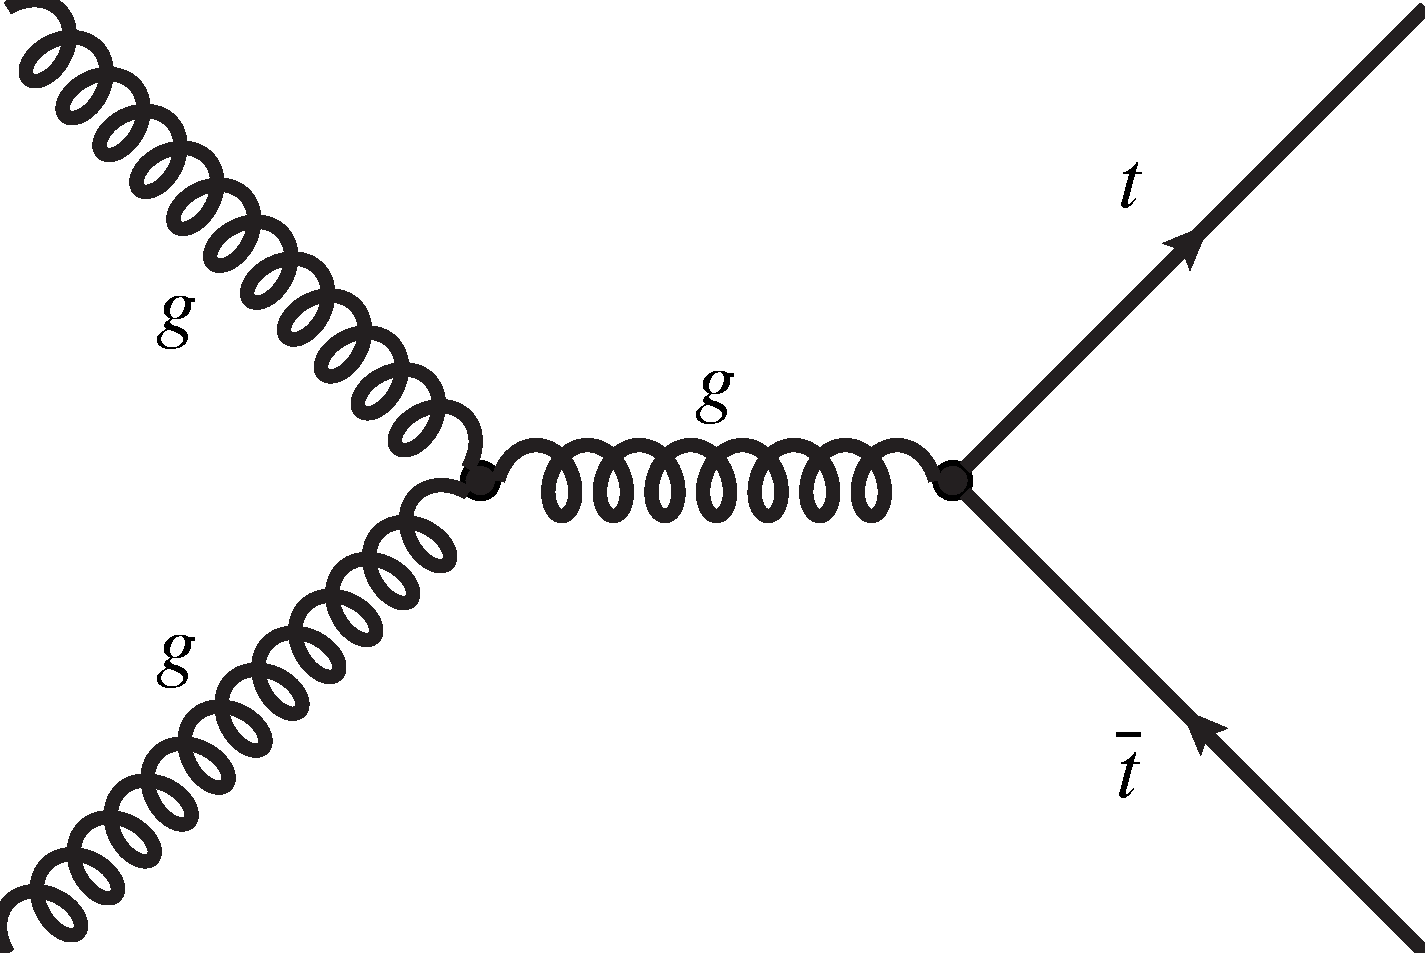
\includegraphics[height=3.5cm]{ttbar_ttbar_1-BW}
%    \caption{Picture 1}
%    \label{fig:1}
  \end{subfigure}
  \quad
  \begin{subfigure}[b]{0.3\textwidth}
  	\centering
    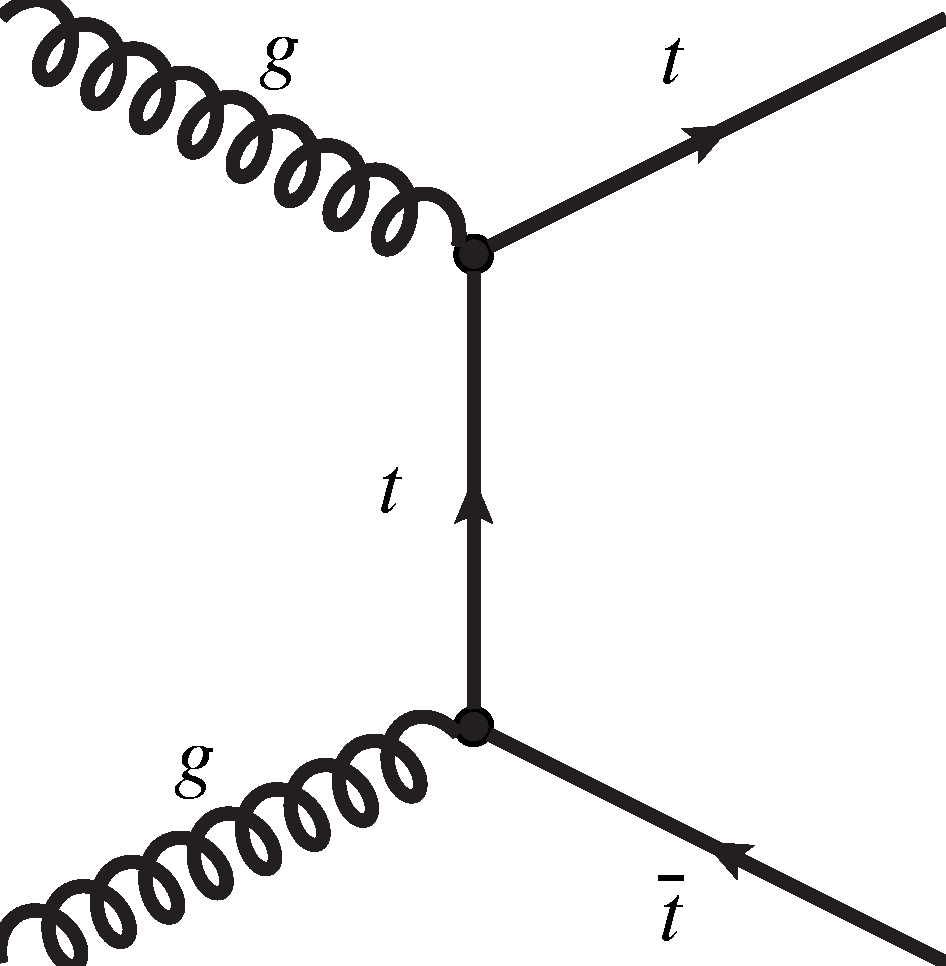
\includegraphics[height=3.5cm]{ttbar_ttbar_2-BW}
%    \caption{Picture 2}
%    \label{fig:2}
  \end{subfigure}
  \quad
  \begin{subfigure}[b]{0.3\textwidth}
  	\centering
    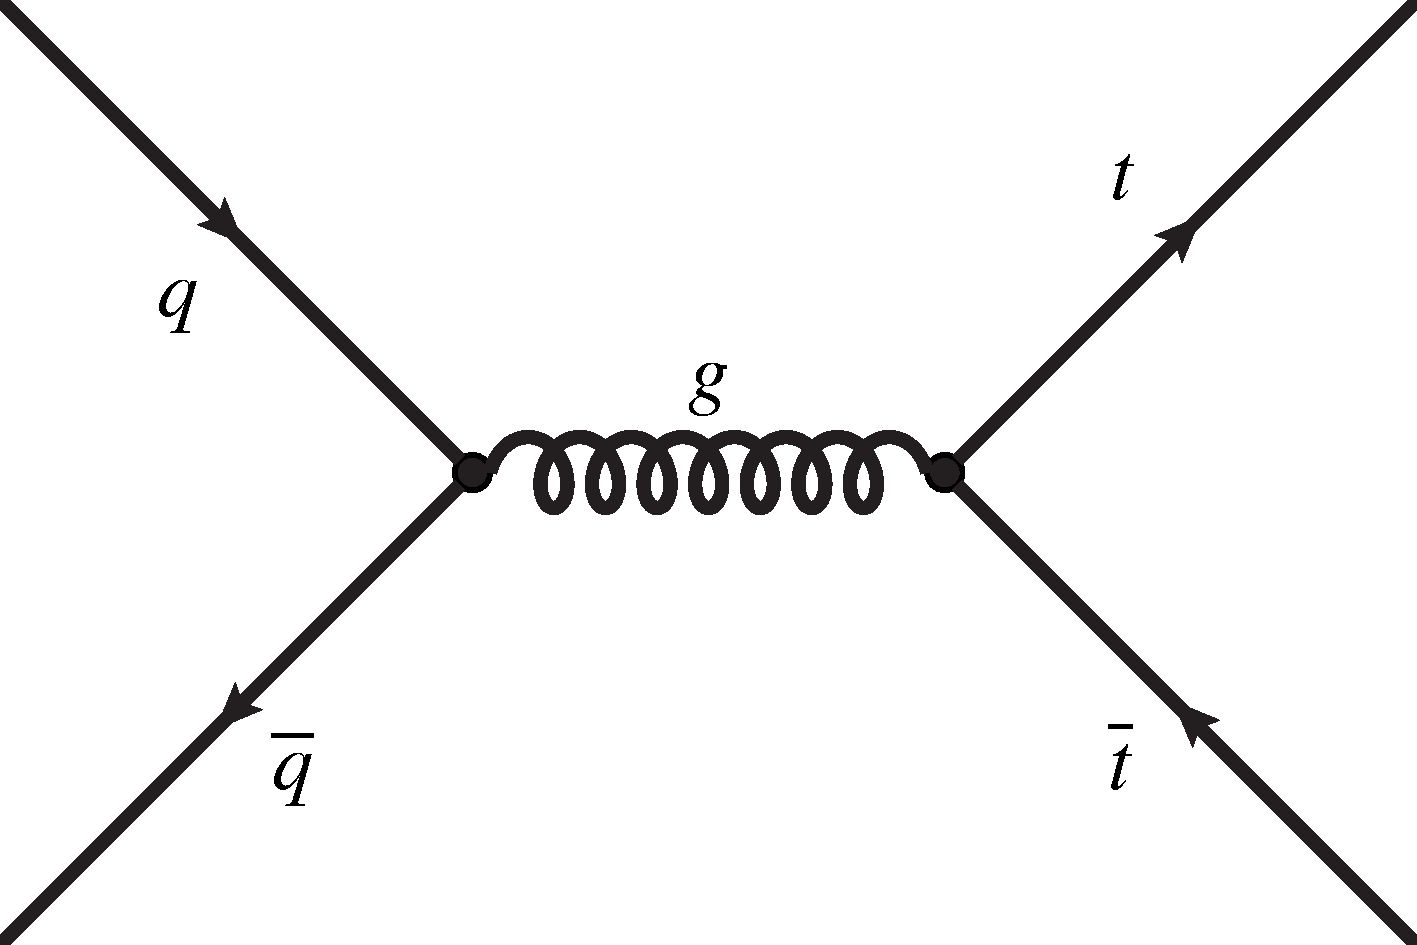
\includegraphics[height=3.5cm]{ttbar_ttbar_3-BW}
%    \caption{Picture 2}
%    \label{fig:2}
  \end{subfigure} 
  \caption{\ttbar pair production feynman diagrams at LO.}
  \label{fig:ttpairLO}
\end{figure}

Additionally, top-quarks can be produced as single top-quarks via the electroweak interaction. The dominant process is the production through the interaction of a bottom-quark and a \PW-boson shown in figure~\ref{fig:singletop:virtualWt}. Also possible but the least common is the s-channel involving a virtual \PW-boson displayed in figure~\ref{fig:singletop:virtualWs}. Finally the channel of interest for this work is the \tW-channel diagrammed in figure~\ref{fig:singletop:tW}.

Figure~\ref{fig:tw-decay} shows the final state of the \tW decay with both \PW-bosons decaying leptonically at LO. Therefore the channel is named dilepton channel.
At Next-To-Leading Order (NLO) a gluon splitting can result into a further bottom-quark in the final state. Figure~\ref{fig:nlo} shows the \ttbar final state in comparison to the NLO final state of the \tW-channel. In the final state these channels these channels are not distinguishable, {i.e.}, they interfere. These diagrams will be referred to as doubly resonant, in contrast to the singly resonant diagrams such as diagrammed in figure~\ref{fig:ttpairLO}.
Given that the \ttbar-cross-section is \num{10} orders larger than the \tW-cross-section this gives rise to a NLO correction exceeding the actual LO cross-section. This results in the \tW-channel not being well-defined at NLO.
To allow treating \tW as a separate process a workaround has to be used. There are two possible schemes for handling the interference in the calculation of the cross-section:

\begin{description}
\item[Diagram Removal (DR)] removes all diagrams containing a second top-quark propagator that can be on-shell. It is used for the production of the nominal sample in this work.
\item[Diagram Subtration (DS)] only the \ttbar contribution is cancelled when the top-quark is on-shell. This scheme is used for the systematics sample.
\end{description}

For more information on the schemes and their motivation see section~\ref{sec:systmc},

\begin{figure}[htbp]
  \begin{subfigure}[b]{0.3\textwidth}
  	\centering
    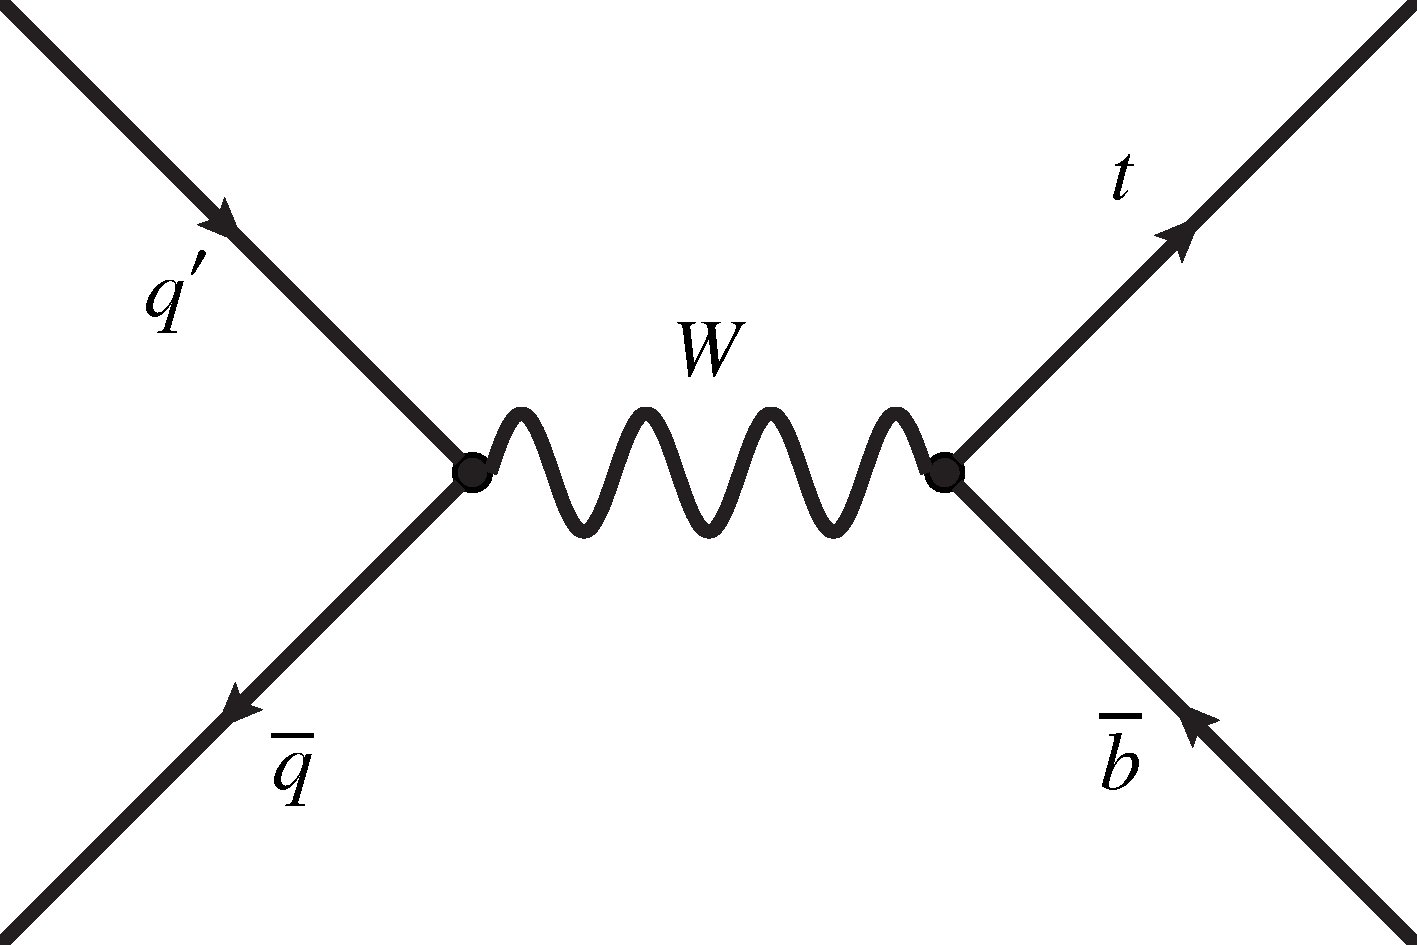
\includegraphics[height=3.5cm]{s-channel}
    \caption{}
    \label{fig:singletop:virtualWt}
  \end{subfigure}
  \quad
  \begin{subfigure}[b]{0.3\textwidth}
  	\centering
    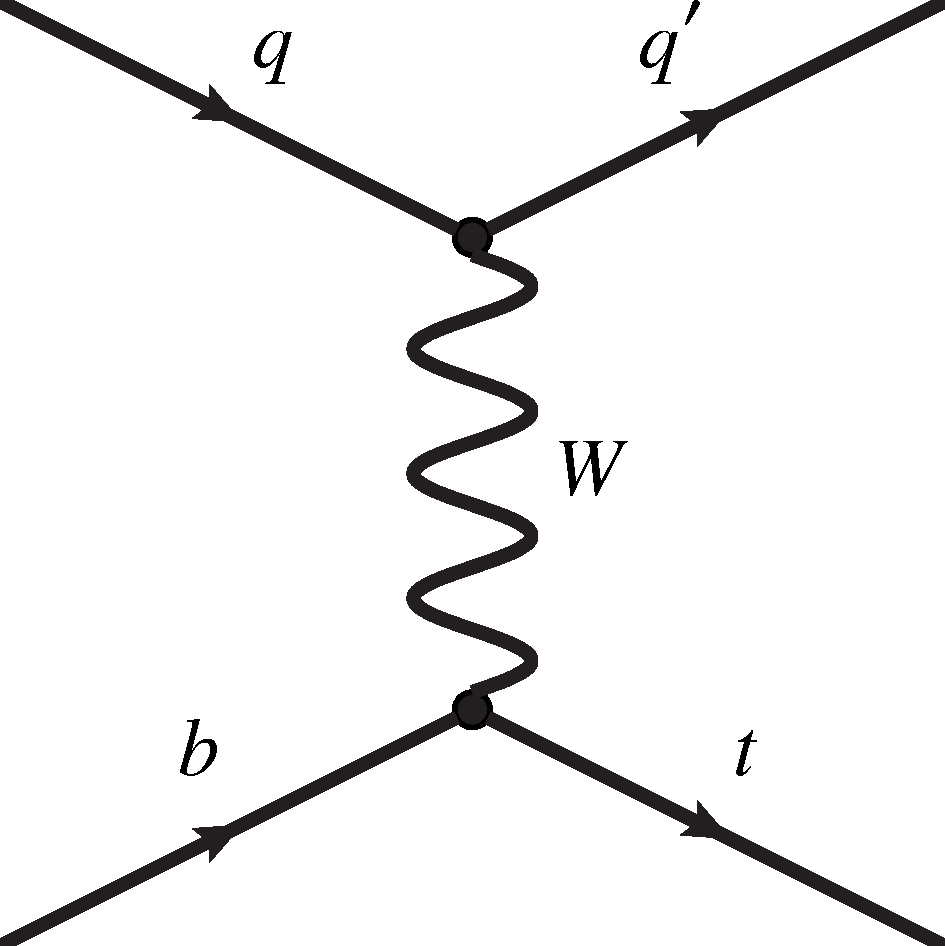
\includegraphics[height=3.5cm]{t-channel}
    \caption{}
    \label{fig:singletop:virtualWs}
  \end{subfigure}
  \quad
  \begin{subfigure}[b]{0.3\textwidth}
  	\centering
    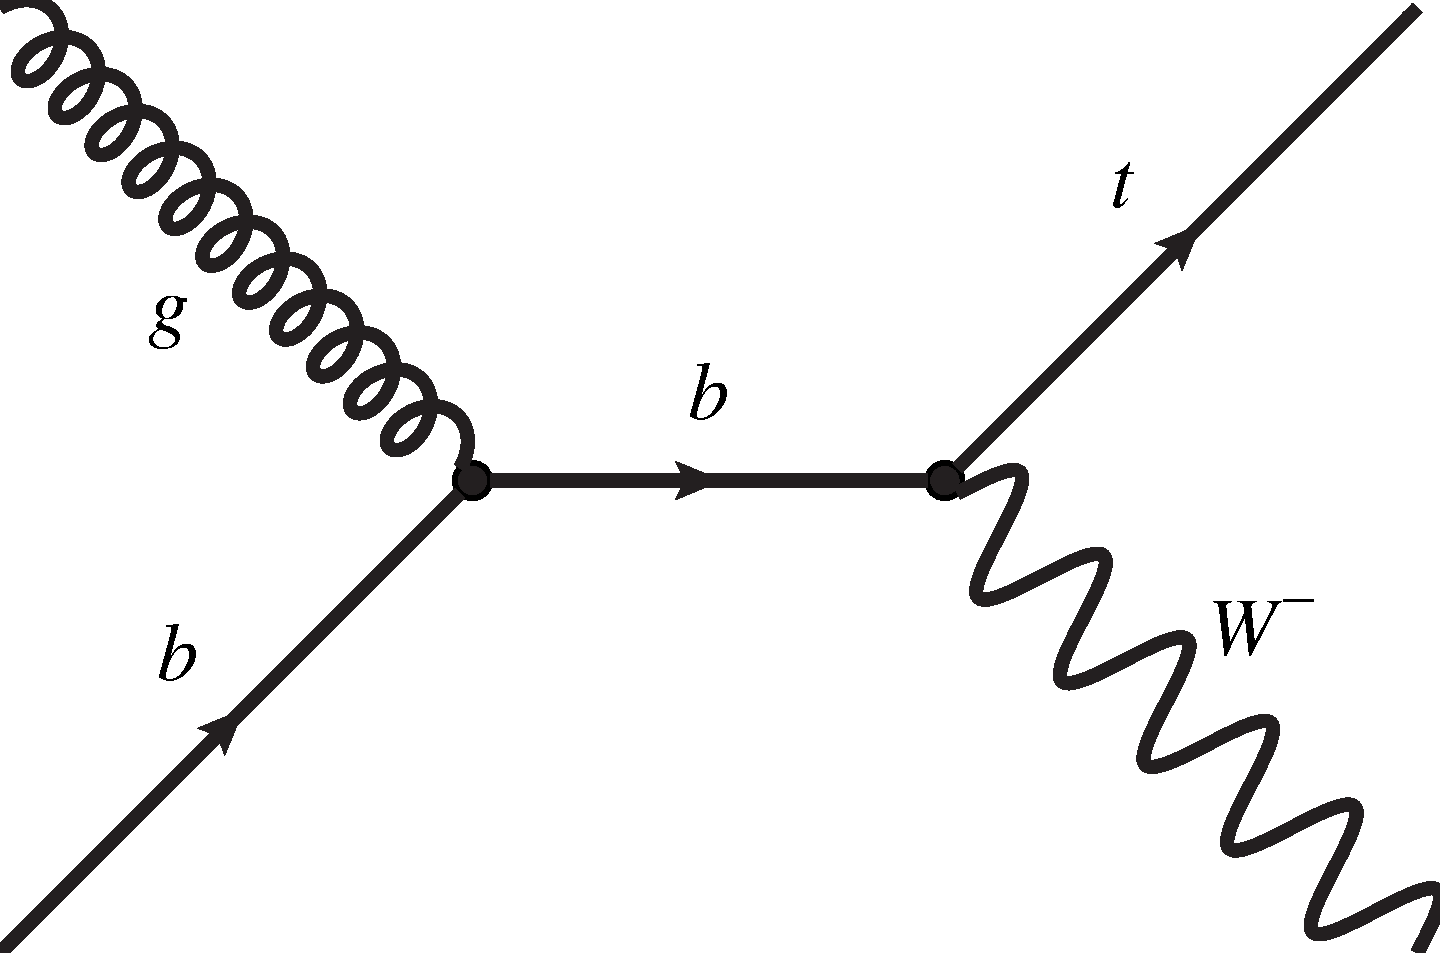
\includegraphics[height=3.5cm]{tW_channel}
    \caption{Picture 2}
	\label{fig:singletop:tW}
  \end{subfigure} 
  \caption{Single-top-production diagrams: s-channel~\subref{fig:singletop:virtualWs}, t-channel~\subref{fig:singletop:virtualWt}, \tW-channel~\subref{fig:singletop:tW}}
  \label{fig:singletop}
\end{figure}


\begin{figure}[htbp]
	\centering
	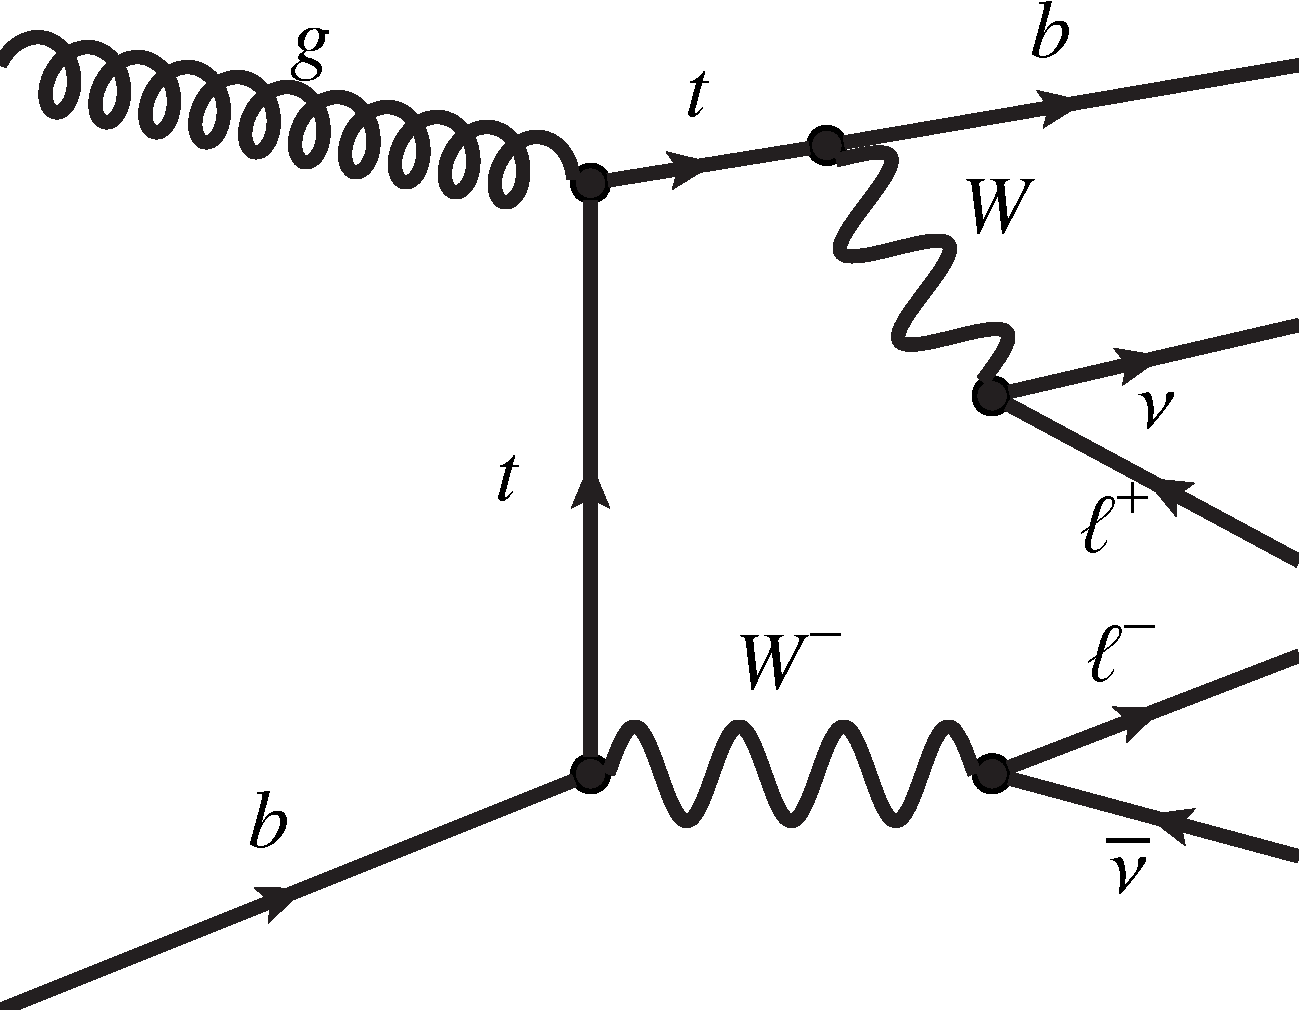
\includegraphics[width=0.8\textwidth]{tW-decay}
	\caption{text}
	\label{fig:tw-decay}
\end{figure}

\begin{figure}[htbp]
    \centering
    \begin{subfigure}[b]{0.44\textwidth}
        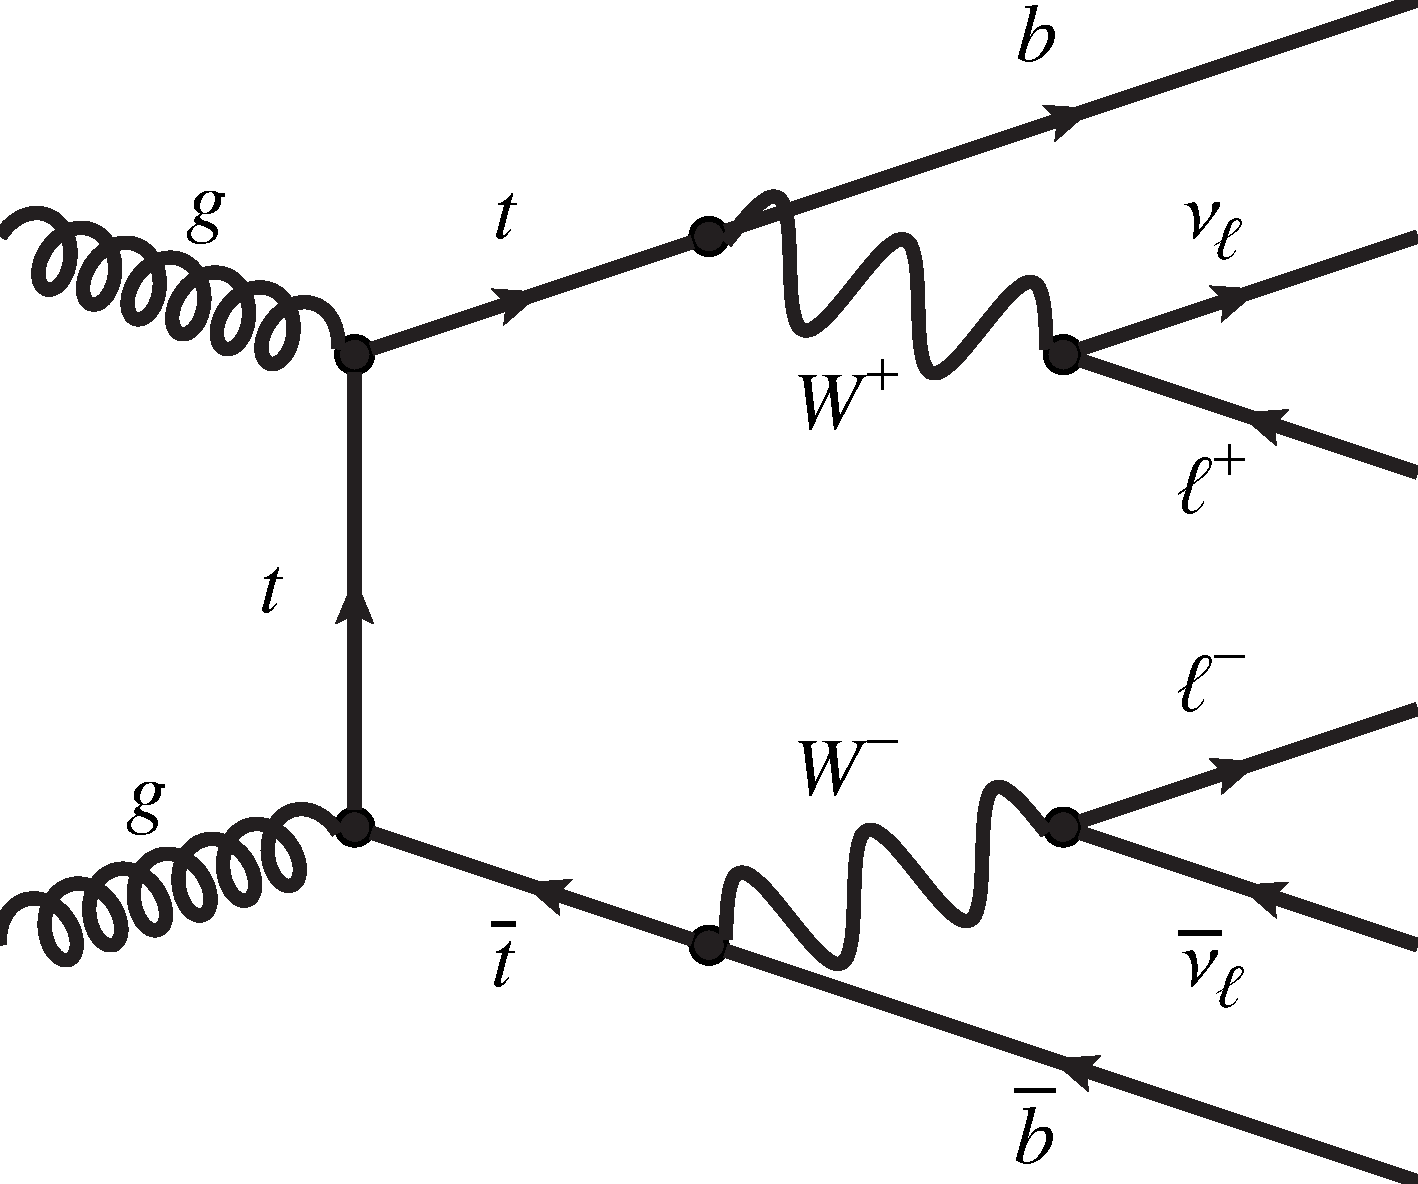
\includegraphics[width=\textwidth]{ttbar-decay}
        \caption{}
        \label{fig:nlo:ttbar}
    \end{subfigure}
\quad
    \begin{subfigure}[b]{0.44\textwidth}
        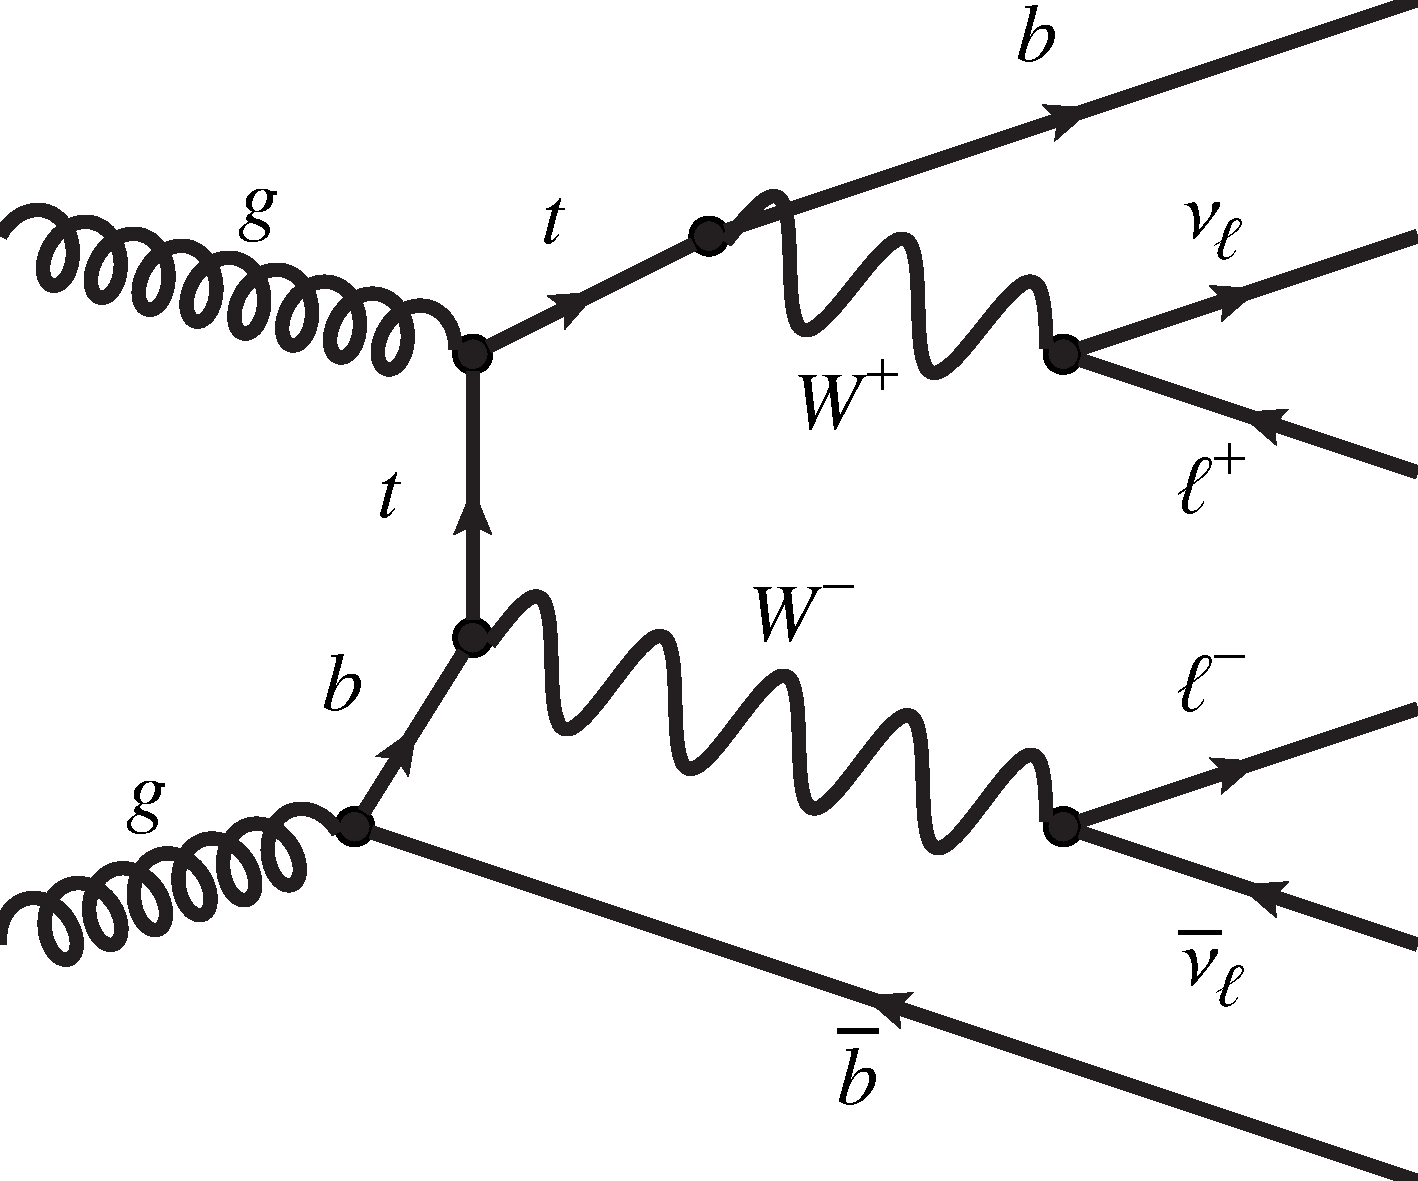
\includegraphics[width=\textwidth]{tw-NLO}
        \caption{}
        \label{fig:nlo:tw}
    \end{subfigure}
    \caption{}
	\label{fig:nlo}
\end{figure}
\chapter{Machine Learning}
\label{chp:ml}

\section{The concept of machine learning}

over the last decades computers have become indispensable tools of science, handling large amounts of data, completing tedious calculations and controlling sophisticated experiments. For the most part these  machines were assigned discrete tasks and they followed step-by-step commands designed beforehand by human users and had expected outcomes. 
For particle physics in particular, computers have been used to select and process data from large samples, allowing the processing of these data at a speed beyond human capabilities. However the selection rules always had to be generated by the user, therefore requiring an in depth understanding of the underlying system. In contrast machine learning enables a program to establish its own decision rules, improving these over several iterations and thereby learning to solve the problem by itself.

There has been a great effort over the last decades trying to implement a way for machines to learn from known quantities and thereby to enable them to analyse complex tasks ranging from voice recognition to object classification.
The efficiency and validity of a machine learning model is highly dependent on the human understanding of the problem at hand. One prerequisite for a successful model is the tuning of the degrees of freedom and parameters to the complexity of the assignment. This is called \emph{hyperparameter optimisation}, a task often proportional to the learning process itself.


Machine learning can be exemplified by drawing an analogy to human beings. In order to solve a problem, the machine needs to understand the system, to evaluate a decision step and finally generate new decision steps.
Understanding a system means to be aware of all its features and possibilities relevant to the task. Humans have their senses to easily break down their observations into useful features and concepts that can then be processed for finding a decision. A computer has no such senses and for most tasks this means that the step of filtering information for a relevant subset of features has still to be done by humans or a good preprocessing algorithm.
Once a system has been converted to a subset of features usable by a computer, the step of making its own decisions has to be implemented. This can be done by weighting and interconnecting the information using structures inspired by neurons and synapses in the human brain. 


The structure and complexity of the network enables it to learn from data. In addition, a metric is introduced that measures the quality of the model, called the \emph{cost} or \emph{loss function}. This function allows the network to improve iteratively as a decrease in its value is considered an improvement by the network. Combined with an optimiser which suggests further steps, this function is a basis for a network to independently approach a good decision rule for a incompletely investigated topic.

A very commonly used machine learning technique is the artificial neural network which on its own forms an extended field that builds the base of this work. The essential concepts of machine learning will be explained in the context of neural networks.

\section{Neural Networks}

The artificial neural network, or just neural network, is one of the most commonly applied approaches to machine learning. Its structure and naming is inspired by the neurons forming the human nervous system.

Instead of living neurons, a neural network consists of numerous very simple processors, called nodes.
 These nodes are usually structured into several layers as presented in fig (todo). In addition to that there are several ways to structure and connect these nodes frequently matching a certain problem. In this explanation only the most commonly way is explained. In that case each node of a layer is getting input from each node in the last layer and is outputting to each node of the following layer. Such a network structure is shown in figure \ref{fig:nodes_nomenclature} describing the step between a node and the previous layer. This is called a feed-forward neural network the math of which will be described in detail later.

\begin{figure}[htbp]
	\centering
	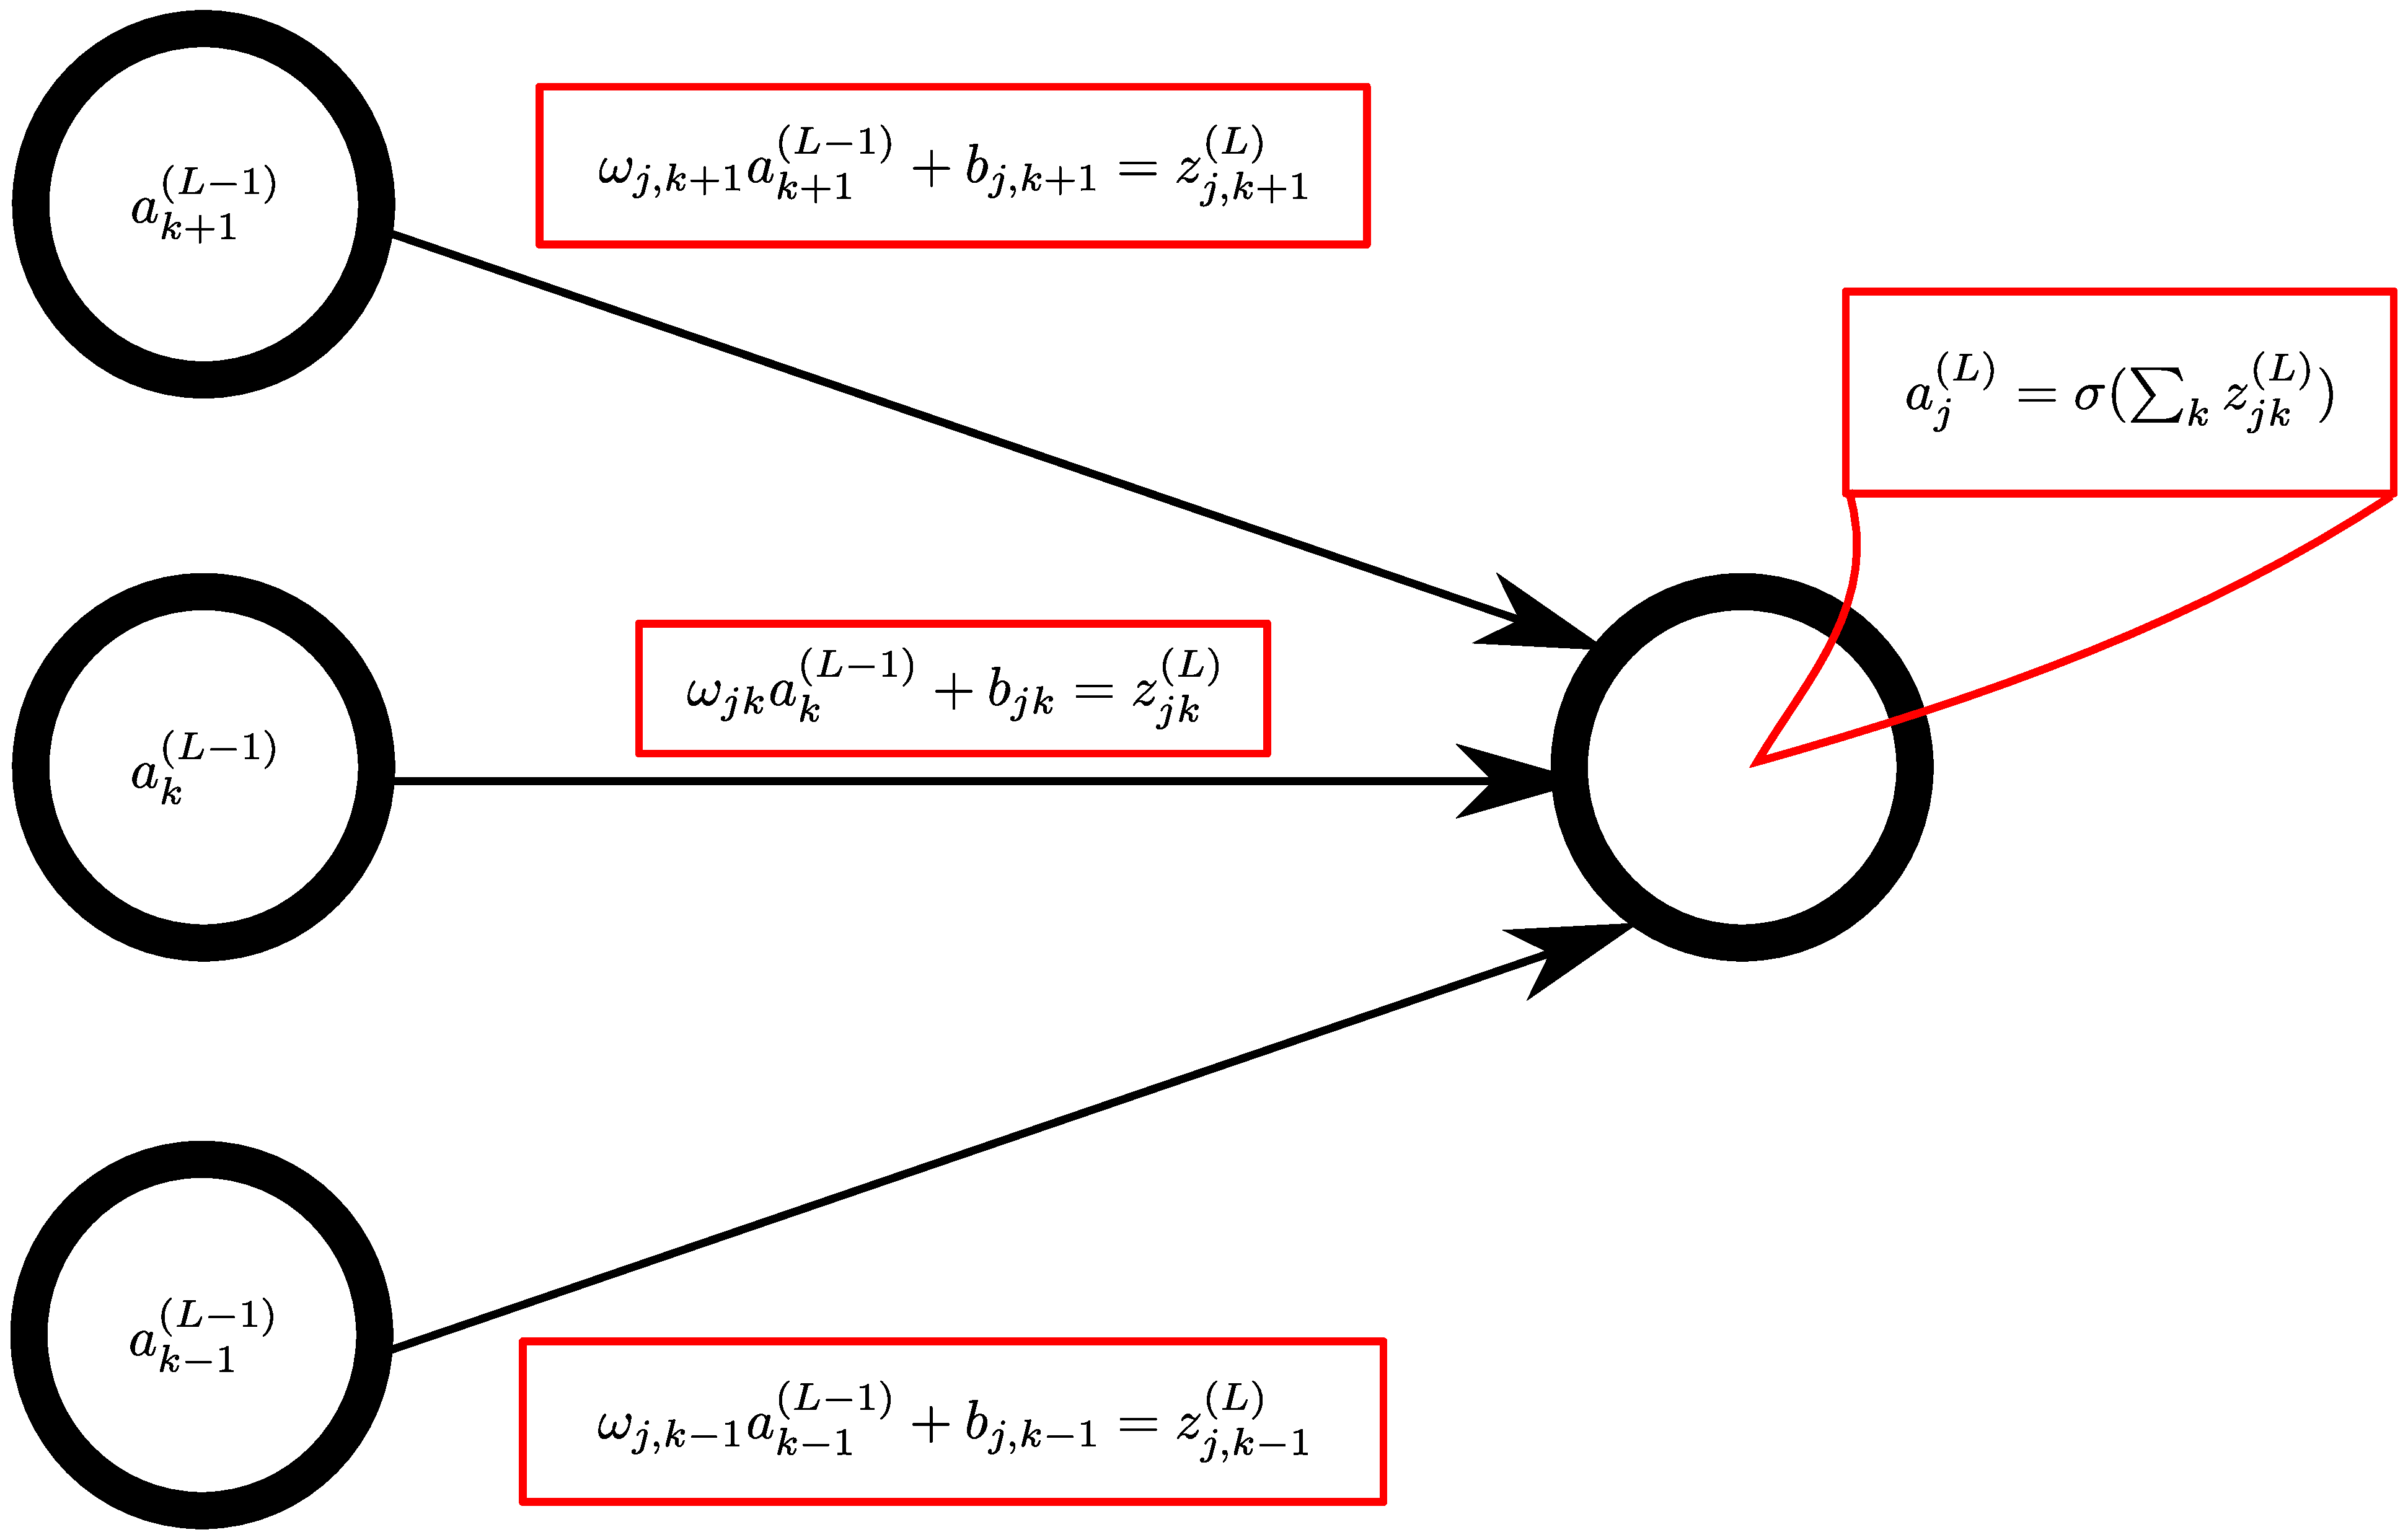
\includegraphics[scale=0.18]{figures_ML/nodes_nomenclature.eps}
	\caption[Network parameter nomenclature]{Network propagation from layer $(L-1)$ to layer $L$}
	\label{fig:nodes_nomenclature}
\end{figure}


\subsubsection{The input layer}

To understand a task and draw reasonable conclusions first the underlying system has to be understood which means its features need to be determined and summarised. The human brain is capable of investigating unknown systems and learning the features that are the most unique or interesting ones. For that the nervous system uses its senses to explore the system and process them later. To allow a machine to do something similar the unknown system has to be represented in a way that it is clear for the network what to look out for which is usually the task that requires most preprocessing by the user. The simplest case is to submit a list of variables to the network. In particle physics this could be kinematic variables of the final partons in an event.

The input to a neural network is just given to the input layer of nodes and subsequently processed through each following layer. For different tasks different layers might deal with different parts of the information but in this work the linear way of giving all information used to an input layer and then processing it is used.

\subsubsection{Decision making process}

Computers representing merely very powerful calculators, excel at performing high numbers of clearly defined calculations and therefore require a precisely elaborated task containing no uncertainty.

This is completely different for the human nervous system which relies on a certain uncertainty when processing information through a net of neuron cells where the output of every neuron is taken as input for the surrounding neurons. The challenge of machine learning is to represent this fuzziness by many somewhat discrete calculations. In the neural network the neurons and their fuzzy interaction is represented by the nodes which are very simple processors. Like neurons each node can use input from many other nodes to create a new output signal. Thereby the sets of input information can be linked to each other in numerous ways. Combined with a weighting system this allows to create complex models and match a variety of problems.

The input of every node is the weighted output of all previous nodes as shown in equation \eqref{eq:node_input}. $z_j^L$ is the input to the $j$-th node in the $L$-th layer. $\omega_{jk}^L$ is the weight from the $k$-th node in the previous layer to this node, $a_k^{L-1}$ is that node's output and $b_k$ the relevant bias, representing a possible intercept of the functionality. The sum indicates that all $k$ previous nodes contribute to the input to the $j$-th node.

\begin{align}
    z_j^L = \sum_{k=0}^{N} \omega_{jk}^L a_k^{L-1} + b_k
    \label{eq:node_input}
\end{align}


The weight allows to predict which variables are linked to each other or allow for better decision rules when combined but in addition to just define the strongest variables and features. Furthermore the output of each node is a non-linear combination of the input. This means the output can range from just one and zero to an exponential function and is called the activation function of a node. A common choice is the sigmoid function as presented in equation \eqref{eq:sigmoid_activation}.~\cite{chollet2015keras}

\begin{align}
    a_j^L = \sigma ( z_j^L ) = \frac{1}{1 + e^{z_j^L}}
    \label{eq:sigmoid_activation}
\end{align}

The sigmoid function has an output between \num{0} and \num{1} which is frequently desired for nodes especially for the final layer as we are looking for predictions of outcome probabilities. A selection of further activation functions is shown in table \ref{tab:activation_functions}.

\begin{table}[]
\centering
\begin{tabular}{l|l|l}

Name                    & Function & Plot \\ \hline
Sigmoid                 &$f(x) = \frac{1}{1 + e ^{-x}}$        &   \raisebox{-0.5\height}{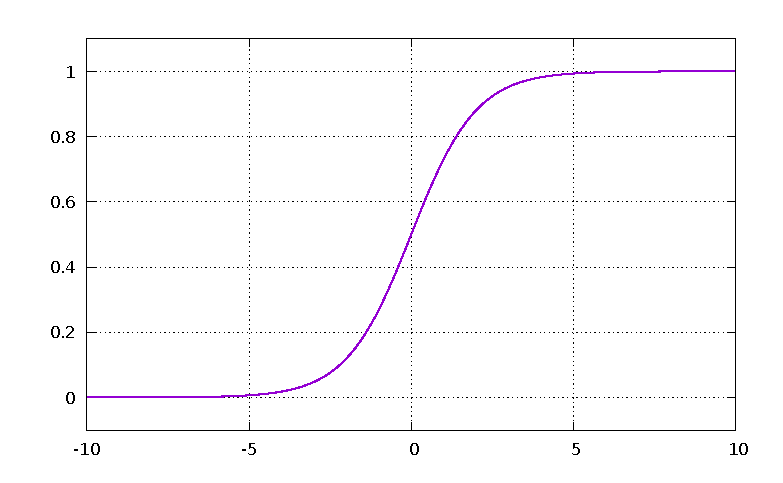
\includegraphics[scale=0.3]{figures_ML/sigmoid}}              \\ \hline
Tangens Hyperbolicus    &$f(x) = \frac{2}{1 + e ^{-2x}} -1$        &        \raisebox{-0.5\height}{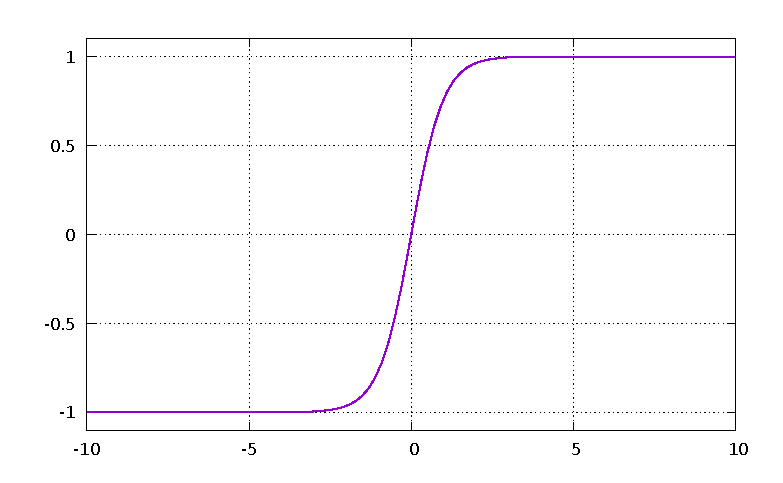
\includegraphics[scale=0.3]{figures_ML/tanh}}         \\ \hline
Rectified Linear Unit, \textsc{ReLu}   &$f(x) =
  \begin{cases}
    0       & \quad \text{if } x < 0\\
    x  & \quad \text{if } x \geq 0
  \end{cases}$     &      \raisebox{-0.5\height}{ 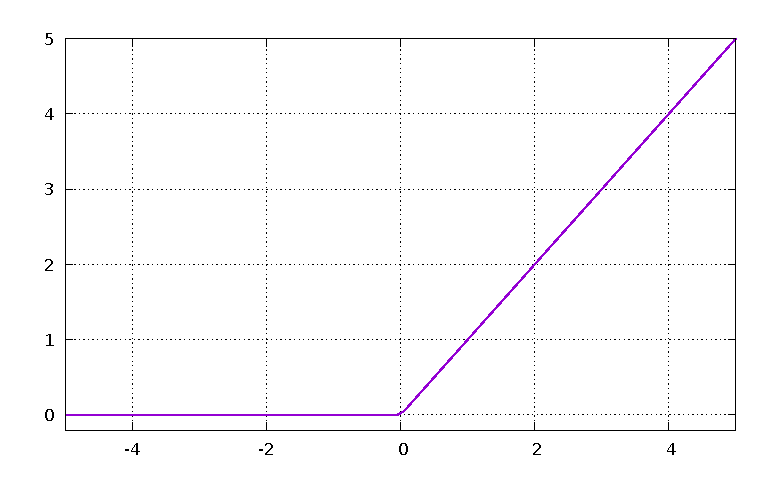
\includegraphics[scale=0.3]{figures_ML/relu}}          \\ \hline
Exponential Linear Unit, \textsc{ELU} &$f(x) =
  \begin{cases}
    \alpha ( e^x -1 )     & \quad \text{if } x < 0\\
    x  & \quad \text{if } x \geq 0
  \end{cases}$      &        \raisebox{-0.5\height}{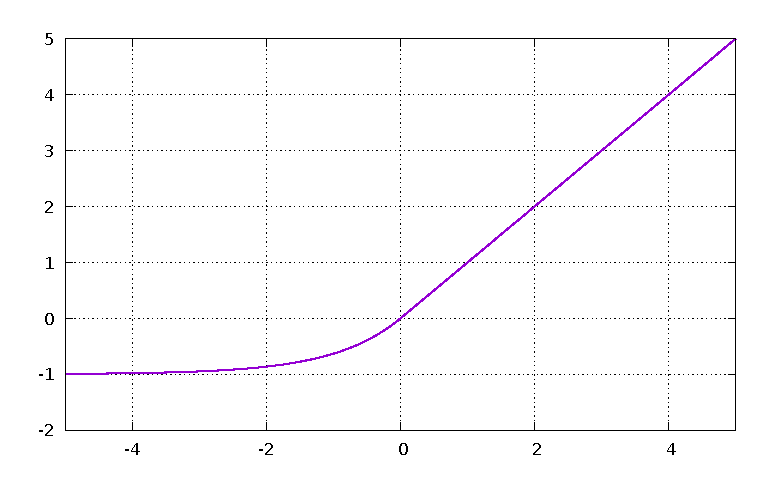
\includegraphics[scale=0.3]{figures_ML/elu}}         \\ 
\end{tabular}
\caption{Selection of activation functions taken from the Keras documentation. \cite{chollet2015keras}}
\label{tab:activation_functions}
\end{table}

For this thesis especially the exponential linear unit or \textit{elu} and the rectified linear unit or \textit{relu} were tested.
\textit{Elu} is suitable for converging the cost to zero rather fast and provides the possibility of negative output while \textit{relu} allows for the same benefit as sigmoid but  requires less computational power for the simply linear output for positive values.

Of course the network does still not know the task assigned to it but if we add a cost function to estimate the quality of a decision rule created by a certain combination of the input we can easily make the network approach a better decision rule in each step. Following the process of cost minimisation the solution of the initial problem can be approximated
In this work the cost function will be called the loss of the model.

In supervised learning the network is trained with a set of known data. Each event of the training set has a label representing the true outcome value referred to as just label or truth label. Comparing this truth information to the network output makes it very easy to calculate the loss as the deviation of the network output from the desired truth output. A possible loss function is the crossentropy or just binary crossentropy for a binary output result. As in this work the result is binary, signal and background, the binary crossentropy is the natural choice. Equation \eqref{eq:binary_crossentropy} shows the underlying function where $p$ is the estimated probability for the outcome $\hat{y}$ and $y$ is the label for a  correct or incorrect guess.

\begin{align}
    C = -(y \log p + (1 - y) \log (1 - p) )
    \label{eq:binary_crossentropy}
\end{align}

The loss is the most important indicator for the training quality. This quality must not be mixed up with the overall quality of the model as for the loss only the data trained on is taken into account but not a test data set.

\subsubsection{Optimizers - Choosing the next step}

The probability interaction of the nodes combined with the loss function enables a network not only to create a model but also to evaluate it. The last missing part is an algorithm that can estimate a step to a model that further minimises the loss. One could certainly do this randomly until the network finds a very low costed decision rule if infinite computational power was provided but that would neither be an efficient nor the desired learning process.

The output of each node in the final layer is defined by the weighted and biased information of the previous nodes and lastly the activation function. For one connection there are therefore three variables that have impact on the loss. Summarising this information for all nodes in a vector defines the loss-vector. The gradient of this vector is an estimator for the impact of each parameter on the overall loss and thereby gives a preferred direction for the model. Updating a network's parameters based on this gradient is called backpropagation. The algorithm works as follows:

\begin{enumerate}
    \item A certain set of input variables is iterated through all layers of a network resulting in an estimator $\hat{y}$ at each output node.
    \item The sum of deviations from the true value at all output nodes is determined as the loss $C$ of the setup. The loss just defines how good the model is.
    \item The gradient of the loss is calculated as the partial derivative of all network parameters
    \begin{align*}
        \frac{\partial C}{\partial a_k^{L-1}} = \sum_{j=1}^N \frac{\partial z_j^L}{\partial a_k^{L-1}} \frac{\partial a_j^L}{\partial z_j^L}\frac{\partial C}{\partial a_j^L}
    \end{align*}
    \item The parameters are then updated backwards through the layers following the negative loss gradient.
\end{enumerate}

This backpropagation algorithm is the backbone of the neural network's learning process.

The decision step based on the gradient defined above is specified by the networks optimizer and deserves a bit more attention. There are different choices of optimisers trying to accommodate different problems as well as some parameters important to understand and tune for an effective training. The length of a learning step has to match the problem's topology to properly let the model converge. First we define the gradient $g$ in a more general way. The batch size is $m$ and stands for the amount of data processed to evaluate the next step. $f$ is the network for a current configuration or model $\theta$ and the output $\hat{y}$. $\theta$ summarises all the parameters optimised by the network during the training. The output target provided by the truth information is $y$.

\begin{align}
    g = \frac{1}{m} \nabla_{\theta} \sum_j L(f(\hat{y}^j; \theta), y^i)
\end{align}

The configuration $\theta$ is then updated using the gradient and a constant $\eta$ called the learning rate as it determines the step size for each update.

\begin{align}
    \theta \prime = \theta - \eta g
\end{align}

Optimisation processes like this are gradient descent based optimisers and can be considered the basis of all optimisers. Depending on the choice they might be based on the whole training sample or just a mini batch of the sample. The most basic form has only learning rate as its hyperparameter. A good learning rate should be small enough to avoid oscillations but high enough to approach a minimum efficiently fast. A good estimate is given by the Robbins Monro condition:

\begin{align}
    \sum_k \eta_k = \infty\\
    \sum_k \eta_k^2 < \infty
\end{align}

As the choice of learning rate will not be perfect for every part of the problem's topology, momentum $\nu$ can be introduced as a second parameter to the optimizer.~\cite{chollet2015keras} The effect desired is to increase the step-size when the slope is long and the minimum is still far away and to decrease when approaching the minimum. Momentum scales each step by how aligned previous steps were meaning it will allow avoiding local minima or moving slowly along a slope by enlarging steps at the beginning of the training but it also will slow down at the end of the training when the steps become shorter. It promises to speed up the training with less risk of large oscillations which a large learning rate would probably result in. Momentum also takes a single scaling hyperparamter $\alpha$ and is updated each step following: 

\begin{align}
    \nu^{\prime} = \alpha \nu - \eta \frac{1}{m} \nabla_{\theta} \sum_j L(f(\hat{y}^j; \theta), y^j)\\
    \theta^{\prime} = \theta + \nu^{\prime}
\end{align}

Alternatively one can use Nesterov momentum~\cite{chollet2015keras} which is a more advanced adoption of momentum and updates the step a further time after applying the gradient: 

\begin{align}
    \nu^{\prime} = \alpha \nu - \eta \frac{1}{m} \nabla_{\theta} \sum_j L(f(\hat{y}^j; \theta + \alpha \times \nu), y^j)\\
    \theta^{\prime} = \theta + \nu^{\prime}
\end{align}

Finally it can be helpful to decrease the learning rate of the network stepwise while approaching a minimum to avoid oscillations or even missing the minimum completely. This can be accomplished by the hyperparameter of learning rate decay. It just decreases the learning rate in each iteration $t$ by a small hyperparamter $\phi$ following the assumption that smaller steps are sufficiently close to the minimum.~\cite{chollet2015keras}

\begin{align}
    \eta^{\prime} = \frac{\eta}{1 + \phi t}
\end{align}

\subsubsection{Adaptive optimisers}

In addition to the merely gradient based optimisers there are adaptive optimisers. Learning rate and momentum as previously described are difficult to tune to every part of the training process as the topology of the problem might rapidly change. Therefore adaptive optimisers update their parameters based on the training process. There is a set of adaptive optimisers.~\cite{chollet2015keras}\\
Often the adaptive optimiser of choice is \textsc{Adam}.~\cite{2014arXiv1412.6980K} \textsc{Adam} updates both, its learning rate and its momentum over the course of the training based on an exponentially decaying average of past gradients and past, squared gradients. The average makes sure that the parameters keep getting updated based on past steps. They should be decaying as otherwise the parameters would rapidly shrink. The decay of the averages is defined by a hyperparameter $\beta$.

\begin{align}
    \hat{g}^2 = \frac{\sum g^2}{1 - \beta_1^t}
\end{align}

\begin{align}
    \hat{g} = \frac{\sum g}{1 - \beta_2^t}
\end{align}

The model's parameters are then updated according to:

\begin{align}
    \theta^{\prime} = \theta + \frac{\eta}{\sqrt{\hat{g}^2} + \epsilon} \hat{g}
\end{align}

\textsc{Adam} is often considered a very good algorithm as it contains many corrections to hyperparamters during the training and thereby allows for easier optimisation but it also needs more computational power.


\section{Regularisation and Optimisation}

Fluctuations and noise in the training sample can be a big problem for a model trained on the sample as a neural network might pick noise and random fluctuations up as features of its decision rule which basically is the process of overfitting.

The network observes way more features to work with than those actually present in reality or even in a different test sample. The most extreme scenario is that your network is large and deep enough to pick up every single feature in the training sample. If that happens the training error becomes very low and indicates a very good decision rule. For a different sample this decision rule is at most very unreliable but probably strictly wrong resulting in a high test sample error. The network just picked up and remembered every single feature in the training sample instead of general correlations and thus becomes a mask of the sample.

A possible way to solve this issue is to stop the training early or to find a good way when to stop the training. This way noisy features might not yet have been picked up by the training. This might in turn also lead to a suboptimal result of the overall training as one cannot be sure that the correct features always get picked up first.

More sophisticated approaches are called regularisations of a neural network. The most commonly used solution is a so called Dropout layer described in the subsection \ref{sec:dropout}. Additionally a batch normalisation can have an effect of regularisation and is therefore introduced in this section as well.

\subsection{Dropout}
\label{sec:dropout}

Dropout can be introduced as an additional layer attempting to hinder the network from relying on less dominant features too much by removing different nodes in each iteration. This forces the network to build models that are not based on strong correlations between nodes making the weights become less interdependent. To simplify it significantly it means training several neural networks depending on which nodes are turned on during a training epoch which it keeps the training in motion for a large number of epochs.

Dropout is added to each layer of a network and can also be  restricted to a subset of layers. It slows down the training as the additional motion slows down the process of finding a minimum but it also accelerates each epoch slightly as it simplifies the network architecture. 

\begin{figure}[htbp]
	\centering
	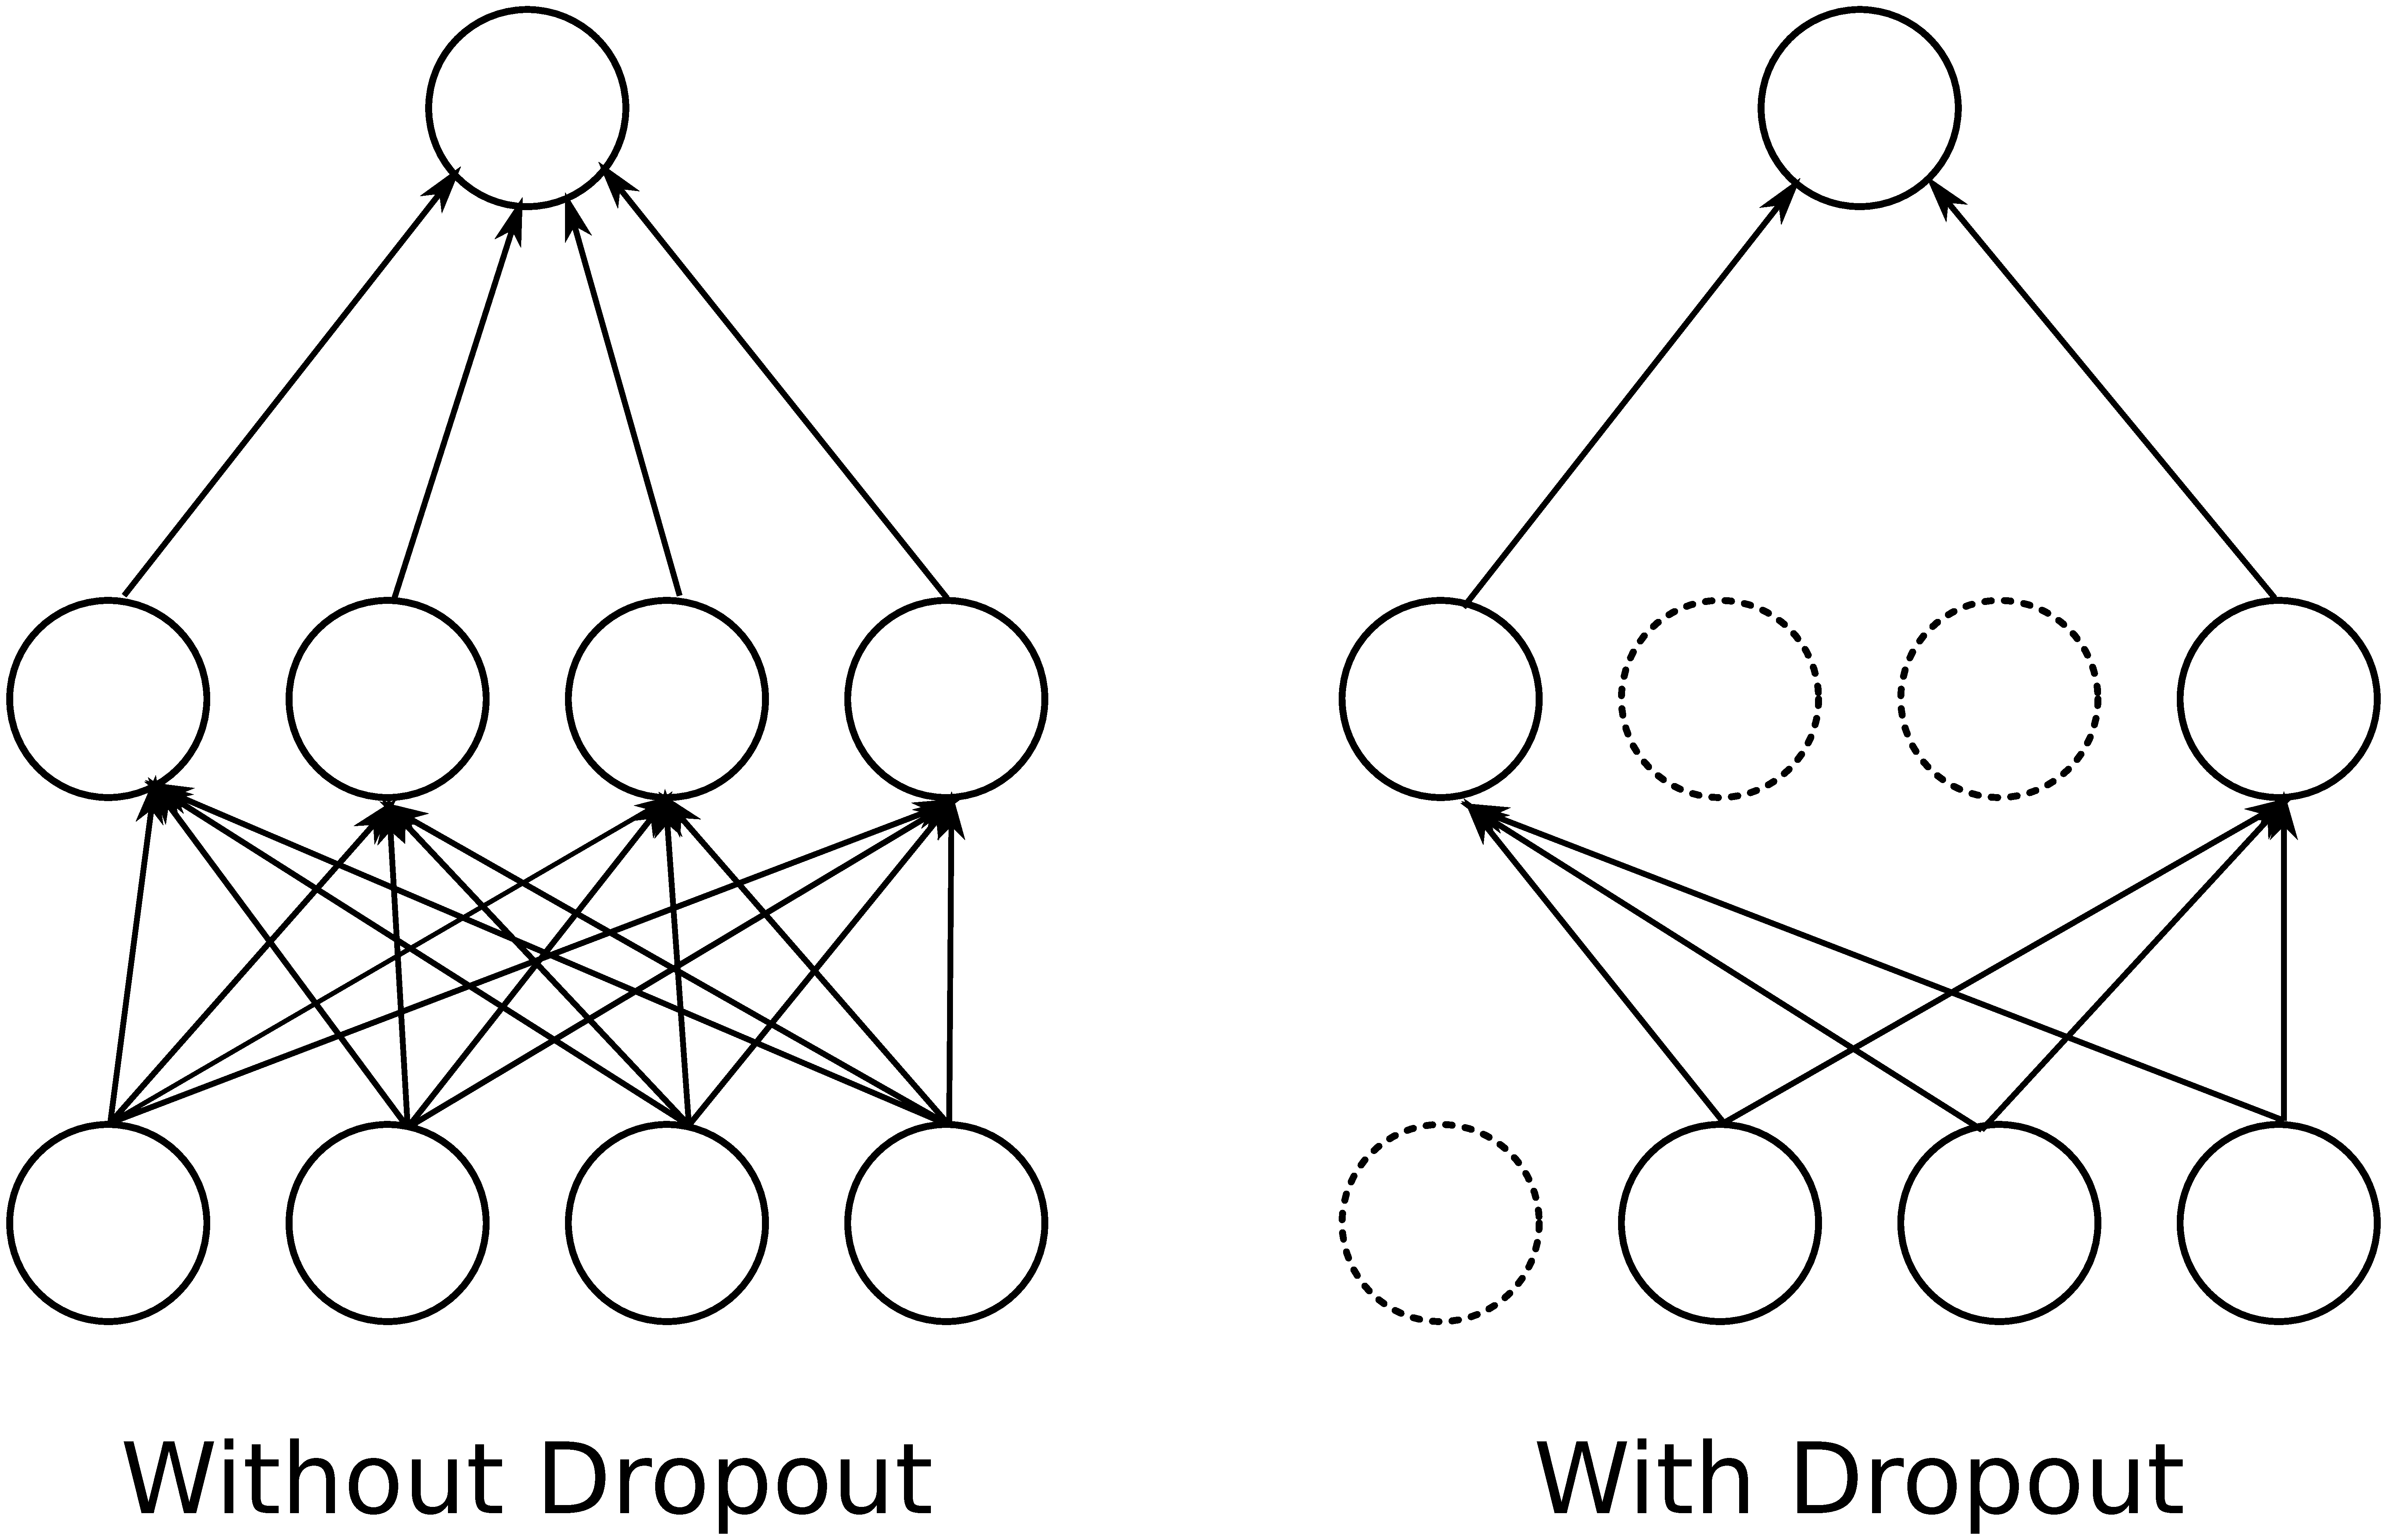
\includegraphics[scale = 0.1]{figures_ML/dropout.eps}
	\caption[Dropout Sketch]{Sketch of network before and after the inclusion of dropout. On the left hand side dropout is not applied and all nodes are connected. On the right hand side the dashed circles are nodes excluded by dropout and therefor not connected to the other nodes.}
	\label{fig:dropout}
\end{figure}



\subsection{Batch normalization}
\label{sec:batch_norm}

In supervised learning the training result is strongly dependent on the set of data the network is trained on. This means that the performance might change dramatically when the test data is very different. Imagine a classifier distinguishing between pictures that show cars and pictures that do not show cars. If the training set contains predominantly green cars the colour green might end up as a strong indicator for  the classification car. In general the colour green will not be as dominant and the network will perform slightly worse when trying to classify cars of a different colour. Formally such a change of input is called a covariance shift.

A way to reduce the effect of covariance shift is batch normalization. The output of nodes in general and the weight of a connection in a neural network is not necessarily limited allowing for certain connections to be really dominant and overshadowing less dominant features. We want to avoid this as the dominance of some features might just be present in the training sample. This can be achieved by normalizing the output of each layer in the network to the total output and thereby minimising the effects of strongly overrepresented features. This is done by normalizing each output to the mini-batch mean $\mu_B$ and the mini-batch standard deviation $\sigma_B^2$.

\begin{align}
    \mu_B = \frac{1}{m} \sum_i x_i\\
    \sigma_B^2 = \frac{1}{m} \sum_i (x_i - \mu_B)^2\\
    x_{i,norm} = \frac{x_i - \mu_B}{\sqrt{\sigma_B^2 + \epsilon}}
\end{align}





\section{Adversarial Neural Networks}

This main part of this work is the examination and training of an adversarial neural network. An adversarial neural network consists of a classifier and a second network that tries to regularise the output of the first classifying network.

In this section the concept of an adversarial neural network is motivated and the underlying mathematics as originally stated in paper~\cite{2014arXiv1406.2661G} are presented.
For more information about an approach directly tested on physics see the paper "Learning to Pivot with Adversarial Networks".~\cite{Louppe:2016ylz}

\subsection{The adversarial neural network}

Neural networks have been very successful in classifying tasks but less successful for generative tasks. This was the original problem that gave birth to the idea of a generative adversarial network. Generative networks often produce output that is very easy to distinguish from real samples. The solution suggested is adding a classifier that tries to distinguish between generated samples and real samples. As long as this adversary is able to accomplish this task the first network fails at its generative task. Training the two networks against each other disincentives the generative network from using the features not dominant in real samples.

In this work the first network is not a generator but a classifier separating signal events from background events in a Monte Carlo simulation. These simulations contain systematic uncertainties and different samples represent a set of plausible data generation processes. The classifier should not be too dependent on variables with high systematic uncertainties as the network cannot account for differences in the training and testing sample or even in real data. If the classifier has these strong dependencies on systematic uncertainties it might lead to a high co-variance shift.

Instead of a generated sample and a truth sample, a so called nominal sample and systematic samples are used as input for the second network. Systematic samples have slightly different distributions than the original samples because of changes to the variables with the systematic uncertainties. Training the second network on determining whether it is looking at a nominal or a systematic sample allows to estimate how strongly the model depends on variables with high systematic uncertainties. Training the classifier against the adversarial network promises to reduce the effect of systematic uncertainties on the model. If the topology of the problem allows for it this should render the model generated by the classifier pivotal. That means it does not depend on the unknown values of the nuisance parameters.

Mathematically this comes down to a minimax decision rule or a competition between two neural networks. Let us call the classifier $Net1$ and the adversary $Net2$ then the problem becomes:

\begin{align}
    \min_{Net1} \max_{Net2} V(Net1, Net2) = \mathbb{E}_{\mathit{x} \sim \rho_{data}} [ log Net1(\mathit{x}) ] + \mathbb{E}_{\mathit{z} \sim \rho_{sys}} [ log (1 - Net2(\mathit{z}) ) ]
\end{align}

$V(Net1, Net2)$ is the combined value function for the two adversary networks. The first network is trained to be an optimal classifier represented by $log Net1(\mathit{x})$ while the second network is trained to distinguish between the nominal and systematics distribution $\mathit{z} \sim \rho_{sys}$ represented by $log (1 - Net2(\mathit{z}))$.

 In theory the first classifier should be trained slowly and kept close to its optimum while the second network slowly learns and allows the first network to adapt to it. This is achieved by training the two networks successively over multiple iterations using a combined value function.
As this value function a combined loss function is used. It is just the difference between the two separate loss functions with a hyperparameter $\lambda$ to control the impact of the adversary as shown in equation \eqref{eq:adversarial_loss}.

\begin{align}
    \mathcal{L} = L_{net1} - \lambda L_{net2}
    \label{eq:adversarial_loss}
\end{align}

In the first step of each iteration the first network is trained using the combined loss function $\mathcal{L}$. In the second step the second network is trained using its simple loss function $\lambda L_{net2}$. Each of the networks has the usual set of hyperparameters to optimise explained in detail in the previous sections missing.

In this work the adversarial network is set up by building a classifying network. The information of the classifier is then fed into both the classifier's output layer and the adversarial network creating a second model based on the first network's model. The networks are then trained successively controlling the combined and separate losses. Figure \ref{fig:ANN_sketch} shows a sketch of the setup.

\begin{figure}[htbp]
	\centering
	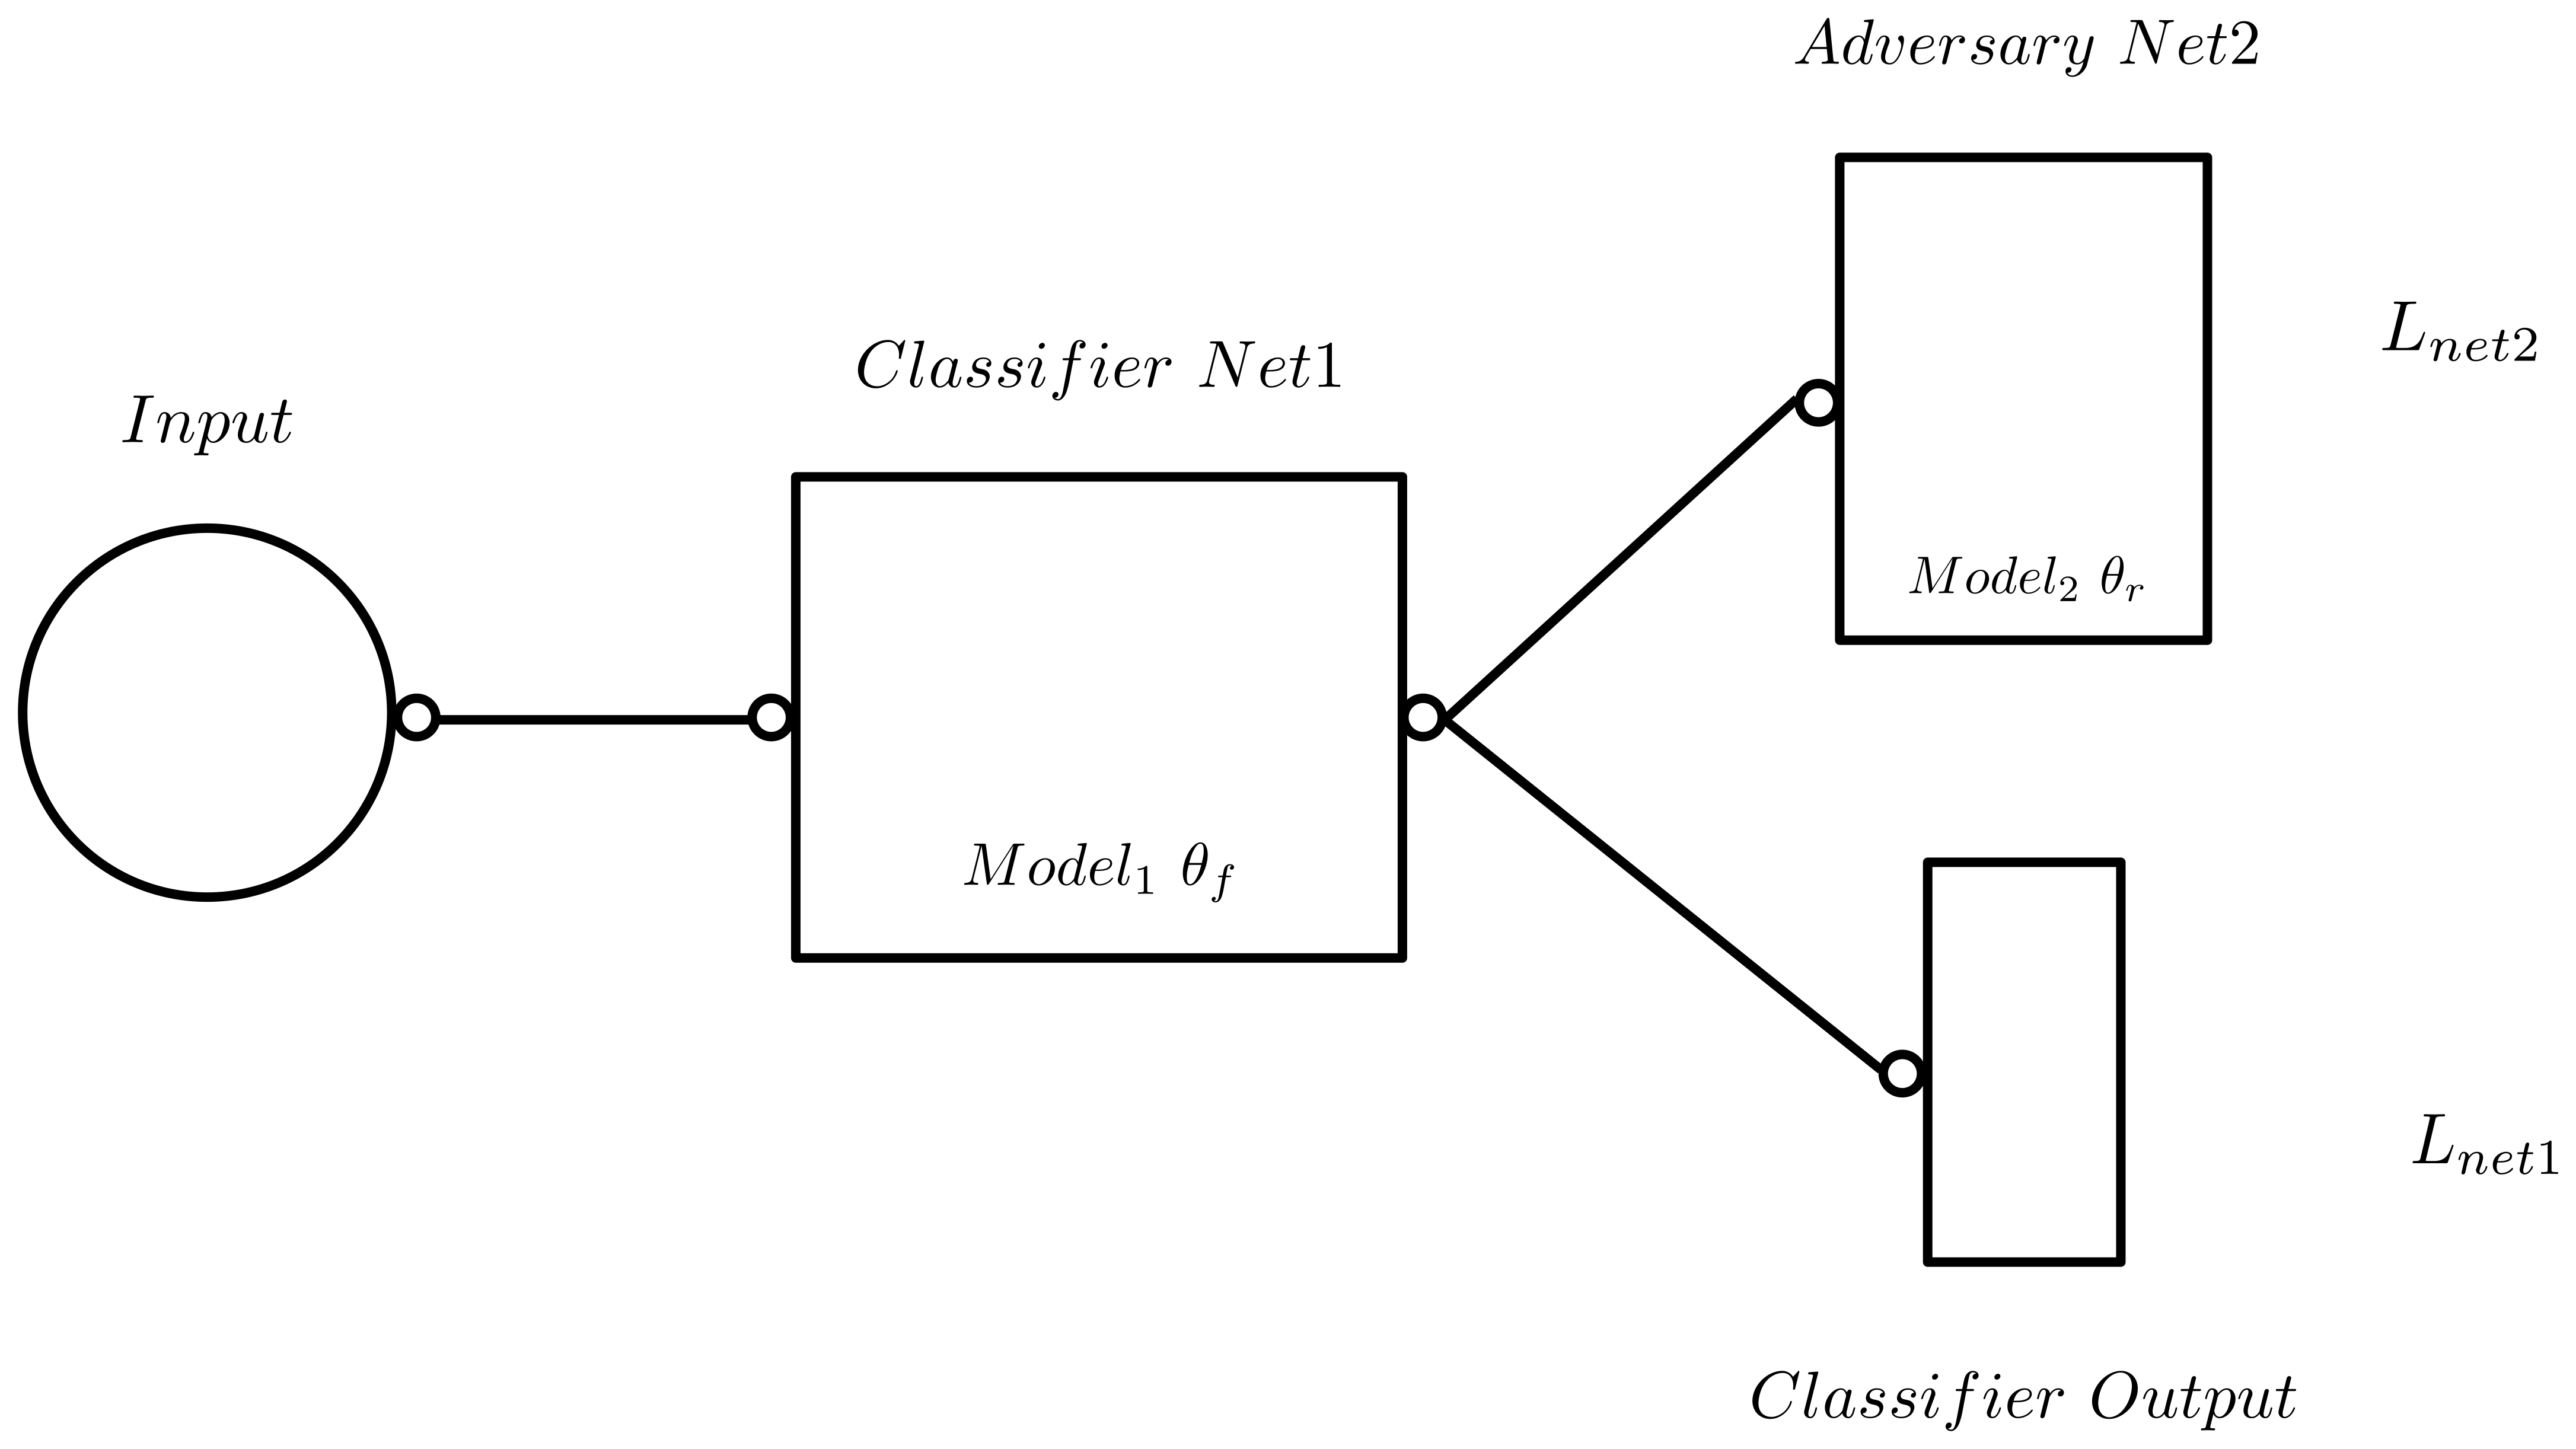
\includegraphics[width=0.9\textwidth]{figures_ML/ANN_sketch.png}
	\label{fig:ANN_sketch}
	\caption[Adversarial setup sketched]{Sketch of the network setup. The main part is the classifier. The model generated is fed into both the second network and the classifier's output. This way the two losses $L_{net1}$ and $L_{net2}$ are generated. Furthermore the training of the classifier immediately affects both output models.}
\end{figure}

The hyperparameter $\lambda$ is set to tune the impact of the second network on the model. A large $\lambda$ leads to a very pivotal model but can also decrease the overall quality of the classifier.

In order to better understand the figures shown in chapter \ref{chp:ANN} the three loss values of an adversarial neural network will be introduced as the last part of this chapter.
The first loss belongs to the classifier and is expected to first increase as the adversary finds a good model and to decrease once a more pivotal model is found. 
The second loss displays the adversary's performance ideally decreasing at first to then increase and saturate as a pivotal model renders it impossible to extract any information.
Lastly the combined loss is displayed showing the overall performance and decreasing as good models are found for both the classifier and the adversary.
Figure \ref{fig:losses_paper} shows an example for this loss functions taken from the paper "Learning to Pivot with Adversarial Networks".~\cite{Louppe:2016ylz}

\begin{figure}[htbp]
	\centering
	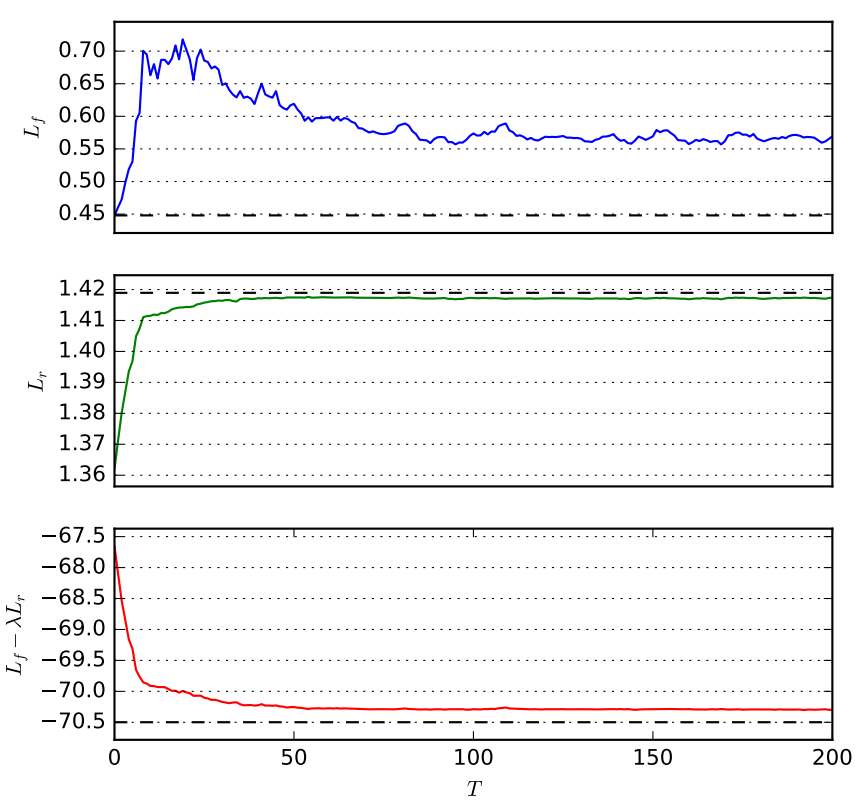
\includegraphics[width=\textwidth]{figures_ML/losses_paper}
	\caption[Exemplary loss of an adversarial network structure]{Three losses of an adversarial network for $\lambda = 10$ taken from a toy example.~\cite{Louppe:2016ylz} From top to bottom the classifier, adversary and combined loss is presented. $T$ is the number of training iterations.}
	\label{fig:losses_paper}
\end{figure}




\chapter{Hyperparameter optimisation of a classifying neural network}
\label{chp:simpleNN}

The adversarial neural network is based on a common classifying neural network trained on signal/background separation. The output of that network is then used as input for the adversary to create a negative back-feed for the classifier.
Before the adversarial, second network is added, the classifying network is optimised on its own to make sure that its setup is sufficient for the classification task.
During the adversarial training this setup can be updated if the structure is not optimised for the additional task of a model that is less sensitive to systematic uncertainties.

This chapter describes the hyper-parameter optimisation of the first network starting with the motivation of the input information.
The second section explains the choice of the architecture followed by the step-wise setup of the optimiser.
Lastly regularisation of the network is tested and described.
The overall aim of the description is to provide some understanding on the hyper-parameters available and their correlations. The impact of the hyper-parameters on the training results is presented not only to introduce their function but also to motivate possible solutions later on.

To train the network and to test its performance all its parts need to be in place. Therefore all hyper-parameters had to be initialized with values assumed to represent a good setup. Initially this was accomplished by starting with a very simple network using a minimal set of hyper-parameters which were then elaborated to a more and more optimised network. The results shown in this work are going to be based on the final choice of hyper-parameters where only one parameter is then varied at a time to explain the impact of the particular tuning. Sometimes this leads to the effects of a hyper-parameter to be less strong. The already optimised model is more stable, and if no significant impact is visible the plots are not shown. For that reason section~\ref{sec:simplesetup} will already introduce the final network structure, which is then step by step to be explained and motivated.

The structure was achieved within reason and the computational power constraints. There certainly are hyper-parameters that deserve more attention and in addition to that there are alternative setups for the whole network that were not tested. A further investigation of network optimisation is without a doubt very promising.


\section{Technical details}
\label{sec:technicals}

The artificial neural networks in this thesis were created using the Keras python library~\cite{chollet2015keras}.
Keras is an application programming interface written in python and able to run on Tensorflow, CNTK or Theano. It was developed by google and summarizes the necessary calculations for running a deep neural network training in fast and easy modules.
The backend is the package responsible for the underlying vector calculations needed for the network setup and training. In this work the Tensorflow package was used as a backend~\cite{tensorflow2015-whitepaper}.

\section{Final setup of the network}
\label{sec:simplesetup}

This section describes the fully optimised classifier which is then parameter-wise varied during this chapter to motivate the particular choices.
The hyperparamters are listed and the loss curve, the ROC curve and the final separation are shown in figure~\ref{fig:simple:final}. They are the main tools a training performance is evaluated on in this thesis. For the sake of completeness the agreement between nominal and systematic response is also shown as it will be a standard inclusion for the plots during the adversarial training.


\begin{itemize}
\item Input: \num{14} variables motivated by a BDT variable scan.
\item Hidden layers: \num{6} \ELU layers $\times$ \num{128} nodes each
\item Output layer: \num{1} \SIGMOID node
\item Optimisation: SGD, Learning rate $=0.06$, momentum $=0.3$, no nesterov, no decay
\item Duration: 600 epochs
\end{itemize}

\begin{figure}[htbp]
    \centering
    \begin{subfigure}[b]{0.48\textwidth}
        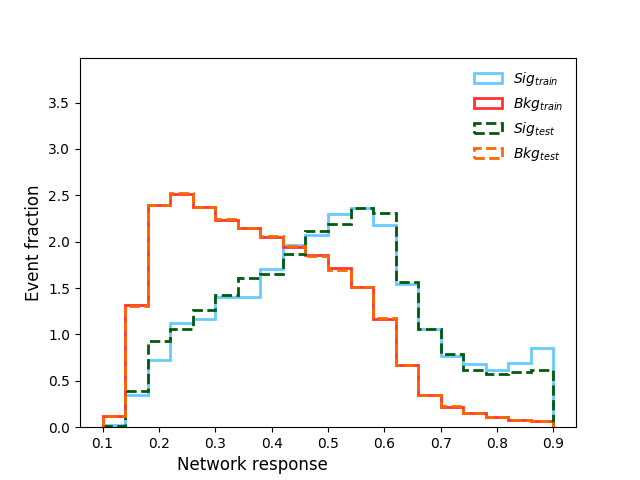
\includegraphics[width=\textwidth]{standard_separation}
        \caption{}
        \label{fig:simple:final:sepa}
    \end{subfigure}
\quad
    \begin{subfigure}[b]{0.48\textwidth}
        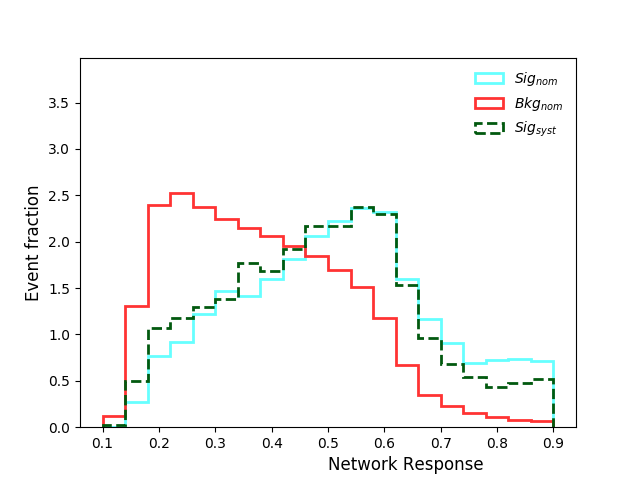
\includegraphics[width=\textwidth]{standard_syst}
        \caption{}
        \label{fig:simple:final:syst}
    \end{subfigure}

    \begin{subfigure}[b]{0.48\textwidth}
		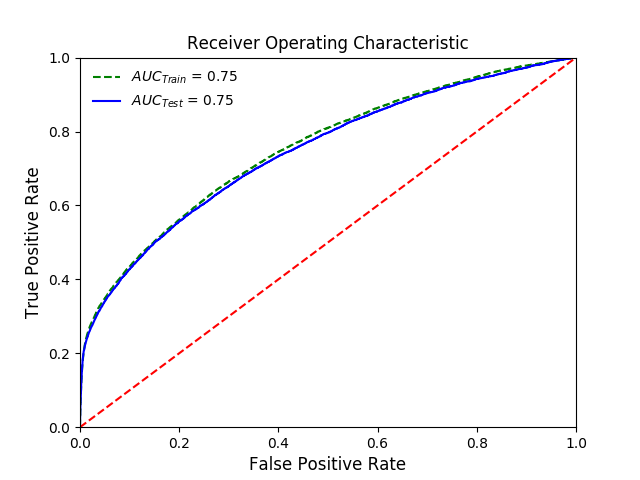
\includegraphics[width=\textwidth]{standard_ROC}
		\caption{}
		\label{fig:simple:final:roc}
	\end{subfigure}
\quad
	\begin{subfigure}[b]{0.48\textwidth}
		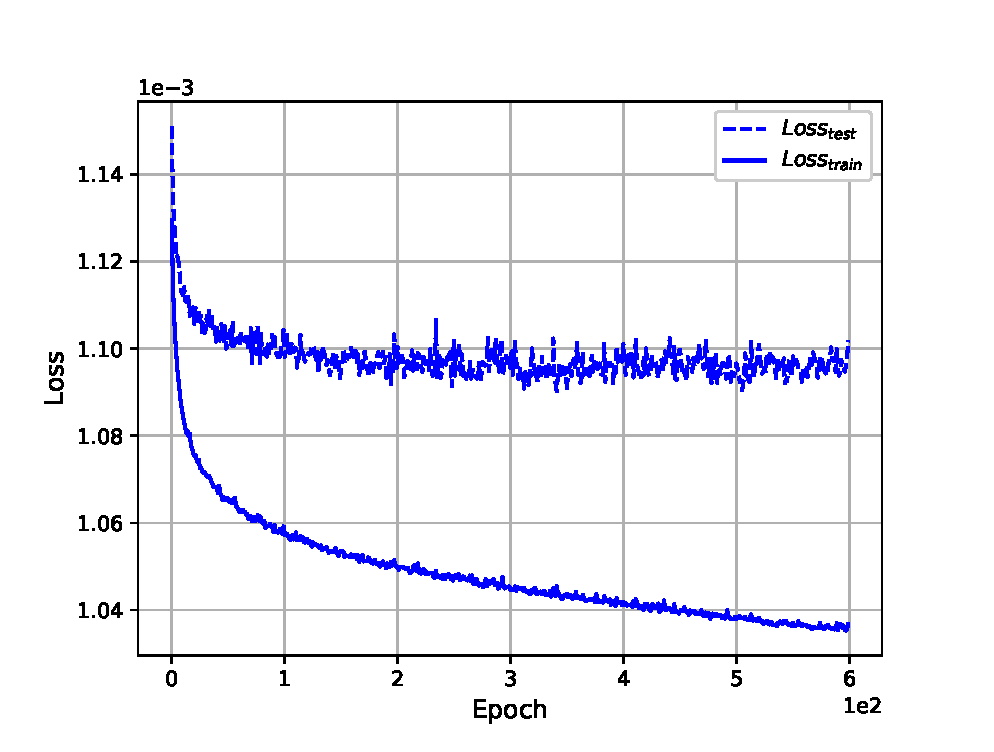
\includegraphics[width=\textwidth]{standard_losses}
		\caption{}
		\label{fig:simple:final:loss}
	\end{subfigure}
    \caption[Network performance of the classifier]{Figure~\subref{fig:simple:final:sepa} shows the response of the classifier. The solid lines represent the training sample and the dashed lines the test sample. Figure~\subref{fig:simple:final:syst} shows the difference for response in systematic and nominal samples. The solid lines represent the nominal samples and the dashed line the systematic sample. Figure~\subref{fig:simple:final:roc} shows the ROC curve. The dashed line is the training curve and the solid line is the test curve. Figure~\subref{fig:simple:final:loss} diagrams the losses with dashed for test and solid for training.}
	\label{fig:simple:final}
\end{figure}


\section{The input variables}

Two sets of input variables were tested for the classifier.
The first one is a set of simple kinematic variables. This is tested to exploit a neural network's ability to deduce all further information from the complete basis of a system.
The second set of variables uses more complex variables based on the most significant variables for a boosted decision tree usage on the same problem.
The variable sets used were:
%
%
%
\begin{table}[h]
    \begin{minipage}{.5\linewidth}
      \caption{}
      \centering
		\begin{tabular}{l|l}
		Variable                              & Branch                            \\
		\pTmiss                & met                               \\ \hline
		$|\eta_{jet1}|$ & absEta\_Jet1 \\ \hline
		$|\eta_{jet1}|$ & absEta\_Jet2 \\ \hline
		$|\eta_{lep1}|$ & absEta\_Lep1 \\ \hline
		$|\eta_{lep2}|$ & absEta\_Lep2 \\ \hline
		${\pT}_{jet1}$  & pT\_jet1    \\ \hline
		${\pT}_{jet2}$    & pT\_jet2     \\ \hline
		${\pT}_{lep1}$    & pT\_lep1     \\ \hline
		${\pT}_{lep2}$    & pT\_lep2     \\ \hline
		$\phi_{jet1}$   & phi\_jet1    \\ \hline
		$\phi_{jet2}$   & phi\_jet2    \\ \hline
		$\phi_{lep1}$   & phi\_lep1    \\ \hline
		$\phi_{lep2}$   & phi\_lep2    \\ \hline
		\end{tabular}
    \end{minipage}%
    \begin{minipage}{.5\linewidth}
      \centering
        \caption{}
		\begin{tabular}{l|l}
		\hline
		Variable & Branch                        \\ \hline
		$m_{lep1} + m_{jet2}$									& mass\_lep1jet2                \\ \hline
		         & pTsys\_lep1lep2met            \\ \hline
		         & pTsys\_jet1jet2               \\ \hline
		$m_{lep1} + m_{jet1}$									& mass\_lep1jet1                \\ \hline
		${\pT}_{lep1} - {\pT}_{jet1}$							& deltapT\_lep1\_jet1           \\ \hline
		${R}_{lep1} - {R}_{jet2}$								& deltaR\_lep1\_jet2            \\ \hline
		         & deltaR\_lep1lep2\_jet2        \\ \hline
		$m_{lep2} + m_{jet1}$									& mass\_lep2jet1                \\ \hline
		${\pT}_{jet2}$											& pT\_jet2                      \\ \hline
		${R}_{lep1} - {R}_{jet1}$								& deltaR\_lep1\_jet1            \\ \hline
		${R}_{lep1} - {R}_{jet1}$		& deltaR\_lep1lep2\_jet1jet2met \\ \hline
		${R}_{lep2} - {R}_{jet2}$								& deltaR\_lep2\_jet2            \\ \hline
		$\text{Centrality}_{lep2} + \text{Centrality}_{jet2}$	& cent\_lep2jet2                \\ \hline
		${R}_{lep2} - {R}_{jet1}$		& deltaR\_lep2\_jet1            \\ \hline
		\end{tabular}
    \end{minipage} 
\end{table}
%
Figure \ref{fig:vars} shows a comparison of the separation and the loss curves for both variable sets. It is visible that for the set of simple variables the network runs into overtraining after about \num{200} epochs visible in plot~\ref{fig:vars:simple:loss} because \losstrain and \losstest start to diverge. This also results in a bad separation with a strong disagreement between the two samples. There is an argument for testing a simple set of variables for a shorter training duration. However, this optimisation process would be a project of its own. Furthermore, in this work one has to keep in mind that the network is supposed to be used in adversarial setup later. This demands for a longer training period and a large number of good features to be available. Otherwise the probability of finding a classifier, less sensitive to a systematic uncertainty, decreases and the behaviour of the losses has to supervised very carefully.

Showing an overall good performance the set of complex variables as suggested by the boosted decision tree variable scan performed in the analysis \enquote{Measurement of the cross-section for the production of a \PW boson in association with a top quark at \SI{13}{\tera \electronvolt}} was chosen\cite{Finelli:2667560}. Please note that the set of variables in the paper referred to does not fully agree with the variables used in this work. The reason being that the variables were adopted while the research was still ongoing.

\begin{figure}[htbp]
    \centering
    \begin{subfigure}[b]{0.45\textwidth}
        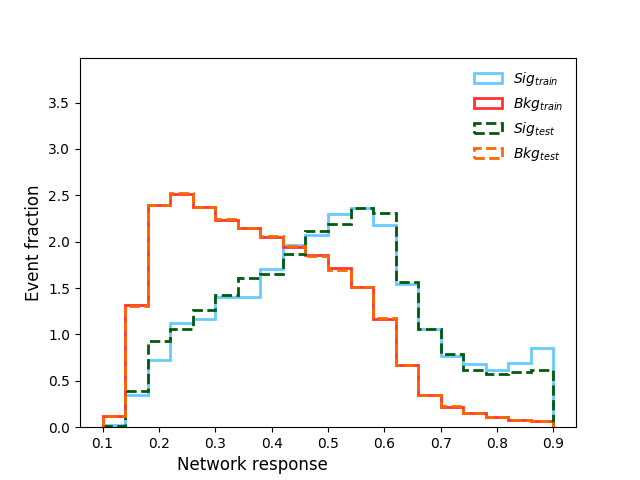
\includegraphics[width=\textwidth]{standard_separation}
        \caption{}
        \label{fig:vars:standard:sep}
    \end{subfigure}
\quad
    \begin{subfigure}[b]{0.45\textwidth}
        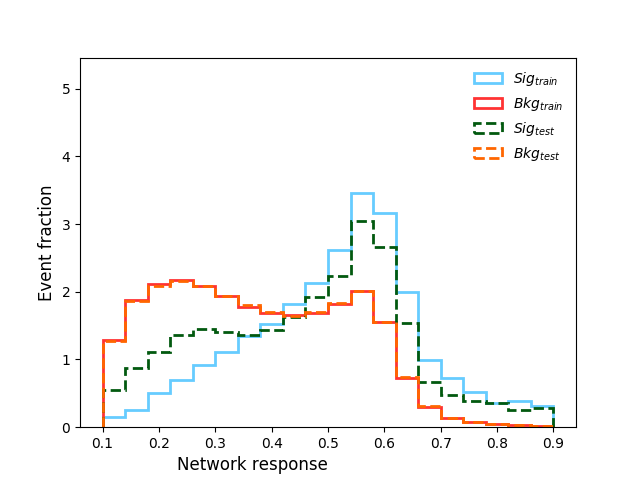
\includegraphics[width=\textwidth]{simple_vars_separation}
        \caption{}
        \label{fig:vars:simple:sep}
    \end{subfigure}

    \begin{subfigure}[b]{0.45\textwidth}
		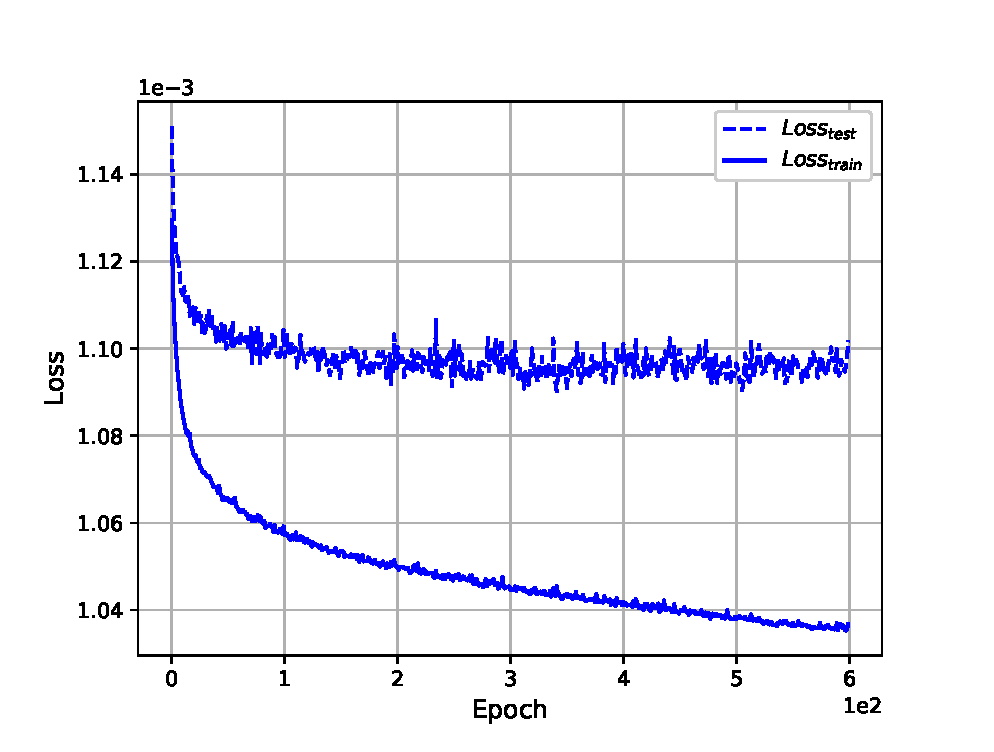
\includegraphics[width=\textwidth]{standard_losses}
		\caption{}
		\label{fig:vars:standard:loss}
	\end{subfigure}
\quad
	\begin{subfigure}[b]{0.45\textwidth}
		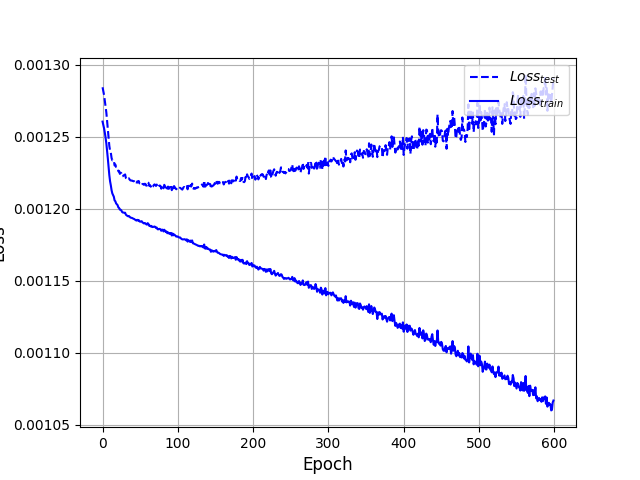
\includegraphics[width=\textwidth]{simple_vars_losses}
		\caption{}
		\label{fig:vars:simple:loss}
	\end{subfigure}
    \caption[Performance of the classifier using different variables]{Figure~\subref{fig:vars:standard:sep} and figure~\subref{fig:vars:simple:sep} show the separation for the complex and simple variables respectively. The losses for the variable sets are diagrammed in figure~\subref{fig:vars:standard:loss} and figure~\subref{fig:vars:simple:loss}.}
	\label{fig:vars}
\end{figure}





\section{The network architecture}

The architecture of the neural network is formed by its nodes and layers. The choice of the architecture is nontrivial and, as a lot of aspect's of machine learning, not an exact science.
However, one can make some assumptions about the appropriate architecture.
First of all the complexity of the model should about match the complexity of the task assigned. Although it usually is not trivial to find an estimator for a task's complexity and even less to match it to a certain architecture, a test series often leads to a good estimate. Another possible starting point is the amount of variables necessary to fully describe a system resulting in the minimum variable number necessary to input in the network. This also gives a first estimate on how large the architecture should at least be.
Both the depth and the overall size of the model play a role. A simplified way of explaining these two properties is by saying that the depth defines how often the input is processed while the number of nodes is the number of features that can be kept during each step of processing.

In general an architecture that is too deep and wide will pick up too many features too fast. That means it overtrains before it finds a good minimum. This can be seen in an early divergence between the training loss and the test loss. An architecture too simple is not able to pick up the features of the task at all resulting in no learning process. The loss stays constant or changes very slowly.

In this work a test-series was performed, training a network for a wide range of combinations of nodes and layers; $\text{nodes}\in[8:512]$ and $\text{layers}\in[1:10]$. For the sake of simplicity the number of nodes per layer was kept constant during each training. Two variables were then plotted against the size of the architecture. First the overall smallest loss the model achieved during the training was plotted. The other variable was the minimal difference between the training and the test loss. To keep it simple the complexity of the architecture was defined as the product of nodes and layers. These are certainly not the most sophisticated indicators for the model's complexity and its performance. However, the plots do allow for some sophisticated guesses for a good choice of architecture.

Figure~\ref{fig:minimal_loss} shows that more complex architectures also achieve smaller loss values. This unfortunately is not a clear sign for an overall good performance as heavily overtrained networks will achieve low loss values as well. Therefore, a second estimator was taken into account. Figure~\ref{fig:minimal_diff} shows the minimal difference between \losstrain and \losstest achieved during the whole training process. There are two regions showing a small difference. The first is the region of very simple architectures. This however, is a result of a slow learning process. No features are being picked up that differentiate between the two sets used for loss evaluation. The second region, \numrange{500}{800}, was used as the region of choice, before heavy overtraining occurs. Finally, a more complex architecture in this region, comprising \num{6} layers with \num{128} nodes each, was chosen. Although this choice seems fairly arbitrary at this point, there is arguments for a complex architecture as it can always be regulated using dropout if need be. Additional prove that further increasing the architecture leads to overtraining can be gained by looking at the loss for a complex architecture in figure~\ref{fig:complex_arch}. Here the overtraining becomes visible in the difference between the two curves and their overall odd behaviour.



\begin{figure}[htbp]
    \centering
    \begin{subfigure}[b]{0.45\textwidth}
        \centering
        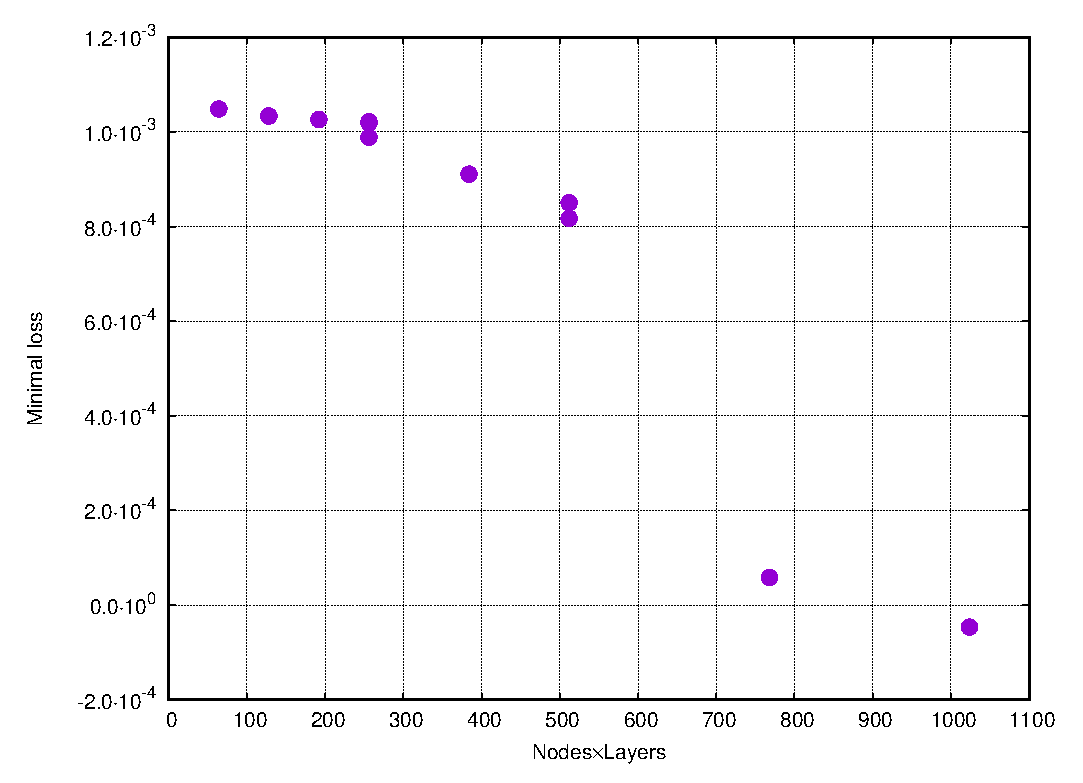
\includegraphics[width=\textwidth]{figures_simpleNN/minimal_loss.eps}
        \caption{Minimal loss}
        \label{fig:minimal_loss}
    \end{subfigure}%
\quad
    \begin{subfigure}[b]{0.45\textwidth}
        \centering
        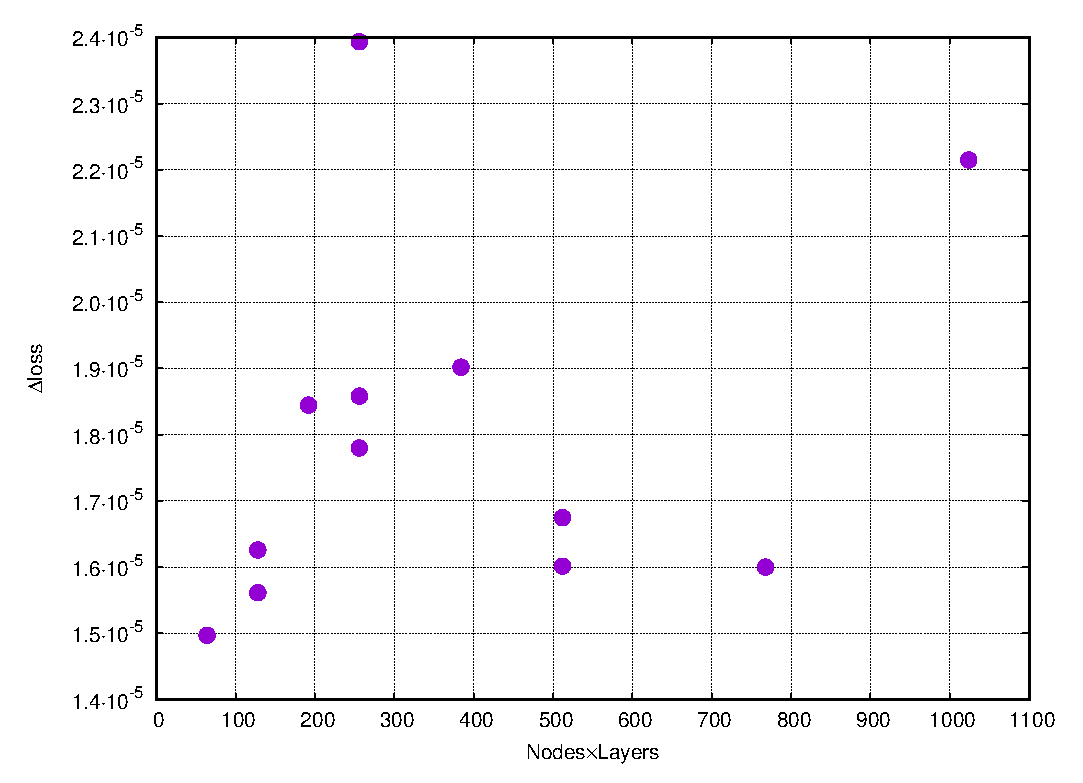
\includegraphics[width=\textwidth]{figures_simpleNN/minimal_diff.eps}
        \caption{Minimal loss difference}
        \label{fig:minimal_diff}
    \end{subfigure}
    \caption[Network performance's dependency on the architecture]{Figure~\subref{fig:minimal_loss} shows the minimal overall loss achieved during the training for the range of architectures. Figure~\subref{fig:minimal_diff} shows the minimal difference between \losstrain and \losstest achieved.}
    \label{fig:net_complexity}
\end{figure}



\begin{figure}[htbp]
	\centering
	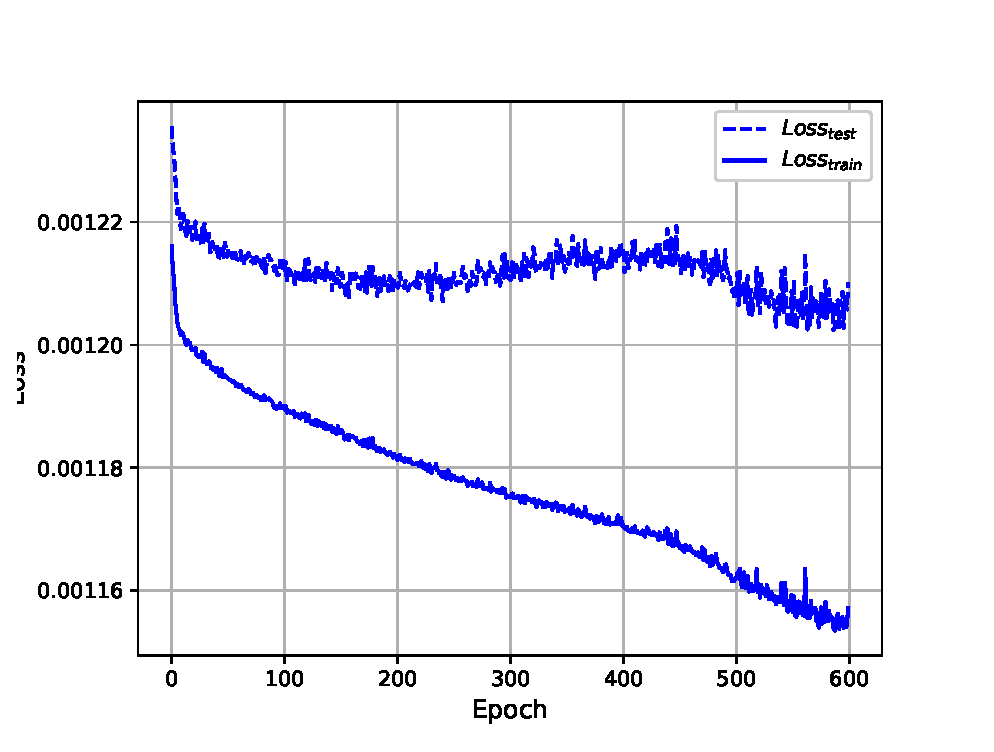
\includegraphics[width=0.8\textwidth]{complex_arch_losses}
	\caption[Classifier losses for a complex architecture]{Loss function for the classifier for \num{8} layers and \num{512} nodes each.}
	\label{fig:complex_arch}
\end{figure}

In addition to the choice of the architecture the activation function for the layers has to be set.
Two different activation functions come to use in the neural network. The main function connects the nodes in the hidden layers while the last one converts the output to a value between \num{0} and \num{1}. For the output the sigmoid function is a natural choice and no other activations were tested.
For the hidden layers \ELU and \RELU were tested. Figure~\ref{fig:activ} shows a comparison of the ROC curve and the loss development for both activation-functions. For \RELU a strong disagreement between training- and test-sample occurs and \ELU became the activation function of choice. Further activation-functions were not tested due to time constraints.

\begin{figure}[htbp]
    \centering
    \begin{subfigure}[b]{0.48\textwidth}
        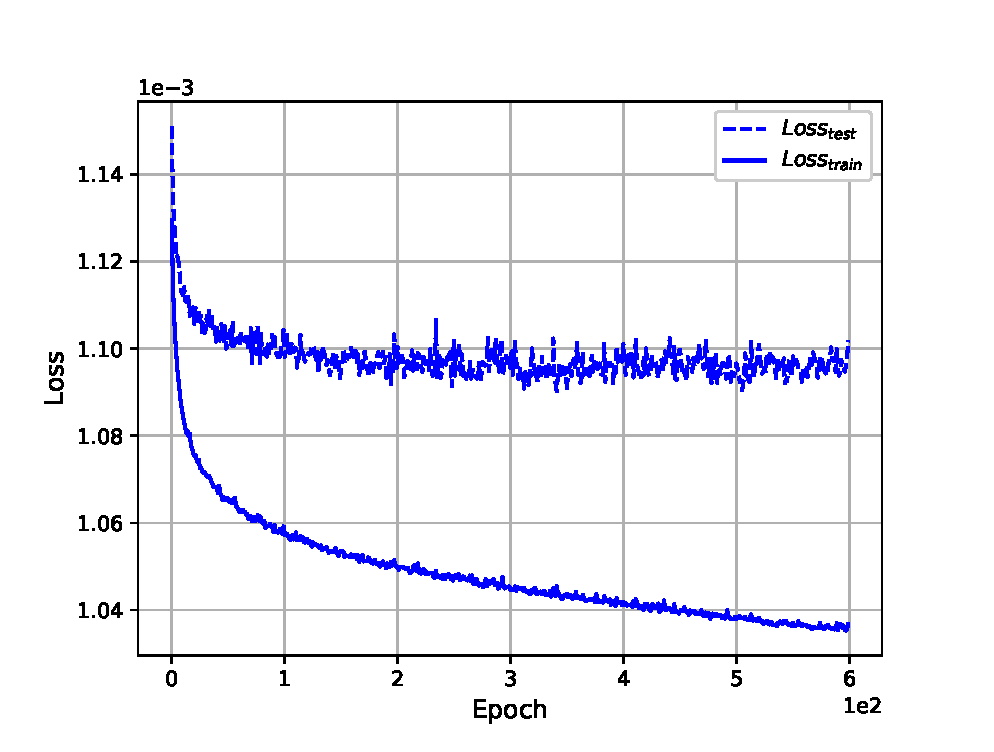
\includegraphics[width=\textwidth]{standard_losses}
        \caption{}
        \label{fig:activ:standard:loss}
    \end{subfigure}
\quad
    \begin{subfigure}[b]{0.48\textwidth}
        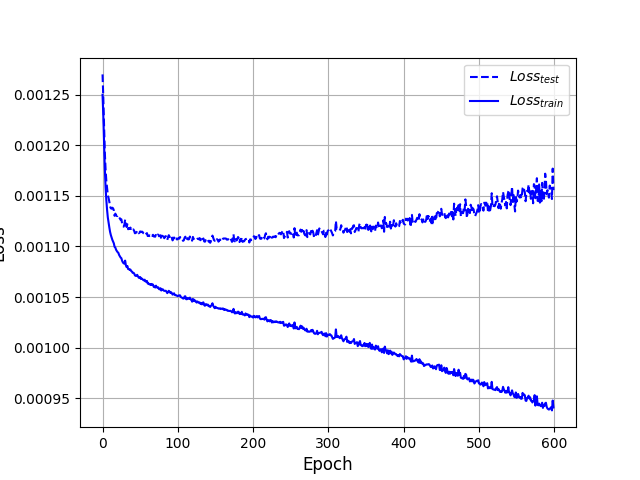
\includegraphics[width=\textwidth]{relu_losses}
        \caption{}
        \label{fig:activ:relu:loss}
    \end{subfigure}

    \begin{subfigure}[b]{0.48\textwidth}
		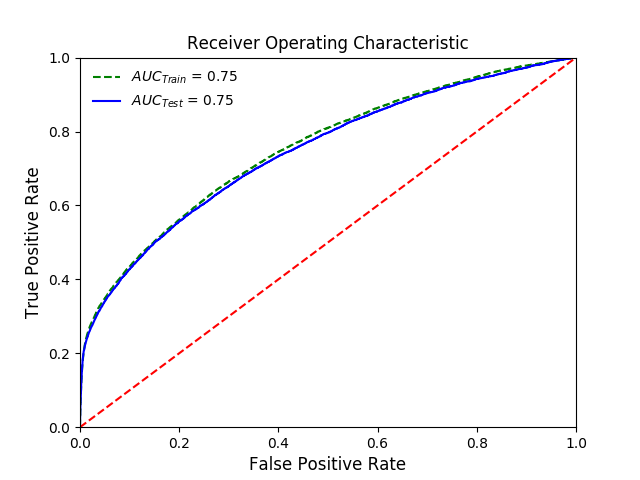
\includegraphics[width=\textwidth]{standard_ROC}
		\caption{}
		\label{fig:activ:standard:roc}
	\end{subfigure}
\quad
	\begin{subfigure}[b]{0.48\textwidth}
		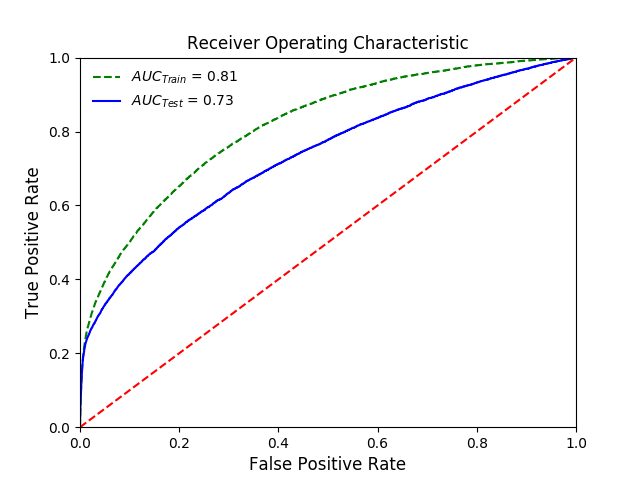
\includegraphics[width=\textwidth]{relu_ROC}
		\caption{}
		\label{fig:activ:relu:roc}
	\end{subfigure}
    \caption[Classifier performance for different activation functions]{Figure~\subref{fig:activ:standard:loss} and figure~\subref{fig:activ:relu:loss} show the losses for \ELU and \RELU respectively. The ROC curves for the different activation-functions are diagrammed in figure~\subref{fig:activ:standard:roc} and figure~\subref{fig:activ:relu:roc}.}
	\label{fig:activ}
\end{figure}


\section{Setup of the optimisation}

For the most part of the optimisation SGD was used as the optimiser and its tuning is shown in detail.
Adam was also tested out but not fully tuned, due to constraints on time and computational resources.
In subsection~\ref{sec:optimiser:choice} a brief overview of the performance using Adam is given. Section~\ref{sec:optimiser:tuning} describes the fine tuning of the SGD optimiser in more detail.

\subsection{Choice of the optimiser}
\label{sec:optimiser:choice}

A classic gradient-based optimiser, SGD, is compared to the adaptive optimiser, Adam. Figure~\ref{fig:opti} compares the loss development for both optimisers. It is obvious that Adam behaves strangely and it was therefore discarded. It is possible that Adam could outperform SGD for a better tuning of its hyper-parameters and it certainly is worth testing out if the computational power is provided.

\begin{figure}[htbp]
    \centering
    \begin{subfigure}[b]{0.48\textwidth}
        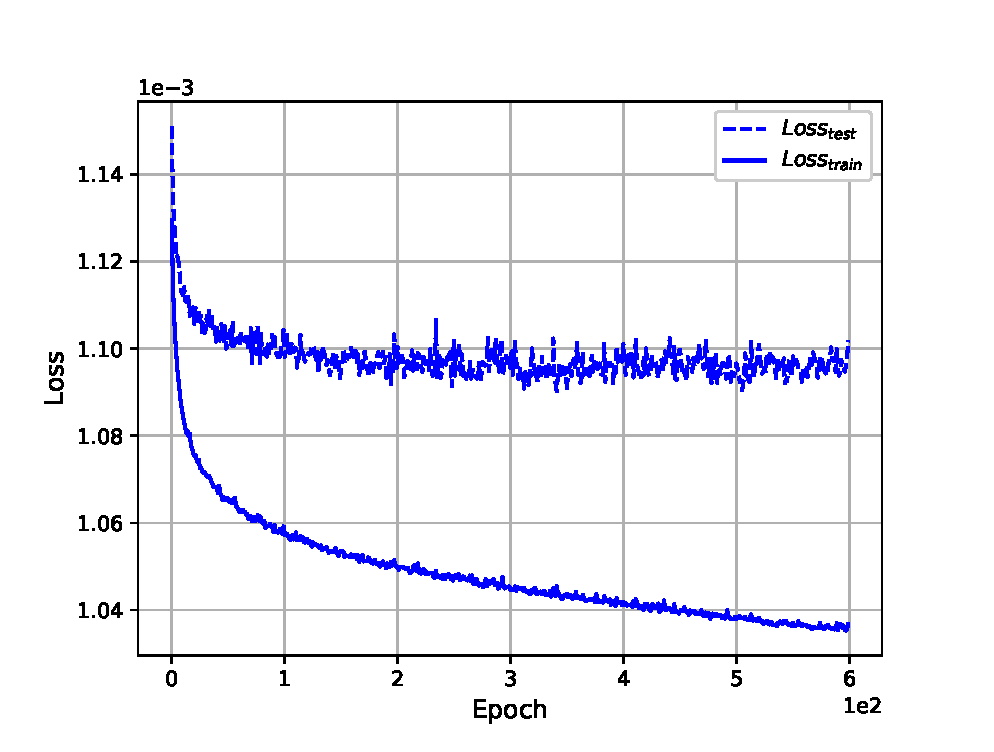
\includegraphics[width=\textwidth]{standard_losses}
        \caption{}
        \label{fig:opti:standard}
    \end{subfigure}
\quad
    \begin{subfigure}[b]{0.48\textwidth}
        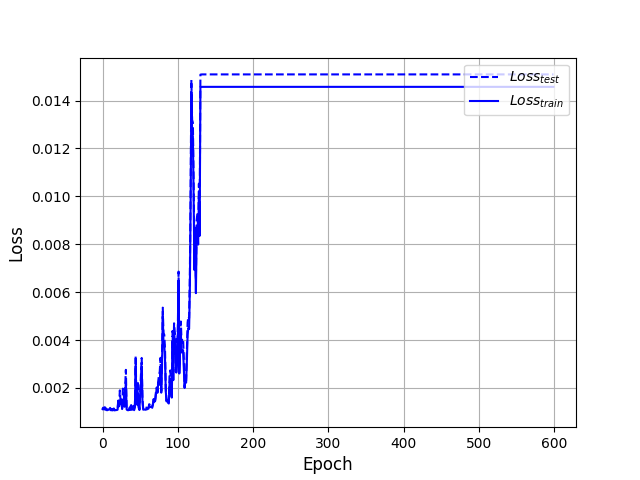
\includegraphics[width=\textwidth]{adam_losses}
        \caption{}
        \label{fig:opti:adam}
    \end{subfigure}
    \caption[Classifier losses for different optimisers]{Loss curves for SGD~\subref{fig:opti:standard} and Adam~\subref{fig:opti:adam}.}
	\label{fig:opti}
\end{figure}

\subsection{Tuning the optimiser}
\label{sec:optimiser:tuning}

As described in section\ref{sec:optimisation} an optimiser has several hyper-parameters of its own. In this section the learning rate, the momentum with the option of Nesterov, and the decay parameter will be probed.
For the learning rate a range of values between a small learning rate of \num{0.001} and high learning rates up to \num{0.5} were tested to investigate the behaviour. The choice was based on how high the oscillations are and how efficiently the training converges. High learning rates were discarded for an increased probability of overtraining and a lot of unwanted oscillations while small learning rates made the training unnecessarily slow and inefficient. Figure~\ref{fig:lr} shows a comparison of the network losses for a small learning rate of \num{0.001}~\ref{fig:lr:small} and a relatively large learning rate of \num{0.2}~\ref{fig:lr:large}. For the small learing rate there are no signs of overtraining and no oscillations visible. However, the training converges slowly. For a high learning rate the \losstrain and \losstest show larger divergence and each curve shows more oscillations individually. In the end an intermediate learning rate of \num{0.06} is chosen.

\begin{figure}[htbp]
    \centering
    \begin{subfigure}[b]{0.48\textwidth}
        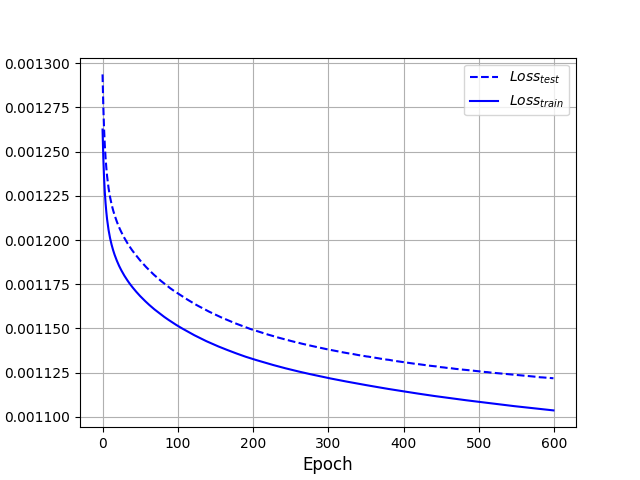
\includegraphics[width=\textwidth]{smalllr_losses}
        \caption{}
        \label{fig:lr:small}
    \end{subfigure}
\quad
    \begin{subfigure}[b]{0.48\textwidth}
        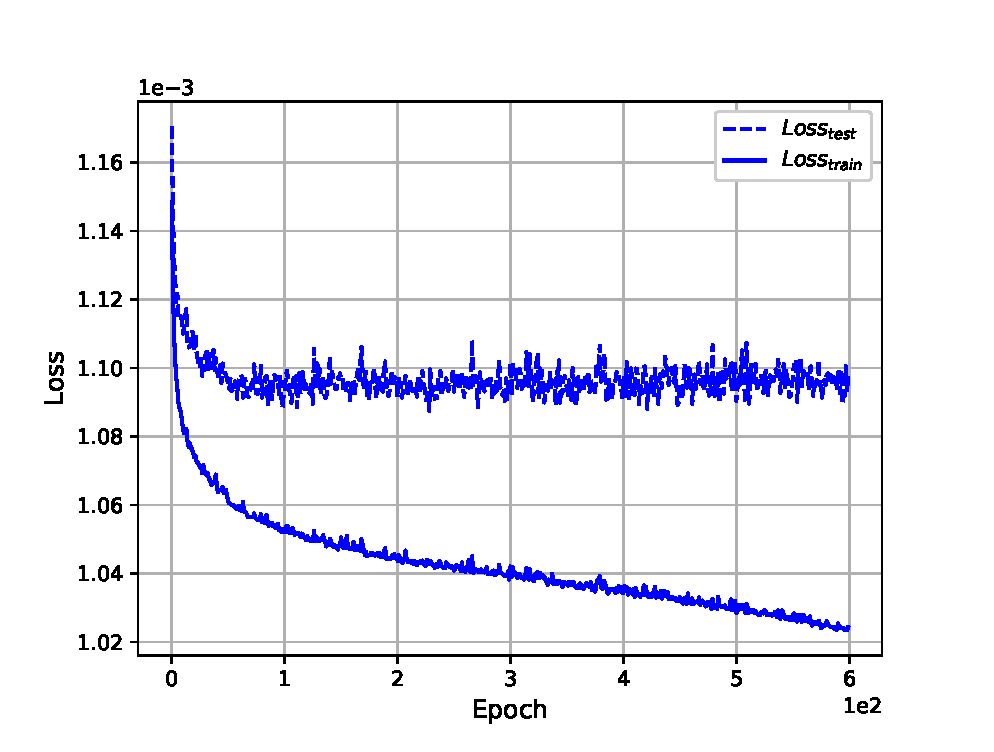
\includegraphics[width=\textwidth]{largelr_losses}
        \caption{}
        \label{fig:lr:large}
    \end{subfigure}
    \caption[Classifier loss for different learning rates]{Loss behaviour for learning rates of different scales. Figure~\subref{fig:lr:small} shows losses for \num{0.001} and figure~\subref{fig:lr:large} for~\num{0.2}.}
	\label{fig:lr}
\end{figure}

In this setup dropout is used. That makes it a bit more difficult to see the clear signs of overtraining. For a plot that shows it see section~\ref{sec:dropout}.

Like the learning rate the momentum was scanned over a wide range of values. Again he risk of overtraining and the amount of oscillations was evaluated against the overall training efficiency. This resulted in a final value of \num{0.3}. In addition, the test of using Nesterov momentum did not lead to any significant effects. It was therefore not utilized.

The decay parameter was tested to see its effect on the loss behaviour. Figure~\ref{fig:decay} shows the standard loss behaviour compared to losses for a decay value of \num{1e-6}. When decay is used the losses~\ref{fig:decay:decay} become slightly more stable and plateau a bit earlier and at a greater value. Overall no significant improvement is visible. For that reason decay is not included in the final setup of the classifier. It was kept as an option for the later combination of the classifier and the adversary where it might help keeping the model close to the optimum while slowly updating to a model less sensitive to systematics.

\begin{figure}[htbp]
    \centering
    \begin{subfigure}[b]{0.45\textwidth}
        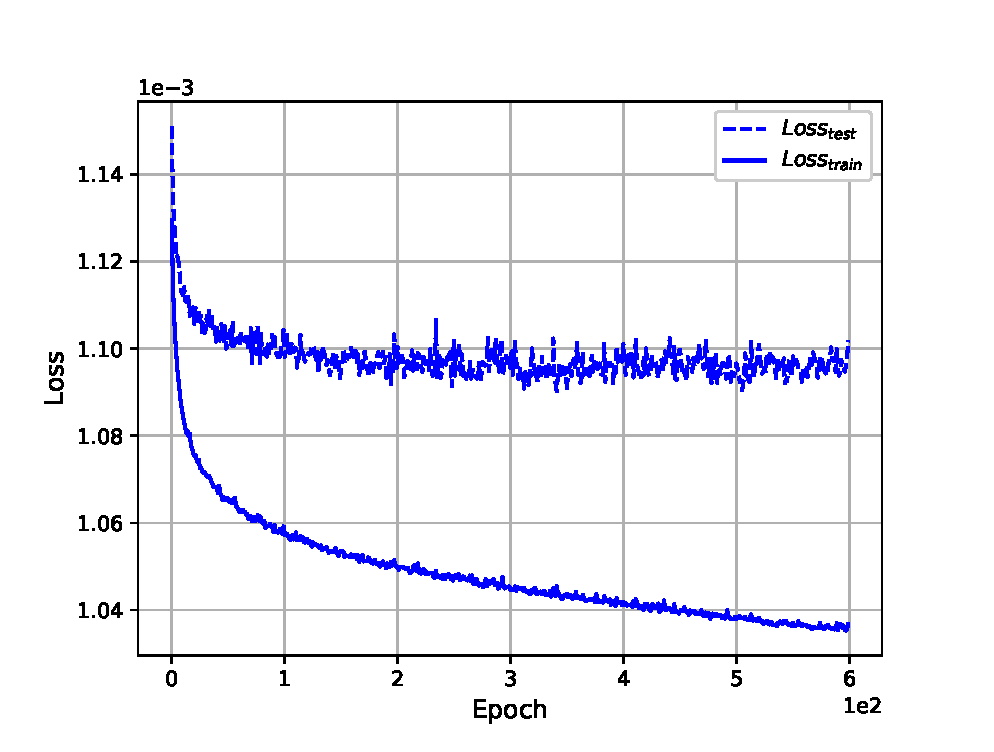
\includegraphics[width=\textwidth]{standard_losses}
        \caption{}
        \label{fig:decay:standard}
    \end{subfigure}
\quad
    \begin{subfigure}[b]{0.45\textwidth}
        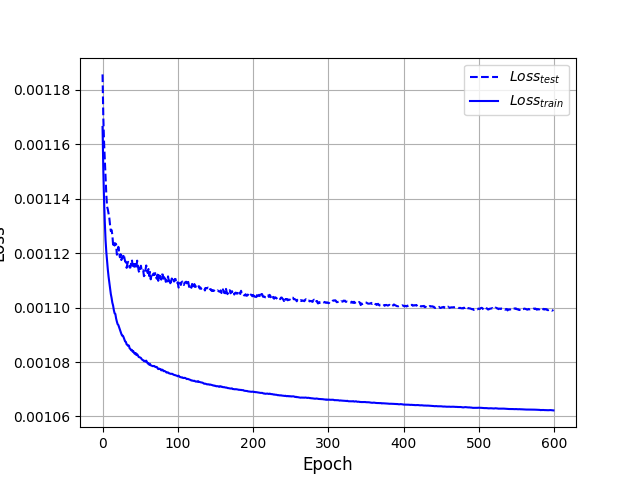
\includegraphics[width=\textwidth]{decay_losses}
        \caption{}
        \label{fig:decay:decay}
    \end{subfigure}
    \caption[Performance of the classifier with decay]{Comparison of usual loss behaviour and loss behaviour including a decay paramter. Figure~\subref{fig:decay:standard} shows the losses without decay. Figure~\subref{fig:decay:decay} shows the losses for a decay parameter of \num{1e-6}}
	\label{fig:decay}
\end{figure}




\section{Regularisation}

The two regularisation tools tested were dropout-layers and batch-normalisation layers. Dropout has the main purpose of regularising a network while batch-normalisation focuses on keeping all outputs on the same order which indirectly also helps the regularisation of the network.
Dropout is tested for a range of values defining the percentage of nodes turned off per iteration step. Batch-normalisation is just tested in the default setup to investigate its effects.

\subsection{Dropout}
\label{sec:dropout}

A dropout layer is added to each hidden layer of the network.
Figure~\ref{fig:dropout} shows the impact of dropout on the behaviour of the losses. For only \num{1} percent dropout, compared to the default \num{10} percent, overtraining occurs relatively early. For a very high dropout of \num{80} percent the losses behave strangely. The curve becomes more linear and converges less efficiently. In conclusion, dropout is a valuable addition to the network. It makes changing the architecture and the optimiser more pardoning and is a simple way to adjust a network without rearranging all hyper-parameters.

\begin{figure}[htbp]
    \centering
    \begin{subfigure}[b]{0.45\textwidth}
        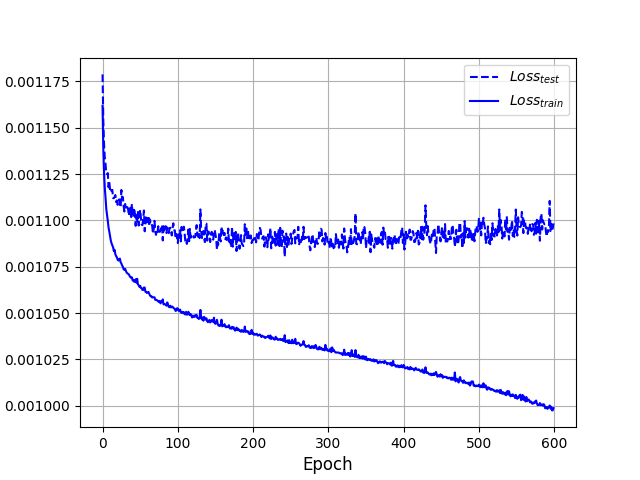
\includegraphics[width=\textwidth]{lowdrop_losses}
        \caption{}
        \label{fig:dropout:low}
    \end{subfigure}
\quad
    \begin{subfigure}[b]{0.45\textwidth}
        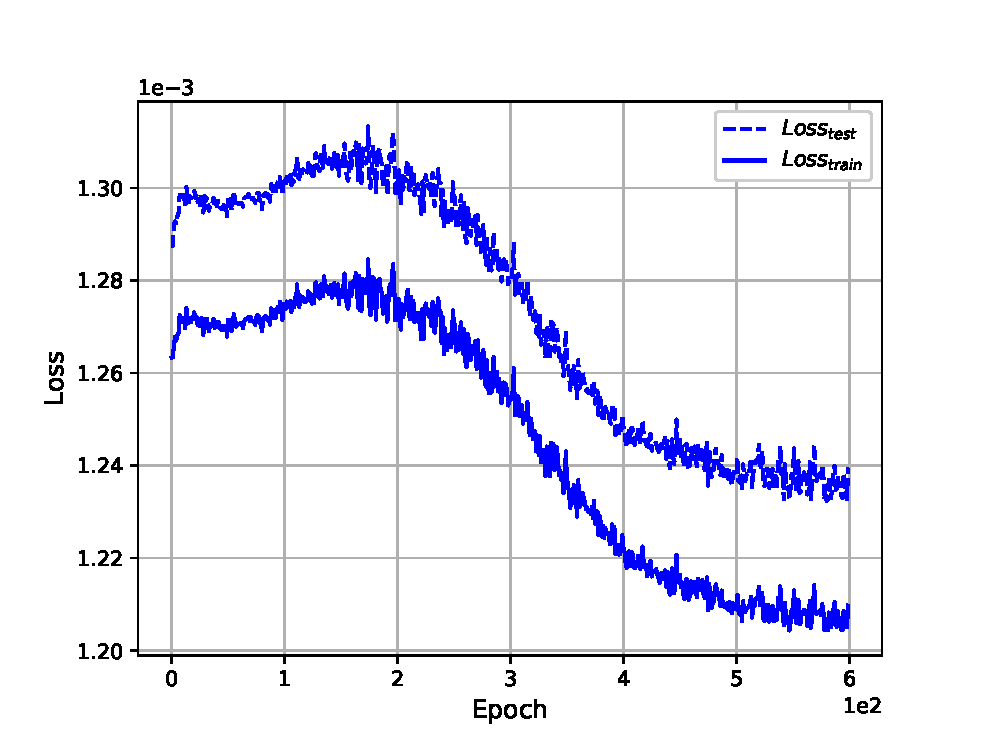
\includegraphics[width=\textwidth]{highdrop_losses}
        \caption{}
        \label{fig:dropout:high}
    \end{subfigure}
    \caption[Performance of the classifier for different dropout percentages]{Comparison of usual loss behaviour and loss behaviour including high dropout. Figure~\subref{fig:dropout:low} shows the losses for a dropout of \num{0.01}. Figure~\subref{fig:dropout:high} shows the losses for a dropout of \num{0.8}}
	\label{fig:dropout}
\end{figure}


\subsection{Batch normalisation}

Batch normalisation was added to every deep layer and it had no significant effects of the output. Either the model does not develop any overly dominant features or dropout already does a sufficient job of normalisation. Anyway, the extra layers were discarded for the classifying network to not further increase the computational time needed.

\todo{appendix}
% GNUPLOT: LaTeX picture with Postscript
\begingroup
  \makeatletter
  \providecommand\color[2][]{%
    \GenericError{(gnuplot) \space\space\space\@spaces}{%
      Package color not loaded in conjunction with
      terminal option `colourtext'%
    }{See the gnuplot documentation for explanation.%
    }{Either use 'blacktext' in gnuplot or load the package
      color.sty in LaTeX.}%
    \renewcommand\color[2][]{}%
  }%
  \providecommand\includegraphics[2][]{%
    \GenericError{(gnuplot) \space\space\space\@spaces}{%
      Package graphicx or graphics not loaded%
    }{See the gnuplot documentation for explanation.%
    }{The gnuplot epslatex terminal needs graphicx.sty or graphics.sty.}%
    \renewcommand\includegraphics[2][]{}%
  }%
  \providecommand\rotatebox[2]{#2}%
  \@ifundefined{ifGPcolor}{%
    \newif\ifGPcolor
    \GPcolortrue
  }{}%
  \@ifundefined{ifGPblacktext}{%
    \newif\ifGPblacktext
    \GPblacktexttrue
  }{}%
  % define a \g@addto@macro without @ in the name:
  \let\gplgaddtomacro\g@addto@macro
  % define empty templates for all commands taking text:
  \gdef\gplbacktext{}%
  \gdef\gplfronttext{}%
  \makeatother
  \ifGPblacktext
    % no textcolor at all
    \def\colorrgb#1{}%
    \def\colorgray#1{}%
  \else
    % gray or color?
    \ifGPcolor
      \def\colorrgb#1{\color[rgb]{#1}}%
      \def\colorgray#1{\color[gray]{#1}}%
      \expandafter\def\csname LTw\endcsname{\color{white}}%
      \expandafter\def\csname LTb\endcsname{\color{black}}%
      \expandafter\def\csname LTa\endcsname{\color{black}}%
      \expandafter\def\csname LT0\endcsname{\color[rgb]{1,0,0}}%
      \expandafter\def\csname LT1\endcsname{\color[rgb]{0,1,0}}%
      \expandafter\def\csname LT2\endcsname{\color[rgb]{0,0,1}}%
      \expandafter\def\csname LT3\endcsname{\color[rgb]{1,0,1}}%
      \expandafter\def\csname LT4\endcsname{\color[rgb]{0,1,1}}%
      \expandafter\def\csname LT5\endcsname{\color[rgb]{1,1,0}}%
      \expandafter\def\csname LT6\endcsname{\color[rgb]{0,0,0}}%
      \expandafter\def\csname LT7\endcsname{\color[rgb]{1,0.3,0}}%
      \expandafter\def\csname LT8\endcsname{\color[rgb]{0.5,0.5,0.5}}%
    \else
      % gray
      \def\colorrgb#1{\color{black}}%
      \def\colorgray#1{\color[gray]{#1}}%
      \expandafter\def\csname LTw\endcsname{\color{white}}%
      \expandafter\def\csname LTb\endcsname{\color{black}}%
      \expandafter\def\csname LTa\endcsname{\color{black}}%
      \expandafter\def\csname LT0\endcsname{\color{black}}%
      \expandafter\def\csname LT1\endcsname{\color{black}}%
      \expandafter\def\csname LT2\endcsname{\color{black}}%
      \expandafter\def\csname LT3\endcsname{\color{black}}%
      \expandafter\def\csname LT4\endcsname{\color{black}}%
      \expandafter\def\csname LT5\endcsname{\color{black}}%
      \expandafter\def\csname LT6\endcsname{\color{black}}%
      \expandafter\def\csname LT7\endcsname{\color{black}}%
      \expandafter\def\csname LT8\endcsname{\color{black}}%
    \fi
  \fi
    \setlength{\unitlength}{0.0500bp}%
    \ifx\gptboxheight\undefined%
      \newlength{\gptboxheight}%
      \newlength{\gptboxwidth}%
      \newsavebox{\gptboxtext}%
    \fi%
    \setlength{\fboxrule}{0.5pt}%
    \setlength{\fboxsep}{1pt}%
\begin{picture}(7200.00,5040.00)%
    \gplgaddtomacro\gplbacktext{%
      \csname LTb\endcsname%
      \put(594,440){\makebox(0,0)[r]{\strut{}$0$}}%
      \csname LTb\endcsname%
      \put(594,1228){\makebox(0,0)[r]{\strut{}$0.2$}}%
      \csname LTb\endcsname%
      \put(594,2016){\makebox(0,0)[r]{\strut{}$0.4$}}%
      \csname LTb\endcsname%
      \put(594,2805){\makebox(0,0)[r]{\strut{}$0.6$}}%
      \csname LTb\endcsname%
      \put(594,3593){\makebox(0,0)[r]{\strut{}$0.8$}}%
      \csname LTb\endcsname%
      \put(594,4381){\makebox(0,0)[r]{\strut{}$1$}}%
      \csname LTb\endcsname%
      \put(1334,220){\makebox(0,0){\strut{}$-4$}}%
      \csname LTb\endcsname%
      \put(2549,220){\makebox(0,0){\strut{}$-2$}}%
      \csname LTb\endcsname%
      \put(3765,220){\makebox(0,0){\strut{}$0$}}%
      \csname LTb\endcsname%
      \put(4980,220){\makebox(0,0){\strut{}$2$}}%
      \csname LTb\endcsname%
      \put(6195,220){\makebox(0,0){\strut{}$4$}}%
    }%
    \gplgaddtomacro\gplfronttext{%
      \csname LTb\endcsname%
      \put(5816,4602){\makebox(0,0)[r]{\strut{}$\frac{1}{1+e^{-x}}$}}%
    }%
    \gplbacktext
    \put(0,0){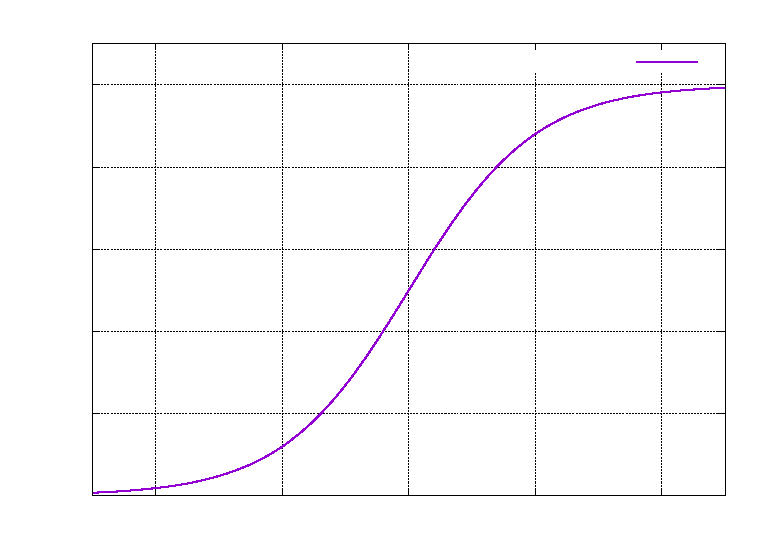
\includegraphics{sigmoid}}%
    \gplfronttext
  \end{picture}%
\endgroup

\chapter{Adversarial Neural Network}
\section{Setup of the first network}
\section{Setup of the second network}

\chapter{Conclusions}

The work presented in this thesis focussed on two issues of neural networks. The first one concerns the behaviour of neural networks and adversarial neural networks for classification tasks in particle physics. Here, the influence of the hyper-parameters on network performance for different setups was tested in order to understand how a classifier should be set up and how it can be upgraded to an adversarial neural network.

The second one addresses the possibilities offered by adversarial neural networks to limit the influence of systematic uncertainties on a classification model. In particular, the technique of an adversarial network was tested on the \tW-\ttbar separation and the systematic uncertainty arising from the different simulation approaches of DR and DS for the interference term at NLO.

A fundamental knowledge of neural networks and a set of hyper-parameters were discussed. It was shown that a good set of parameters is not only dependent on the topology of the problem but also massively depends on the setup of the network structure. A good classifier does not generally also form a good basis for an adversarial network structure. Instead, an adversarial network requires a low learning rate and above all a slow optimisation because more features of the problem need to be taken into account. This is due to the sensitivity to a certain systematic being added to the primary task of classification. The initial optimum, established for the classifier alone, that allowed for straightforward and fast training is not the desired model anymore.

Moreover, the adversarial neural network tested in this work is relatively unstable and the outcome changes significantly when hyper-parameters are slightly adjusted. This effect was not observed for the classifying network and resulted in a laborious optimisation process, which made the constraint of computational power even more significant.
The most important feature of the adversarial network, investigated with the three approaches presented in chapter~\ref{chp:ANN}, is the dimension of input it is provided with. There is a strong argument that only a single node, as classically suggested, does not justify a complex adversarial network architecture. In addition to that, the general information lost when looking only at the final node should not be neglected during the setup. The performances achieved were strongly dependent on the shape of input.

Lastly, a significant improvement on the sensitivity of the classifier for the systematic sample could not be achieved. Although the classifier was able to generate a model that rendered its adversary unable to learn, no significant differences were visible in the distribution. The shapes changed but, at the stage of this work, no sophisticated argument can be made for an improvement. In conclusion, switching from the single-node-input to a more complex input for the adversary seems to be the more promising approach. Combined with a different set of variables and a detailed hyper-parameter scan one might be able to achieve a reduction of sensitivity while keeping the quality of the overall classification constant.
For similar problems it would be interesting to test out the consequences of only providing the data actually affected by the systematic uncertainties to the adversary. In this work the systematics only affected the \tW-channel and the \ttbar was still considered nominal. This could have a strong bias effect on the result.

Neural networks in general are a promising technique for researchers in particle physics. The variety of highly different structures and hyper-parameters of the networks make them a potentially powerful tool for different scopes of research. An improvement in the sensitivity to systematics has been achieved for different researches using adversarial network approaches. Although a small effect on the sensitivity was achieved in this work, the sensitivity was not reduced as far as hoped for. Perhaps the topology of the problem and the shape of the systematics mean that the task has no model that is insensitive. However, the strategies presented in this work, pave the way for further research focusing on the approach and the appliance of machine learning techniques for data analysis in particle physics.


% Uncomment the following command to get references per chapter.
% Put it inside the file or change \include to \input if you do not want the references
% on a separate page
% \printbibliography[heading=subbibliography]

%------------------------------------------------------------------------------
% Use biblatex for the bibliography
% Add bibliography to Table of Contents
% Comment out this command if your references are printed for each chapter.
\printbibliography[heading=bibintoc]

%------------------------------------------------------------------------------
% Include the following lines and comment out \printbibliography if
% you use BiBTeX for the bibliography.
% If you use biblatex package the files should be specified in the preamble.
% \KOMAoptions{toc=bibliography}
% {\raggedright
%   \bibliographystyle{../refs/atlasBibStyleWithTitle.bst}
%   % \bibliographystyle{unsrt}
%   \bibliography{./thesis_refs,../refs/standard_refs-bibtex}
% }

%------------------------------------------------------------------------------
\appendix
% \part*{Appendix}
% Add your appendices here - don't forget to also add them to \includeonly above
%------------------------------------------------------------------------------
\chapter{Monte Carlo simulations}
\label{sec:app}
%------------------------------------------------------------------------------
The following section provides the technical details for the Monte Carlo simulations used in this work.
All of the sets are distributed by the SingleTop group at ATLAS. The sets used are v23 sets from Release 21.
They were filtered to only the \texttt{2j2b} region.

\begin{table}[h]
\begin{tabular}{llll}
DSID & $\sigma [pb]$ & $k$-factor & Tags\\
Single top-quark, \tW-channel, DR&  &  &  \\ \hline
410648& \num{4.0} & \num{0.94}  & e6615\_e5984\_s3126\_r9364\_r9315\_p3409\\
410649& \num{3.99} & \num{0.95} & e6615\_e5984\_a875\_r9364\_r9315\_p3526\\ \hline
Single top-quark, \tW-channel, DS&  &  &  \\ \hline
410656& \num{3.89} & \num{0.97} & e6615\_e5984\_s3126\_r10201\_r10210\_p3409\\
410657& \num{3.97} & \num{0.95} & e6615\_e5984\_s3126\_r10201\_r10210\_p3409\\ \hline
Top-quark pair&  &  &  \\ \hline
410657& \num{76.95} & \num{1.14} & e6348\_e5984\_a875\_r10201\_r10210\_p3554
\end{tabular}
\caption[DSID list]{MC samples used in this thesis.}
\label{tab:DSID}
\end{table}

%%% Local Variables: 
%%% mode: latex
%%% TeX-master: "../mythesis"
%%% End: 

% \printbibliography[heading=subbibliography]

%------------------------------------------------------------------------------
% Declare lists of figures and tables and acknowledgements as backmatter
% Chapter/section numbers are turned off
\backmatter

\listoffigures
\listoftables

%------------------------------------------------------------------------------
% Print the glossary and list of acronyms
% \printglossaries

%------------------------------------------------------------------------------
% You could instead add your acknowledgements here - don't forget to
% also add them to \includeonly above
% %------------------------------------------------------------------------------
\chapter*{Danksagung}
\label{sec:ack}
%------------------------------------------------------------------------------

Ich möchte mich bei meinem Vater bedanken, dass er seine Faszination für die Wissenschaft mit mir geteilt hat.
Ich bedanke mich bei Ian {C.} Brock für die Möglichkeit, diese Arbeit zu verfassen, für seine Ermutigung zu neuen Projekten und für die Fähigkeit, seiner Arbeitsgruppe ein Gefühl von Zusammenhalt zu geben

Meiner Familie und meinen Freunden danke ich, dass sie die Stütze für mich waren, ohne die ich diese Arbeit nie hätten schreiben können.
Für all die Hilfe, für ermutigende Worte, für die Brettspiel-Abende und Kaffeepausen und nicht zuletzt für all die angeregten Diskussionen kann ich allen anderen Mitgliedern der Arbeitsgruppe nicht genug danken.


%%% Local Variables: 
%%% mode: latex
%%% TeX-master: "../mythesis"
%%% End: 


%------------------------------------------------------------------------------
% CV needed when you submit your PhD thesis
% \definecolor{lightgray}{gray}{0.8}
\newcolumntype{L}{>{\raggedleft}p{0.15\textwidth}}
\newcolumntype{R}{p{0.8\textwidth}}
\newcommand\VRule{\color{lightgray}\vrule width 0.5pt}

\thispagestyle{empty}
\section*{Curriculum Vitae}

\subsection*{Personal Details}

\begin{tabular}{L!{\VRule}R}
Name & Johann Schmidt \\
Date of Birth &  \\
Email & abc@physik.uni-def.de \\
Family status & Single
\end{tabular}

\subsection*{Education}

\begin{tabular}{L!{\VRule}R}
1997--2003 & Abitur, ABC Secondary School, Hamburg, Germany\\
2004--2007 & BSc in Physics, Rheinische Friedrich-Wilhelms-Universität, Bonn, Germany.\\
2006 & CERN Summer Student, Geneva, Switzerland. \\
2007--2009 &  MSc in Physics Rheinische Friedrich-Wilhelms-Universität, Bonn, Germany. \\
2009--2012 &  PhD in Physics, Rheinische Friedrich-Wilhelms-Universität, Bonn, Germany. \\
2012 & Advanced Data Analysis School, Frankfurt, Germany.
\end{tabular}

\subsection*{Professional Experience}

\begin{tabular}{L!{\VRule}R}
2004 & Summer Student at CERN, Geneva, Switzerland. \\
2007--2012 & Doctoral work at the University of Bonn, Germany. \\
2008--2009 & Fieldwork at CERN, Geneva, Switzerland.\\
2011 & Talk at the Advanced Physics Conference, Timbucto
\end{tabular}

\subsection*{Languages}
\begin{tabular}{L!{\VRule}R}
German & Mother tongue \\
English & Fluent \\
Russian & Basic
\end{tabular}


\end{document}

%%% Local Variables:
%%% mode: latex
%%% TeX-master: t
%%% End:
